% $Author$
% $Date$
% $Revision$
% $Id$

% HISTORY:
% 2007-10-29 - Oscar started chapter
% 2007-11-30 - Oscar first draft
% 2007-12-07 - Orla Greevy reviewed
% 2007-12-09 - Lukas Renggli reviewed
% 2008-01-11 - Andrew revised
% 2009-04-17 - Fabrizio Perin reviewed
% 2009-04-18 - Jorge Ressia reviewed
% 2009-05-06 - Oscar converted to Pharo; fixed review comments

%=================================================================
\ifx\wholebook\relax\else
% --------------------------------------------
% Lulu:
	\documentclass[a4paper,10pt,twoside]{book}
	\usepackage[
		papersize={6.13in,9.21in},
		hmargin={.75in,.75in},
		vmargin={.75in,1in},
		ignoreheadfoot
	]{geometry}
	% $Author$
% $Date$
% $Revision$

% HISTORY:
% 2006-10-31 - Oscar code macros
% ...

%=============================================================
% NB: documentclass must be set in main document.
% Allows book to be generated in multiple formats.
%=============================================================
%:Packages
\usepackage[T1]{fontenc}  %%%%%% really important to get the code directly in the text!
\usepackage{lmodern}
%\usepackage[scaled=0.85]{bookmanx} % needs another scale factor if used with \renewcommand{\sfdefault}{cmbr}
\usepackage{palatino}
\usepackage[scaled=0.85]{helvet}
\usepackage[protrusion,expansion=false]{microtype}
\usepackage{graphicx}
\usepackage{theorem}
\usepackage[english]{babel}
%%% ON: pdfsync breaks the use of p{width} for tabular columns!
%%\ifdefined\usepdfsync\usepackage{pdfsync}\fi % Requires texlive 2007
%=============================================================
%:More packages
%Stef should check which ones are used!
%\usepackage{picinpar}
%\usepackage{layout}
%\usepackage{color}
%\usepackage{enum}
%\usepackage{a4wide}
% \usepackage{fancyhdr}
\usepackage{ifthen}
\usepackage{float}
\usepackage{longtable}
\usepackage{makeidx}
\usepackage[nottoc]{tocbibind}
\usepackage{multicol}
\usepackage{booktabs}	% book-style tables
\usepackage{topcapt}	% enables \topcaption
\usepackage{multirow}
\usepackage{tabularx}
%\usepackage[bottom]{footmisc}
\usepackage{xspace}
\usepackage{alltt}
\usepackage{amssymb,textcomp}
\usepackage[usenames,dvipsnames]{color}
%\usepackage{colortbl}
\usepackage[hang]{subfigure}\makeatletter\def\p@subfigure{\thefigure\,}\makeatother
\usepackage{rotating}
\usepackage{enumitem}	% apb: allows more control over tags in enumerations
\usepackage{verbatim}     % for comment environment
\usepackage{varioref}	% for page references that work
\labelformat{footnote}{\thechapter--#1} % to distinguish citations from jurabib
\usepackage{needspace}
\usepackage{isodateo} % enable \isodate
\usepackage[newparttoc]{titlesec}
\usepackage{titletoc}
\usepackage{wrapfig}
\usepackage[
	super,
	citefull=first,
	authorformat={allreversed,and},
	titleformat={commasep,italic}
]{jurabib} % citations as footnotes
\usepackage[
	colorlinks=true,
	linkcolor=black,
	urlcolor=black,
	citecolor=black
]{hyperref}   % should come last
%=============================================================
%:PDF version
%%\pdfminorversion=3 % Set PDF to 1.3 for Lulu
%=============================================================
%:URL style
\makeatletter
\def\url@leostyle{%
  \@ifundefined{selectfont}{\def\UrlFont{\sf}}{\def\UrlFont{\sffamily}}}
\makeatother
% Now actually use the newly defined style.
\urlstyle{leo}
%=============================================================
%:Booleans
\newboolean{lulu}
\setboolean{lulu}{false}
\newcommand{\ifluluelse}[2]{\ifthenelse{\boolean{lulu}}{#1}{#2}}
%=============================================================
%:Names
\newcommand{\SUnit}{SUnit\xspace}
\newcommand{\sunit}{SUnit\xspace}
\newcommand{\xUnit}{$x$Unit\xspace}
\newcommand{\JUnit}{JUnit\xspace}
\newcommand{\st}{Smalltalk\xspace}
\newcommand{\pharo}{Pharo\xspace} % Use this, not \Pharo
%\newcommand{\sqmap}{SqueakMap\xspace}
\newcommand{\squeak}{Squeak\xspace} % use this, not \Squeak or \sq
\newcommand{\sqsrc}{SqueakSource\xspace}
\newcommand{\sbe}{\url{http://SqueakByExample.org}\xspace}
\newcommand{\pharoweb}{\url{http://pharo-project.org}\xspace}
\newcommand{\pbe}{\url{http://PharoByExample.org}\xspace}
\newcommand{\sba}{\url{http://SquareBracketAssociates.org}\xspace}
\newcommand{\bam}{\lct{Bounc\-ing\-Atoms\-Morph}\xspace}
%=============================================================
%:Markup macros for proof-reading
\usepackage[normalem]{ulem} % for \sout
\usepackage{xcolor}
\newcommand{\ra}{$\rightarrow$}
\newcommand{\ugh}[1]{\textcolor{red}{\uwave{#1}}} % please rephrase
\newcommand{\ins}[1]{\textcolor{blue}{\uline{#1}}} % please insert
\newcommand{\del}[1]{\textcolor{red}{\sout{#1}}} % please delete
\newcommand{\chg}[2]{\textcolor{red}{\sout{#1}}{\ra}\textcolor{blue}{\uline{#2}}} % please change
%=============================================================
%:Editorial comment macros
%\newcommand{\nnbb}[2]{
%    % \fbox{\bfseries\sffamily\scriptsize#1}
%    \fcolorbox{gray}{yellow}{\bfseries\sffamily\scriptsize#1}
%    {\sf\small$\blacktriangleright$\textit{#2}$\blacktriangleleft$}
%   }
\newcommand{\yellowbox}[1]{\fcolorbox{gray}{yellow}{\bfseries\sffamily\scriptsize#1}}
\newcommand{\triangles}[1]{{\sf\small$\blacktriangleright$\textit{#1}$\blacktriangleleft$}}
\newcommand{\nnbb}[2]{\yellowbox{#1} \triangles{#2}}
\newcommand{\fix}{\yellowbox{FIX!}}
\newcommand{\here}{\yellowbox{CONTINUE HERE!}}
% editor macros
\newcommand{\apl}[1]{\nnbb{Alain}{#1}} % Alain
\newcommand{\ab}[1]{\nnbb{Andrew}{#1}} % Black
\newcommand{\sd}[1]{\nnbb{St\'{e}f}{#1}} % Ducasse
\newcommand{\dc}[1]{\nnbb{DamienC}{#1}} % Ducasse
\newcommand{\md}[1]{\nnbb{Marcus}{#1}} % Denker
\newcommand{\on}[1]{\nnbb{Oscar}{#1}} % Nierstrasz
\newcommand{\damien}[1]{\nnbb{Damien}{#1}} % Pollet
\newcommand{\lr}[1]{\nnbb{Lukas}{#1}} % Renggli
\newcommand{\orla}[1]{\nnbb{Orla}{#1}} % Greevy
\newcommand{\alex}[1]{\nnbb{Alex}{#1}} % Bergel
\newcommand{\alx}[1]{\nnbb{Alex}{#1}} % Bergel
\newcommand{\dr}[1]{\nnbb{David}{#1}} % Roethlisberger
\newcommand{\ja}[1]{\nnbb{Jannik}{#1}} % Laval
\newcommand{\jr}[1]{\nnbb{Jorge}{#1}} % Ressia
\newcommand{\fp}[1]{\nnbb{Fabrizio}{#1}} % Perin
\newcommand{\michael}[1]{\nnbb{Michael}{#1}} % Davies
\newcommand{\ew}[1]{\nnbb{Erwann}{#1}} % Wernli
\newcommand{\mb}[1]{\nnbb{Martial}{#1}} % Boniou
\newcommand{\hw}[1]{\nnbb{Hernan}{#1}} % Wilkinson
%=============================================================
%:Abbreviation macros
\newcommand{\ie}{\emph{すなわち}、}
\newcommand{\eg}{\emph{例えば}、}
\newcommand{\etc}{などなど。}
%=============================================================
%:Cross reference macros
\newcommand{\charef}[1]{第~\ref{cha:#1}~章}
\newcommand{\secref}[1]{\ref{sec:#1}~節}
\newcommand{\figref}[1]{図~\ref{fig:#1}\xspace}
\newcommand{\Figref}[1]{図~\ref{fig:#1}\xspace}
\newcommand{\appref}[1]{付録~\ref{app:#1}\xspace}
\newcommand{\tabref}[1]{表~\ref{tab:#1}\xspace}
\newcommand{\faqref}[1]{FAQ~\ref{faq:#1}, p.~\pageref{faq:#1}\xspace}
% APB: I removed trailing \xspace commands from these macros because
% \xspace mostly doesn't work.  If you want a space after your
% references, type one!
% ON: xspace has always worked just fine for me!  Please leave them in.
%
\newcommand{\ruleref}[1]{\ref{rule:#1}\xspace}
%
\newcommand{\egref}[1]{example~\ref{eg:#1}\xspace}
\newcommand{\Egref}[1]{Example~\ref{eg:#1}\xspace}
%
\newcommand{\scrref}[1]{script~\ref{scr:#1}\xspace}
\newcommand{\Scrref}[1]{Script~\ref{scr:#1}\xspace}
\newcommand{\tscrref}[1]{the script~\ref{scr:#1}\xspace}
\newcommand{\Tscrref}[1]{The script~\ref{scr:#1}\xspace}
%
\newcommand{\mthref}[1]{method~\ref{mth:#1}\xspace}
\newcommand{\mthsref}[1]{methods~\ref{mth:#1}\xspace}
\newcommand{\Mthref}[1]{Method~\ref{mth:#1}\xspace}
\newcommand{\tmthref}[1]{the method~\ref{mth:#1}\xspace}
\newcommand{\Tmthref}[1]{The method~\ref{mth:#1}\xspace}
%
\newcommand{\clsref}[1]{class~\ref{cls:#1}\xspace}
\newcommand{\tclsref}[1]{the class~\ref{cls:#1}\xspace}
\newcommand{\Tclsref}[1]{The class~\ref{cls:#1}\xspace}

\newcommand{\chalabel}[1]{\label{cha:#1}}
\newcommand{\seclabel}[1]{\label{sec:#1}}
\newcommand{\figlabel}[1]{\label{fig:#1}}
\newcommand{\tablabel}[1]{\label{tab:#1}}
\newcommand{\rulelabel}[1]{\label{rule:#1}}
\newcommand{\eglabel}[1]{\label{eg:#1}}
\newcommand{\scrlabel}[1]{\label{scr:#1}}
\newcommand{\mthlabel}[1]{\label{mth:#1}}
\newcommand{\clslabel}[1]{\label{cls:#1}}
\newcommand{\faqlabel}[1]{\label{faq:#1}}
%=============================================================
%:Menu item macro
% for menu items, so we can change our minds on how to print them! (apb)
\definecolor{lightgray}{gray}{0.89}
\newcommand{\menu}[1]{{%
	\setlength{\fboxsep}{0pt}%
	\colorbox{lightgray}{{{\upshape\sffamily\strut \,#1\,}}}}}
\newcommand{\link}[1]{{%
	\fontfamily{lmr}\selectfont
 	\upshape{\sffamily \underline{#1}}}}
% For submenu items:
\newcommand{\go}{\,$\triangleright$\,}
% \newcommand{\go}{\,$\blacktriangleright$\,}
% For keyboard shortcuts:
%\newcommand{\short}[1]{\mbox{$\langle${\sc CMD}$\rangle$-#1}\xspace}
\newcommand{\short}[1]{\mbox{{\sc cmd}\hspace{0.08em}--\hspace{0.09em}#1}\xspace}
% For buttons:
\newcommand{\button}[1]{{%
	\setlength{\fboxsep}{0pt}%
	\fbox{{\upshape\sffamily\strut \,#1\,}}}}
% NB: The button macro does not work within captions -- incompatible with xcolor package :-(
\newcommand{\toolsflap}{\textit{Tools} flap\xspace}
%=============================================================
%:Mouse clicks
\newcommand{\click}{click\xspace} % RED
\newcommand{\actclick}{action-click\xspace} % YELLOW
\newcommand{\metaclick}{meta-click\xspace} % BLUE
\newcommand{\Click}{Click\xspace} % RED
\newcommand{\Actclick}{Action-click\xspace} % YELLOW
\newcommand{\Metaclick}{Meta-click\xspace} % BLUE
%=============================================================
%:ToSh macros
\newboolean{tosh}
\setboolean{tosh}{false}
\newcommand{\iftoshelse}[2]{\ifthenelse{\boolean{tosh}}{#1}{#2}}
%=============================================================
%:ToSh colors
%\newcommand{\highlightcolor}{\color{blue!65}}
%\newcommand{\boxcolor}{\color{gray!25}}
\newcommand{\highlight}[1]{\textcolor{blue!65}{#1}}
%\newcommand{\codecolor}{\color{blue!65}}
%%\setlength{\fboxrule}{2pt}
%\newcommand{\asPict}[1]{%
%	{\Large\highlight{#1}}}
%=============================================================
%:Reader cues (do this)
%
% Indicate something the reader should try out.
% \newcommand{\dothisicon}{\raisebox{-.5ex}{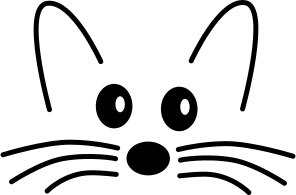
\includegraphics[width=1.4em]{squeak-logo}}}
\iftoshelse{
	\usepackage{marginnote}
		\renewcommand*{\marginfont}{\footnotesize}
	\newcommand{\vartriangleout}{\ifthenelse{\isodd{\thepage}}{\vartriangleright}{\vartriangleleft}}
	\newcommand{\dothisicon}{\fcolorbox{blue!65}{white}{\highlight{$\vartriangleout$}}}
	\newcommand{\dothis}[1]{%
		\noindent\par\noindent
		{\reversemarginpar
			\marginnote{\fcolorbox{blue!65}{white}{\highlight{$\vartriangleout$}}}}
		%\MarginLabel{do this}
		\noindent\emph{#1}
		\nopagebreak}
}{
	\newcommand{\dothisicon}{\raisebox{-.5ex}{
\includegraphics[height=1.2em]{pharo}}}
	\newcommand{\dothis}[1]{%
		\medskip
		\noindent\dothisicon
		\ifx#1\empty\else\quad\emph{#1}\fi
		\par\smallskip\nopagebreak}
}
%===> NEW VERSION <===
% NB: To use this in an individual chapter, you must set:
%\graphicspath{{figures/} {../figures/}}
% at the head of the chapter.  Don't forget the final /
%=============================================================
%:Reader hints (hint)
%
% Indicates a non-obvious consequence 
\newcommand{\hint}[1]{\vspace{1ex}\noindent\fbox{\textsc{Hint}} \emph{#1}}
%=================================================================
% graphics for Morphic handles
\newcommand{\grabHandle}{\raisebox{-0.2ex}{
\includegraphics[width=1em]{blackHandle}}}
\newcommand{\moveHandle}{\raisebox{-0.2ex}{
\includegraphics[width=1em]{moveHandle}}}
\newcommand{\debugHandle}{\raisebox{-0.2ex}{
\includegraphics[width=1em]{debugHandle}}}
%=============================================================
%:Highlighting Important stuff (doublebox)
%
% From Seaside book ...
\newsavebox{\SavedText}
\newlength{\InnerBoxRule}\setlength{\InnerBoxRule}{.75\fboxrule}
\newlength{\OuterBoxRule}\setlength{\OuterBoxRule}{1.5\fboxrule}
\newlength{\BoxSeparation}\setlength{\BoxSeparation}{1.5\fboxrule}
\addtolength{\BoxSeparation}{.5pt}
\newlength{\SaveBoxSep}\setlength{\SaveBoxSep}{2\fboxsep}
%
\newenvironment{doublebox}{\begin{lrbox}{\SavedText}
    \begin{minipage}{.75\textwidth}}
    {\end{minipage}\end{lrbox}\begin{center}
    \setlength{\fboxsep}{\BoxSeparation}\setlength{\fboxrule}{\OuterBoxRule}
    \fbox{\setlength{\fboxsep}{\SaveBoxSep}\setlength{\fboxrule}{\InnerBoxRule}%
      \fbox{\usebox{\SavedText}}}
  \end{center}}
% Use this:
\newcommand{\important}[1]{\begin{doublebox}#1\end{doublebox}}
%=============================================================
%:Section depth
\setcounter{secnumdepth}{2}
%% for this to happen start the file with
%\ifx\wholebook\relax\else
%% $Author$
% $Date$
% $Revision$

% HISTORY:
% 2006-10-31 - Oscar code macros
% ...

%=============================================================
% NB: documentclass must be set in main document.
% Allows book to be generated in multiple formats.
%=============================================================
%:Packages
\usepackage[T1]{fontenc}  %%%%%% really important to get the code directly in the text!
\usepackage{lmodern}
%\usepackage[scaled=0.85]{bookmanx} % needs another scale factor if used with \renewcommand{\sfdefault}{cmbr}
\usepackage{palatino}
\usepackage[scaled=0.85]{helvet}
\usepackage[protrusion,expansion=false]{microtype}
\usepackage{graphicx}
\usepackage{theorem}
\usepackage[english]{babel}
%%% ON: pdfsync breaks the use of p{width} for tabular columns!
%%\ifdefined\usepdfsync\usepackage{pdfsync}\fi % Requires texlive 2007
%=============================================================
%:More packages
%Stef should check which ones are used!
%\usepackage{picinpar}
%\usepackage{layout}
%\usepackage{color}
%\usepackage{enum}
%\usepackage{a4wide}
% \usepackage{fancyhdr}
\usepackage{ifthen}
\usepackage{float}
\usepackage{longtable}
\usepackage{makeidx}
\usepackage[nottoc]{tocbibind}
\usepackage{multicol}
\usepackage{booktabs}	% book-style tables
\usepackage{topcapt}	% enables \topcaption
\usepackage{multirow}
\usepackage{tabularx}
%\usepackage[bottom]{footmisc}
\usepackage{xspace}
\usepackage{alltt}
\usepackage{amssymb,textcomp}
\usepackage[usenames,dvipsnames]{color}
%\usepackage{colortbl}
\usepackage[hang]{subfigure}\makeatletter\def\p@subfigure{\thefigure\,}\makeatother
\usepackage{rotating}
\usepackage{enumitem}	% apb: allows more control over tags in enumerations
\usepackage{verbatim}     % for comment environment
\usepackage{varioref}	% for page references that work
\labelformat{footnote}{\thechapter--#1} % to distinguish citations from jurabib
\usepackage{needspace}
\usepackage{isodateo} % enable \isodate
\usepackage[newparttoc]{titlesec}
\usepackage{titletoc}
\usepackage{wrapfig}
\usepackage[
	super,
	citefull=first,
	authorformat={allreversed,and},
	titleformat={commasep,italic}
]{jurabib} % citations as footnotes
\usepackage[
	colorlinks=true,
	linkcolor=black,
	urlcolor=black,
	citecolor=black
]{hyperref}   % should come last
%=============================================================
%:PDF version
%%\pdfminorversion=3 % Set PDF to 1.3 for Lulu
%=============================================================
%:URL style
\makeatletter
\def\url@leostyle{%
  \@ifundefined{selectfont}{\def\UrlFont{\sf}}{\def\UrlFont{\sffamily}}}
\makeatother
% Now actually use the newly defined style.
\urlstyle{leo}
%=============================================================
%:Booleans
\newboolean{lulu}
\setboolean{lulu}{false}
\newcommand{\ifluluelse}[2]{\ifthenelse{\boolean{lulu}}{#1}{#2}}
%=============================================================
%:Names
\newcommand{\SUnit}{SUnit\xspace}
\newcommand{\sunit}{SUnit\xspace}
\newcommand{\xUnit}{$x$Unit\xspace}
\newcommand{\JUnit}{JUnit\xspace}
\newcommand{\st}{Smalltalk\xspace}
\newcommand{\pharo}{Pharo\xspace} % Use this, not \Pharo
%\newcommand{\sqmap}{SqueakMap\xspace}
\newcommand{\squeak}{Squeak\xspace} % use this, not \Squeak or \sq
\newcommand{\sqsrc}{SqueakSource\xspace}
\newcommand{\sbe}{\url{http://SqueakByExample.org}\xspace}
\newcommand{\pharoweb}{\url{http://pharo-project.org}\xspace}
\newcommand{\pbe}{\url{http://PharoByExample.org}\xspace}
\newcommand{\sba}{\url{http://SquareBracketAssociates.org}\xspace}
\newcommand{\bam}{\lct{Bounc\-ing\-Atoms\-Morph}\xspace}
%=============================================================
%:Markup macros for proof-reading
\usepackage[normalem]{ulem} % for \sout
\usepackage{xcolor}
\newcommand{\ra}{$\rightarrow$}
\newcommand{\ugh}[1]{\textcolor{red}{\uwave{#1}}} % please rephrase
\newcommand{\ins}[1]{\textcolor{blue}{\uline{#1}}} % please insert
\newcommand{\del}[1]{\textcolor{red}{\sout{#1}}} % please delete
\newcommand{\chg}[2]{\textcolor{red}{\sout{#1}}{\ra}\textcolor{blue}{\uline{#2}}} % please change
%=============================================================
%:Editorial comment macros
%\newcommand{\nnbb}[2]{
%    % \fbox{\bfseries\sffamily\scriptsize#1}
%    \fcolorbox{gray}{yellow}{\bfseries\sffamily\scriptsize#1}
%    {\sf\small$\blacktriangleright$\textit{#2}$\blacktriangleleft$}
%   }
\newcommand{\yellowbox}[1]{\fcolorbox{gray}{yellow}{\bfseries\sffamily\scriptsize#1}}
\newcommand{\triangles}[1]{{\sf\small$\blacktriangleright$\textit{#1}$\blacktriangleleft$}}
\newcommand{\nnbb}[2]{\yellowbox{#1} \triangles{#2}}
\newcommand{\fix}{\yellowbox{FIX!}}
\newcommand{\here}{\yellowbox{CONTINUE HERE!}}
% editor macros
\newcommand{\apl}[1]{\nnbb{Alain}{#1}} % Alain
\newcommand{\ab}[1]{\nnbb{Andrew}{#1}} % Black
\newcommand{\sd}[1]{\nnbb{St\'{e}f}{#1}} % Ducasse
\newcommand{\dc}[1]{\nnbb{DamienC}{#1}} % Ducasse
\newcommand{\md}[1]{\nnbb{Marcus}{#1}} % Denker
\newcommand{\on}[1]{\nnbb{Oscar}{#1}} % Nierstrasz
\newcommand{\damien}[1]{\nnbb{Damien}{#1}} % Pollet
\newcommand{\lr}[1]{\nnbb{Lukas}{#1}} % Renggli
\newcommand{\orla}[1]{\nnbb{Orla}{#1}} % Greevy
\newcommand{\alex}[1]{\nnbb{Alex}{#1}} % Bergel
\newcommand{\alx}[1]{\nnbb{Alex}{#1}} % Bergel
\newcommand{\dr}[1]{\nnbb{David}{#1}} % Roethlisberger
\newcommand{\ja}[1]{\nnbb{Jannik}{#1}} % Laval
\newcommand{\jr}[1]{\nnbb{Jorge}{#1}} % Ressia
\newcommand{\fp}[1]{\nnbb{Fabrizio}{#1}} % Perin
\newcommand{\michael}[1]{\nnbb{Michael}{#1}} % Davies
\newcommand{\ew}[1]{\nnbb{Erwann}{#1}} % Wernli
\newcommand{\mb}[1]{\nnbb{Martial}{#1}} % Boniou
\newcommand{\hw}[1]{\nnbb{Hernan}{#1}} % Wilkinson
%=============================================================
%:Abbreviation macros
\newcommand{\ie}{\emph{すなわち}、}
\newcommand{\eg}{\emph{例えば}、}
\newcommand{\etc}{などなど。}
%=============================================================
%:Cross reference macros
\newcommand{\charef}[1]{第~\ref{cha:#1}~章}
\newcommand{\secref}[1]{\ref{sec:#1}~節}
\newcommand{\figref}[1]{図~\ref{fig:#1}\xspace}
\newcommand{\Figref}[1]{図~\ref{fig:#1}\xspace}
\newcommand{\appref}[1]{付録~\ref{app:#1}\xspace}
\newcommand{\tabref}[1]{表~\ref{tab:#1}\xspace}
\newcommand{\faqref}[1]{FAQ~\ref{faq:#1}, p.~\pageref{faq:#1}\xspace}
% APB: I removed trailing \xspace commands from these macros because
% \xspace mostly doesn't work.  If you want a space after your
% references, type one!
% ON: xspace has always worked just fine for me!  Please leave them in.
%
\newcommand{\ruleref}[1]{\ref{rule:#1}\xspace}
%
\newcommand{\egref}[1]{example~\ref{eg:#1}\xspace}
\newcommand{\Egref}[1]{Example~\ref{eg:#1}\xspace}
%
\newcommand{\scrref}[1]{script~\ref{scr:#1}\xspace}
\newcommand{\Scrref}[1]{Script~\ref{scr:#1}\xspace}
\newcommand{\tscrref}[1]{the script~\ref{scr:#1}\xspace}
\newcommand{\Tscrref}[1]{The script~\ref{scr:#1}\xspace}
%
\newcommand{\mthref}[1]{method~\ref{mth:#1}\xspace}
\newcommand{\mthsref}[1]{methods~\ref{mth:#1}\xspace}
\newcommand{\Mthref}[1]{Method~\ref{mth:#1}\xspace}
\newcommand{\tmthref}[1]{the method~\ref{mth:#1}\xspace}
\newcommand{\Tmthref}[1]{The method~\ref{mth:#1}\xspace}
%
\newcommand{\clsref}[1]{class~\ref{cls:#1}\xspace}
\newcommand{\tclsref}[1]{the class~\ref{cls:#1}\xspace}
\newcommand{\Tclsref}[1]{The class~\ref{cls:#1}\xspace}

\newcommand{\chalabel}[1]{\label{cha:#1}}
\newcommand{\seclabel}[1]{\label{sec:#1}}
\newcommand{\figlabel}[1]{\label{fig:#1}}
\newcommand{\tablabel}[1]{\label{tab:#1}}
\newcommand{\rulelabel}[1]{\label{rule:#1}}
\newcommand{\eglabel}[1]{\label{eg:#1}}
\newcommand{\scrlabel}[1]{\label{scr:#1}}
\newcommand{\mthlabel}[1]{\label{mth:#1}}
\newcommand{\clslabel}[1]{\label{cls:#1}}
\newcommand{\faqlabel}[1]{\label{faq:#1}}
%=============================================================
%:Menu item macro
% for menu items, so we can change our minds on how to print them! (apb)
\definecolor{lightgray}{gray}{0.89}
\newcommand{\menu}[1]{{%
	\setlength{\fboxsep}{0pt}%
	\colorbox{lightgray}{{{\upshape\sffamily\strut \,#1\,}}}}}
\newcommand{\link}[1]{{%
	\fontfamily{lmr}\selectfont
 	\upshape{\sffamily \underline{#1}}}}
% For submenu items:
\newcommand{\go}{\,$\triangleright$\,}
% \newcommand{\go}{\,$\blacktriangleright$\,}
% For keyboard shortcuts:
%\newcommand{\short}[1]{\mbox{$\langle${\sc CMD}$\rangle$-#1}\xspace}
\newcommand{\short}[1]{\mbox{{\sc cmd}\hspace{0.08em}--\hspace{0.09em}#1}\xspace}
% For buttons:
\newcommand{\button}[1]{{%
	\setlength{\fboxsep}{0pt}%
	\fbox{{\upshape\sffamily\strut \,#1\,}}}}
% NB: The button macro does not work within captions -- incompatible with xcolor package :-(
\newcommand{\toolsflap}{\textit{Tools} flap\xspace}
%=============================================================
%:Mouse clicks
\newcommand{\click}{click\xspace} % RED
\newcommand{\actclick}{action-click\xspace} % YELLOW
\newcommand{\metaclick}{meta-click\xspace} % BLUE
\newcommand{\Click}{Click\xspace} % RED
\newcommand{\Actclick}{Action-click\xspace} % YELLOW
\newcommand{\Metaclick}{Meta-click\xspace} % BLUE
%=============================================================
%:ToSh macros
\newboolean{tosh}
\setboolean{tosh}{false}
\newcommand{\iftoshelse}[2]{\ifthenelse{\boolean{tosh}}{#1}{#2}}
%=============================================================
%:ToSh colors
%\newcommand{\highlightcolor}{\color{blue!65}}
%\newcommand{\boxcolor}{\color{gray!25}}
\newcommand{\highlight}[1]{\textcolor{blue!65}{#1}}
%\newcommand{\codecolor}{\color{blue!65}}
%%\setlength{\fboxrule}{2pt}
%\newcommand{\asPict}[1]{%
%	{\Large\highlight{#1}}}
%=============================================================
%:Reader cues (do this)
%
% Indicate something the reader should try out.
% \newcommand{\dothisicon}{\raisebox{-.5ex}{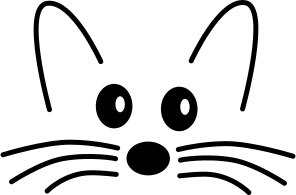
\includegraphics[width=1.4em]{squeak-logo}}}
\iftoshelse{
	\usepackage{marginnote}
		\renewcommand*{\marginfont}{\footnotesize}
	\newcommand{\vartriangleout}{\ifthenelse{\isodd{\thepage}}{\vartriangleright}{\vartriangleleft}}
	\newcommand{\dothisicon}{\fcolorbox{blue!65}{white}{\highlight{$\vartriangleout$}}}
	\newcommand{\dothis}[1]{%
		\noindent\par\noindent
		{\reversemarginpar
			\marginnote{\fcolorbox{blue!65}{white}{\highlight{$\vartriangleout$}}}}
		%\MarginLabel{do this}
		\noindent\emph{#1}
		\nopagebreak}
}{
	\newcommand{\dothisicon}{\raisebox{-.5ex}{
\includegraphics[height=1.2em]{pharo}}}
	\newcommand{\dothis}[1]{%
		\medskip
		\noindent\dothisicon
		\ifx#1\empty\else\quad\emph{#1}\fi
		\par\smallskip\nopagebreak}
}
%===> NEW VERSION <===
% NB: To use this in an individual chapter, you must set:
%\graphicspath{{figures/} {../figures/}}
% at the head of the chapter.  Don't forget the final /
%=============================================================
%:Reader hints (hint)
%
% Indicates a non-obvious consequence 
\newcommand{\hint}[1]{\vspace{1ex}\noindent\fbox{\textsc{Hint}} \emph{#1}}
%=================================================================
% graphics for Morphic handles
\newcommand{\grabHandle}{\raisebox{-0.2ex}{
\includegraphics[width=1em]{blackHandle}}}
\newcommand{\moveHandle}{\raisebox{-0.2ex}{
\includegraphics[width=1em]{moveHandle}}}
\newcommand{\debugHandle}{\raisebox{-0.2ex}{
\includegraphics[width=1em]{debugHandle}}}
%=============================================================
%:Highlighting Important stuff (doublebox)
%
% From Seaside book ...
\newsavebox{\SavedText}
\newlength{\InnerBoxRule}\setlength{\InnerBoxRule}{.75\fboxrule}
\newlength{\OuterBoxRule}\setlength{\OuterBoxRule}{1.5\fboxrule}
\newlength{\BoxSeparation}\setlength{\BoxSeparation}{1.5\fboxrule}
\addtolength{\BoxSeparation}{.5pt}
\newlength{\SaveBoxSep}\setlength{\SaveBoxSep}{2\fboxsep}
%
\newenvironment{doublebox}{\begin{lrbox}{\SavedText}
    \begin{minipage}{.75\textwidth}}
    {\end{minipage}\end{lrbox}\begin{center}
    \setlength{\fboxsep}{\BoxSeparation}\setlength{\fboxrule}{\OuterBoxRule}
    \fbox{\setlength{\fboxsep}{\SaveBoxSep}\setlength{\fboxrule}{\InnerBoxRule}%
      \fbox{\usebox{\SavedText}}}
  \end{center}}
% Use this:
\newcommand{\important}[1]{\begin{doublebox}#1\end{doublebox}}
%=============================================================
%:Section depth
\setcounter{secnumdepth}{2}
%% for this to happen start the file with
%\ifx\wholebook\relax\else
%% $Author$
% $Date$
% $Revision$

% HISTORY:
% 2006-10-31 - Oscar code macros
% ...

%=============================================================
% NB: documentclass must be set in main document.
% Allows book to be generated in multiple formats.
%=============================================================
%:Packages
\usepackage[T1]{fontenc}  %%%%%% really important to get the code directly in the text!
\usepackage{lmodern}
%\usepackage[scaled=0.85]{bookmanx} % needs another scale factor if used with \renewcommand{\sfdefault}{cmbr}
\usepackage{palatino}
\usepackage[scaled=0.85]{helvet}
\usepackage[protrusion,expansion=false]{microtype}
\usepackage{graphicx}
\usepackage{theorem}
\usepackage[english]{babel}
%%% ON: pdfsync breaks the use of p{width} for tabular columns!
%%\ifdefined\usepdfsync\usepackage{pdfsync}\fi % Requires texlive 2007
%=============================================================
%:More packages
%Stef should check which ones are used!
%\usepackage{picinpar}
%\usepackage{layout}
%\usepackage{color}
%\usepackage{enum}
%\usepackage{a4wide}
% \usepackage{fancyhdr}
\usepackage{ifthen}
\usepackage{float}
\usepackage{longtable}
\usepackage{makeidx}
\usepackage[nottoc]{tocbibind}
\usepackage{multicol}
\usepackage{booktabs}	% book-style tables
\usepackage{topcapt}	% enables \topcaption
\usepackage{multirow}
\usepackage{tabularx}
%\usepackage[bottom]{footmisc}
\usepackage{xspace}
\usepackage{alltt}
\usepackage{amssymb,textcomp}
\usepackage[usenames,dvipsnames]{color}
%\usepackage{colortbl}
\usepackage[hang]{subfigure}\makeatletter\def\p@subfigure{\thefigure\,}\makeatother
\usepackage{rotating}
\usepackage{enumitem}	% apb: allows more control over tags in enumerations
\usepackage{verbatim}     % for comment environment
\usepackage{varioref}	% for page references that work
\labelformat{footnote}{\thechapter--#1} % to distinguish citations from jurabib
\usepackage{needspace}
\usepackage{isodateo} % enable \isodate
\usepackage[newparttoc]{titlesec}
\usepackage{titletoc}
\usepackage{wrapfig}
\usepackage[
	super,
	citefull=first,
	authorformat={allreversed,and},
	titleformat={commasep,italic}
]{jurabib} % citations as footnotes
\usepackage[
	colorlinks=true,
	linkcolor=black,
	urlcolor=black,
	citecolor=black
]{hyperref}   % should come last
%=============================================================
%:PDF version
%%\pdfminorversion=3 % Set PDF to 1.3 for Lulu
%=============================================================
%:URL style
\makeatletter
\def\url@leostyle{%
  \@ifundefined{selectfont}{\def\UrlFont{\sf}}{\def\UrlFont{\sffamily}}}
\makeatother
% Now actually use the newly defined style.
\urlstyle{leo}
%=============================================================
%:Booleans
\newboolean{lulu}
\setboolean{lulu}{false}
\newcommand{\ifluluelse}[2]{\ifthenelse{\boolean{lulu}}{#1}{#2}}
%=============================================================
%:Names
\newcommand{\SUnit}{SUnit\xspace}
\newcommand{\sunit}{SUnit\xspace}
\newcommand{\xUnit}{$x$Unit\xspace}
\newcommand{\JUnit}{JUnit\xspace}
\newcommand{\st}{Smalltalk\xspace}
\newcommand{\pharo}{Pharo\xspace} % Use this, not \Pharo
%\newcommand{\sqmap}{SqueakMap\xspace}
\newcommand{\squeak}{Squeak\xspace} % use this, not \Squeak or \sq
\newcommand{\sqsrc}{SqueakSource\xspace}
\newcommand{\sbe}{\url{http://SqueakByExample.org}\xspace}
\newcommand{\pharoweb}{\url{http://pharo-project.org}\xspace}
\newcommand{\pbe}{\url{http://PharoByExample.org}\xspace}
\newcommand{\sba}{\url{http://SquareBracketAssociates.org}\xspace}
\newcommand{\bam}{\lct{Bounc\-ing\-Atoms\-Morph}\xspace}
%=============================================================
%:Markup macros for proof-reading
\usepackage[normalem]{ulem} % for \sout
\usepackage{xcolor}
\newcommand{\ra}{$\rightarrow$}
\newcommand{\ugh}[1]{\textcolor{red}{\uwave{#1}}} % please rephrase
\newcommand{\ins}[1]{\textcolor{blue}{\uline{#1}}} % please insert
\newcommand{\del}[1]{\textcolor{red}{\sout{#1}}} % please delete
\newcommand{\chg}[2]{\textcolor{red}{\sout{#1}}{\ra}\textcolor{blue}{\uline{#2}}} % please change
%=============================================================
%:Editorial comment macros
%\newcommand{\nnbb}[2]{
%    % \fbox{\bfseries\sffamily\scriptsize#1}
%    \fcolorbox{gray}{yellow}{\bfseries\sffamily\scriptsize#1}
%    {\sf\small$\blacktriangleright$\textit{#2}$\blacktriangleleft$}
%   }
\newcommand{\yellowbox}[1]{\fcolorbox{gray}{yellow}{\bfseries\sffamily\scriptsize#1}}
\newcommand{\triangles}[1]{{\sf\small$\blacktriangleright$\textit{#1}$\blacktriangleleft$}}
\newcommand{\nnbb}[2]{\yellowbox{#1} \triangles{#2}}
\newcommand{\fix}{\yellowbox{FIX!}}
\newcommand{\here}{\yellowbox{CONTINUE HERE!}}
% editor macros
\newcommand{\apl}[1]{\nnbb{Alain}{#1}} % Alain
\newcommand{\ab}[1]{\nnbb{Andrew}{#1}} % Black
\newcommand{\sd}[1]{\nnbb{St\'{e}f}{#1}} % Ducasse
\newcommand{\dc}[1]{\nnbb{DamienC}{#1}} % Ducasse
\newcommand{\md}[1]{\nnbb{Marcus}{#1}} % Denker
\newcommand{\on}[1]{\nnbb{Oscar}{#1}} % Nierstrasz
\newcommand{\damien}[1]{\nnbb{Damien}{#1}} % Pollet
\newcommand{\lr}[1]{\nnbb{Lukas}{#1}} % Renggli
\newcommand{\orla}[1]{\nnbb{Orla}{#1}} % Greevy
\newcommand{\alex}[1]{\nnbb{Alex}{#1}} % Bergel
\newcommand{\alx}[1]{\nnbb{Alex}{#1}} % Bergel
\newcommand{\dr}[1]{\nnbb{David}{#1}} % Roethlisberger
\newcommand{\ja}[1]{\nnbb{Jannik}{#1}} % Laval
\newcommand{\jr}[1]{\nnbb{Jorge}{#1}} % Ressia
\newcommand{\fp}[1]{\nnbb{Fabrizio}{#1}} % Perin
\newcommand{\michael}[1]{\nnbb{Michael}{#1}} % Davies
\newcommand{\ew}[1]{\nnbb{Erwann}{#1}} % Wernli
\newcommand{\mb}[1]{\nnbb{Martial}{#1}} % Boniou
\newcommand{\hw}[1]{\nnbb{Hernan}{#1}} % Wilkinson
%=============================================================
%:Abbreviation macros
\newcommand{\ie}{\emph{すなわち}、}
\newcommand{\eg}{\emph{例えば}、}
\newcommand{\etc}{などなど。}
%=============================================================
%:Cross reference macros
\newcommand{\charef}[1]{第~\ref{cha:#1}~章}
\newcommand{\secref}[1]{\ref{sec:#1}~節}
\newcommand{\figref}[1]{図~\ref{fig:#1}\xspace}
\newcommand{\Figref}[1]{図~\ref{fig:#1}\xspace}
\newcommand{\appref}[1]{付録~\ref{app:#1}\xspace}
\newcommand{\tabref}[1]{表~\ref{tab:#1}\xspace}
\newcommand{\faqref}[1]{FAQ~\ref{faq:#1}, p.~\pageref{faq:#1}\xspace}
% APB: I removed trailing \xspace commands from these macros because
% \xspace mostly doesn't work.  If you want a space after your
% references, type one!
% ON: xspace has always worked just fine for me!  Please leave them in.
%
\newcommand{\ruleref}[1]{\ref{rule:#1}\xspace}
%
\newcommand{\egref}[1]{example~\ref{eg:#1}\xspace}
\newcommand{\Egref}[1]{Example~\ref{eg:#1}\xspace}
%
\newcommand{\scrref}[1]{script~\ref{scr:#1}\xspace}
\newcommand{\Scrref}[1]{Script~\ref{scr:#1}\xspace}
\newcommand{\tscrref}[1]{the script~\ref{scr:#1}\xspace}
\newcommand{\Tscrref}[1]{The script~\ref{scr:#1}\xspace}
%
\newcommand{\mthref}[1]{method~\ref{mth:#1}\xspace}
\newcommand{\mthsref}[1]{methods~\ref{mth:#1}\xspace}
\newcommand{\Mthref}[1]{Method~\ref{mth:#1}\xspace}
\newcommand{\tmthref}[1]{the method~\ref{mth:#1}\xspace}
\newcommand{\Tmthref}[1]{The method~\ref{mth:#1}\xspace}
%
\newcommand{\clsref}[1]{class~\ref{cls:#1}\xspace}
\newcommand{\tclsref}[1]{the class~\ref{cls:#1}\xspace}
\newcommand{\Tclsref}[1]{The class~\ref{cls:#1}\xspace}

\newcommand{\chalabel}[1]{\label{cha:#1}}
\newcommand{\seclabel}[1]{\label{sec:#1}}
\newcommand{\figlabel}[1]{\label{fig:#1}}
\newcommand{\tablabel}[1]{\label{tab:#1}}
\newcommand{\rulelabel}[1]{\label{rule:#1}}
\newcommand{\eglabel}[1]{\label{eg:#1}}
\newcommand{\scrlabel}[1]{\label{scr:#1}}
\newcommand{\mthlabel}[1]{\label{mth:#1}}
\newcommand{\clslabel}[1]{\label{cls:#1}}
\newcommand{\faqlabel}[1]{\label{faq:#1}}
%=============================================================
%:Menu item macro
% for menu items, so we can change our minds on how to print them! (apb)
\definecolor{lightgray}{gray}{0.89}
\newcommand{\menu}[1]{{%
	\setlength{\fboxsep}{0pt}%
	\colorbox{lightgray}{{{\upshape\sffamily\strut \,#1\,}}}}}
\newcommand{\link}[1]{{%
	\fontfamily{lmr}\selectfont
 	\upshape{\sffamily \underline{#1}}}}
% For submenu items:
\newcommand{\go}{\,$\triangleright$\,}
% \newcommand{\go}{\,$\blacktriangleright$\,}
% For keyboard shortcuts:
%\newcommand{\short}[1]{\mbox{$\langle${\sc CMD}$\rangle$-#1}\xspace}
\newcommand{\short}[1]{\mbox{{\sc cmd}\hspace{0.08em}--\hspace{0.09em}#1}\xspace}
% For buttons:
\newcommand{\button}[1]{{%
	\setlength{\fboxsep}{0pt}%
	\fbox{{\upshape\sffamily\strut \,#1\,}}}}
% NB: The button macro does not work within captions -- incompatible with xcolor package :-(
\newcommand{\toolsflap}{\textit{Tools} flap\xspace}
%=============================================================
%:Mouse clicks
\newcommand{\click}{click\xspace} % RED
\newcommand{\actclick}{action-click\xspace} % YELLOW
\newcommand{\metaclick}{meta-click\xspace} % BLUE
\newcommand{\Click}{Click\xspace} % RED
\newcommand{\Actclick}{Action-click\xspace} % YELLOW
\newcommand{\Metaclick}{Meta-click\xspace} % BLUE
%=============================================================
%:ToSh macros
\newboolean{tosh}
\setboolean{tosh}{false}
\newcommand{\iftoshelse}[2]{\ifthenelse{\boolean{tosh}}{#1}{#2}}
%=============================================================
%:ToSh colors
%\newcommand{\highlightcolor}{\color{blue!65}}
%\newcommand{\boxcolor}{\color{gray!25}}
\newcommand{\highlight}[1]{\textcolor{blue!65}{#1}}
%\newcommand{\codecolor}{\color{blue!65}}
%%\setlength{\fboxrule}{2pt}
%\newcommand{\asPict}[1]{%
%	{\Large\highlight{#1}}}
%=============================================================
%:Reader cues (do this)
%
% Indicate something the reader should try out.
% \newcommand{\dothisicon}{\raisebox{-.5ex}{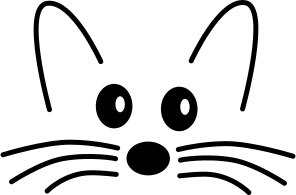
\includegraphics[width=1.4em]{squeak-logo}}}
\iftoshelse{
	\usepackage{marginnote}
		\renewcommand*{\marginfont}{\footnotesize}
	\newcommand{\vartriangleout}{\ifthenelse{\isodd{\thepage}}{\vartriangleright}{\vartriangleleft}}
	\newcommand{\dothisicon}{\fcolorbox{blue!65}{white}{\highlight{$\vartriangleout$}}}
	\newcommand{\dothis}[1]{%
		\noindent\par\noindent
		{\reversemarginpar
			\marginnote{\fcolorbox{blue!65}{white}{\highlight{$\vartriangleout$}}}}
		%\MarginLabel{do this}
		\noindent\emph{#1}
		\nopagebreak}
}{
	\newcommand{\dothisicon}{\raisebox{-.5ex}{
\includegraphics[height=1.2em]{pharo}}}
	\newcommand{\dothis}[1]{%
		\medskip
		\noindent\dothisicon
		\ifx#1\empty\else\quad\emph{#1}\fi
		\par\smallskip\nopagebreak}
}
%===> NEW VERSION <===
% NB: To use this in an individual chapter, you must set:
%\graphicspath{{figures/} {../figures/}}
% at the head of the chapter.  Don't forget the final /
%=============================================================
%:Reader hints (hint)
%
% Indicates a non-obvious consequence 
\newcommand{\hint}[1]{\vspace{1ex}\noindent\fbox{\textsc{Hint}} \emph{#1}}
%=================================================================
% graphics for Morphic handles
\newcommand{\grabHandle}{\raisebox{-0.2ex}{
\includegraphics[width=1em]{blackHandle}}}
\newcommand{\moveHandle}{\raisebox{-0.2ex}{
\includegraphics[width=1em]{moveHandle}}}
\newcommand{\debugHandle}{\raisebox{-0.2ex}{
\includegraphics[width=1em]{debugHandle}}}
%=============================================================
%:Highlighting Important stuff (doublebox)
%
% From Seaside book ...
\newsavebox{\SavedText}
\newlength{\InnerBoxRule}\setlength{\InnerBoxRule}{.75\fboxrule}
\newlength{\OuterBoxRule}\setlength{\OuterBoxRule}{1.5\fboxrule}
\newlength{\BoxSeparation}\setlength{\BoxSeparation}{1.5\fboxrule}
\addtolength{\BoxSeparation}{.5pt}
\newlength{\SaveBoxSep}\setlength{\SaveBoxSep}{2\fboxsep}
%
\newenvironment{doublebox}{\begin{lrbox}{\SavedText}
    \begin{minipage}{.75\textwidth}}
    {\end{minipage}\end{lrbox}\begin{center}
    \setlength{\fboxsep}{\BoxSeparation}\setlength{\fboxrule}{\OuterBoxRule}
    \fbox{\setlength{\fboxsep}{\SaveBoxSep}\setlength{\fboxrule}{\InnerBoxRule}%
      \fbox{\usebox{\SavedText}}}
  \end{center}}
% Use this:
\newcommand{\important}[1]{\begin{doublebox}#1\end{doublebox}}
%=============================================================
%:Section depth
\setcounter{secnumdepth}{2}
%% for this to happen start the file with
%\ifx\wholebook\relax\else
%\input{../common.tex}
%\begin{document}
%\fi
% and terminate by
% \ifx\wholebook\relax\else\end{document}\fi

\DeclareGraphicsExtensions{.pdf, .jpg, .png}
%=============================================================
%:PDF setup
\hypersetup{
%   a4paper,
%   pdfstartview=FitV,
%   colorlinks,
%   linkcolor=darkblue,
%   citecolor=darkblue,
   pdftitle={Pharo by Example},
   pdfauthor={Andrew P. Black, St\'ephane Ducasse,	Oscar Nierstrasz,
Damien Pollet},
   pdfkeywords={Smalltalk, Squeak, Object-Oriented Programming, OOP},
   pdfsubject={Computer Science}
}
%=============================================================
%:Page layout and appearance
%
% \renewcommand{\headrulewidth}{0pt}
\renewcommand{\chaptermark}[1]{\markboth{#1}{}}
\renewcommand{\sectionmark}[1]{\markright{\thesection\ #1}}
\renewpagestyle{plain}[\small\itshape]{%
	\setheadrule{0pt}%
	\sethead[][][]{}{}{}%
	\setfoot[][][]{}{}{}}
\renewpagestyle{headings}[\small\itshape]{%
	\setheadrule{0pt}%
	\setmarks{chapter}{section}%
	\sethead[\thepage][][\chaptertitle]{\sectiontitle}{}{\thepage}%
	\setfoot[][][]{}{}{}}
%=============================================================
%:Title section setup and TOC numbering depth
\setcounter{secnumdepth}{1}
\setcounter{tocdepth}{1}
\titleformat{\part}[display]{\centering}{\huge\partname\ \thepart}{1em}{\Huge\textbf}[]
\titleformat{\chapter}[display]{}{\huge\chaptertitlename\ \thechapter}{1em}{\Huge\raggedright\textbf}[]
\titlecontents{part}[3pc]{%
		\pagebreak[2]\addvspace{1em plus.4em minus.2em}%
		\leavevmode\large\bfseries}
	{\contentslabel{3pc}}{\hspace*{-3pc}}
	{}[\nopagebreak]
\titlecontents{chapter}[3pc]{%
		\pagebreak[0]\addvspace{1em plus.2em minus.2em}%
		\leavevmode\bfseries}
	{\contentslabel{3pc}}{}
	{\hfill\contentspage}[\nopagebreak]
\dottedcontents{section}[3pc]{}{3pc}{1pc}
\dottedcontents{subsection}[3pc]{}{0pc}{1pc}
% \dottedcontents{subsection}[4.5em]{}{0pt}{1pc}
% Make \cleardoublepage insert really blank pages http://www.tex.ac.uk/cgi-bin/texfaq2html?label=reallyblank
\let\origdoublepage\cleardoublepage
\newcommand{\clearemptydoublepage}{%
  \clearpage
  {\pagestyle{empty}\origdoublepage}}
\let\cleardoublepage\clearemptydoublepage % see http://www.tex.ac.uk/cgi-bin/texfaq2html?label=patch
%=============================================================
%:FAQ macros (for FAQ chapter)
\newtheorem{faq}{FAQ}
\newcommand{\answer}{\paragraph{Answer}\ }
%=============================================================
%:Listings package configuration
% \newcommand{\caret}{\makebox{\raisebox{0.4ex}{\footnotesize{$\wedge$}}}}
\newcommand{\caret}{\^\,}
\newcommand{\escape}{{\sf \textbackslash}}
\definecolor{source}{gray}{0.95}
\usepackage{listings}
\lstdefinelanguage{Smalltalk}{
%  morekeywords={self,super,true,false,nil,thisContext}, % This is overkill
  morestring=[d]',
  morecomment=[s]{"}{"},
  alsoletter={\#:},
  escapechar={!},
  literate=
    {BANG}{!}1
    {CARET}{\^}1
    {UNDERSCORE}{\_}1
    {\\st}{Smalltalk}9 % convenience -- in case \st occurs in code
    % {'}{{\textquotesingle}}1 % replaced by upquote=true in \lstset
    {_}{{$\leftarrow$}}1
    {>>>}{{\sep}}1
    {^}{{$\uparrow$}}1
    {~}{{$\sim$}}1
    {-}{{\texttt{-}}}1 %{\textminus}}1 %{-}{\hspace{-0.13em}}{-}}1  % the goal is to make - the same width as +
    % {+}{\sf+}1 %{\raisebox{0.08ex}{+}}}1      % and to raise + off the baseline to match -
    {-->}{{\quad$\longrightarrow$\quad}}3
	, % Don't forget the comma at the end!
  tabsize=4
}[keywords,comments,strings]

\lstset{language=Smalltalk,
	basicstyle=\sffamily,
	keywordstyle=\color{black}\bfseries,
	% stringstyle=\ttfamily, % Ugly! do we really want this? -- on
	mathescape=true,
	showstringspaces=false,
	keepspaces=true,
	breaklines=true,
	breakautoindent=true,
	backgroundcolor=\color{source},
	lineskip={-1pt}, % Ugly hack
	upquote=true, % straight quote; requires textcomp package
	columns=fullflexible} % no fixed width fonts
% In-line code (literal)
% Normally use this for all in-line code:
\newcommand{\ct}{\lstinline[mathescape=false,backgroundcolor=\color{white},basicstyle={\sffamily\upshape}]}
% apb 2007.8.28 added the \upshape declaration to avoid getting italicized code in \dothis{ } sections.
% In-line code (latex enabled)
% Use this only in special situations where \ct does not work
% (within section headings ...):
\newcommand{\lct}[1]{{\textsf{\textup{#1}}}}
% Use these for system categories and protocols:
\newcommand{\scat}[1]{\emph{\textsf{#1}}\xspace}
\newcommand{\pkg}[1]{\emph{\textsf{#1}}\xspace}
\newcommand{\prot}[1]{\emph{\textsf{#1}}\xspace}
% Code environments
% NB: the arg is for tests
% Only code and example environments may be tests
\lstnewenvironment{code}[1]{%
	\lstset{%
		% frame=lines,
		frame=single,
		framerule=0pt,
		mathescape=false
	}
}{}
\def\ignoredollar#1{}
%=============================================================
%:Code environments (method, script ...)
% NB: the third arg is for tests
% Only code and example environments may be tests
\lstnewenvironment{example}[3][defaultlabel]{%
	\renewcommand{\lstlistingname}{Example}%
	\lstset{
		% frame=lines,
		frame=single,
		framerule=0pt,
		mathescape=false,
		caption={\emph{#2}},
		label={eg:#1}
	}
}{}
\lstnewenvironment{script}[2][defaultlabel]{%
\renewcommand{\lstlistingname}{Script}%
	\lstset{
		% frame=lines,
		frame=single,
		framerule=0pt,
		mathescape=false,
		name={Script},
		caption={\emph{#2}},
		label={scr:#1}
	}
}{}
\lstnewenvironment{method}[2][defaultlabel]{%
	\renewcommand{\lstlistingname}{Method}%
	\lstset{
		% frame=lines,
		frame=single,
		framerule=0pt,
		mathescape=false,
		name={Method},
		caption={\emph{#2}},
		label={mth:#1}
	}
}{}
\lstnewenvironment{methods}[2][defaultlabel]{% just for multiple methods at once
	\renewcommand{\lstlistingname}{Methods}%
	\lstset{
		% frame=lines,
		frame=single,
		framerule=0pt,
		mathescape=false,
		name={Method},
		caption={\emph{#2}},
		label={mth:#1}
	}
}{}
\lstnewenvironment{numMethod}[2][defaultlabel]{%
	\renewcommand{\lstlistingname}{Method}%
	\lstset{
		numbers=left,
		numberstyle={\tiny\sffamily},
		% frame=lines,
		frame=single,
		framerule=0pt,
		mathescape=false,
		name={Method},
		caption={\emph{#2}},
		label={mth:#1}
	}
}{}
\lstnewenvironment{classdef}[2][defaultlabel]{%
	\renewcommand{\lstlistingname}{Class}%
	\lstset{
		% frame=lines,
		frame=single,
		framerule=0pt,
		mathescape=false,
		name={Class},
		caption={\emph{#2}},
		label={cls:#1}
	}
}{}
%=============================================================
%:Reserving space
% Usually need one more line than the actual lines of code
\newcommand{\needlines}[1]{\Needspace{#1\baselineskip}}
%=============================================================
%:Indexing macros
% Macros ending with "ind" generate text as well as an index entry
% Macros ending with "index" *only* generate an index entry
\newcommand{\ind}[1]{\index{#1}#1\xspace} % plain text
\newcommand{\subind}[2]{\index{#1!#2}#2\xspace} % show #2, subindex under #1
\newcommand{\emphind}[1]{\index{#1}\emph{#1}\xspace} % emph #1
\newcommand{\emphsubind}[2]{\index{#1!#2}\emph{#2}\xspace} % show emph #2, subindex inder #1
\newcommand{\scatind}[1]{\index{#1@\textsf{#1} (category)}\scat{#1}} % category
\newcommand{\pkgind}[1]{\index{#1@\textsf{#1} (package)}\pkg{#1}} % package
\newcommand{\protind}[1]{\index{#1@\textsf{#1} (protocol)}\prot{#1}} % protocol
\newcommand{\clsind}[1]{\index{#1@\textsf{#1} (class)}\ct{#1}\xspace}
% \newcommand{\clsind}[1]{\index{#1!\#@(class)}\ct{#1}\xspace} % class
\newcommand{\clsindplural}[1]{\index{#1!\#@(class)}\ct{#1}s\xspace} % class
\newcommand{\cvind}[1]{\index{#1@\textsf{#1} (class variable)}\ct{#1}\xspace} % class var
\newcommand{\glbind}[1]{\index{#1@\textsf{#1} (global)}\ct{#1}\xspace} % global
\newcommand{\patind}[1]{\index{#1@#1 (pattern)}\ct{#1}\xspace} % pattern
\newcommand{\pvind}[1]{\index{#1@\textsf{#1} (pseudo variable)}\ct{#1}\xspace} % pseudo var
\newcommand{\clsmthind}[2]{\index{#1!#2@\ct{#2}}\ct{#1>>>#2}\xspace} % class + method name
\newcommand{\mthind}[2]{\index{#1!#2@\ct{#2}}\ct{#2}\xspace} % show method name only
\newcommand{\lmthind}[2]{\index{#1!#2@\ct{#2}}\lct{#2}\xspace} % show method name only
\newcommand{\cmind}[2]{\index{#1!#2@\ct{#2}}\ct{#1>>>#2}\xspace} % show class>>method
\newcommand{\lcmind}[2]{\index{#1!#2@\ct{#2}}\lct{#1>>>#2}\xspace} % show class>>method
\newcommand{\toolsflapind}{\index{Tools flap}\toolsflap} % index tools flap
% The following only generate an index entry:
% \newcommand{\clsindex}[1]{\index{#1@\textsf{#1} (class)}}
\newcommand{\clsindex}[1]{\index{#1!\#@(class)}} % class
\newcommand{\mthindex}[2]{\index{#1!#2@\ct{#2}}} % method
\newcommand{\cmindex}[2]{\index{#1!#2@\ct{#2}}} % class>>method
\newcommand{\cvindex}[1]{\index{#1@\textsf{#1} (class variable)}} % class var
\newcommand{\glbindex}[1]{\index{#1@\textsf{#1} (global)}}% global
\newcommand{\pvindex}[1]{\index{#1@\textsf{#1} (pseudo variable)}}% pseudo var
\newcommand{\seeindex}[2]{\index{#1|see{#2}}} % #1, see #2
\newcommand{\scatindex}[1]{\index{#1@\textsf{#1} (category)}} % category
\newcommand{\pkgindex}[1]{\index{#1@\textsf{#1} (package)}} % package
\newcommand{\protindex}[1]{\index{#1@\textsf{#1} (protocol)}} % protocol
% How can we have the main entry page numbers in bold yet not break the hyperlink?
\newcommand{\boldidx}[1]{{\bf #1}} % breaks hyperlink
%\newcommand{\indmain}[1]{\index{#1|boldidx}#1\xspace} % plain text, main entry
%\newcommand{\emphsubindmain}[2]{\index{#1!#2|boldidx}\emph{#2}\xspace} % subindex, main entry
%\newcommand{\subindmain}[2]{\index{#1!#2|boldidx}#2\xspace} % subindex, main entry
%\newcommand{\clsindmain}[1]{\index{#1@\textsf{#1} (class)|boldidx}\ct{#1}\xspace}
%\newcommand{\clsindmain}[1]{\index{#1!\#@(class)|boldidx}\ct{#1}\xspace} % class main
%\newcommand{\indexmain}[1]{\index{#1|boldidx}} % main index entry only
\newcommand{\indmain}[1]{\index{#1}#1\xspace} % The main index entry for this item
\newcommand{\emphsubindmain}[2]{\index{#1!#2}\emph{#2}\xspace} % subindex, main entry
\newcommand{\subindmain}[2]{\index{#1!#2}#2\xspace} % subindex, main entry
%\newcommand{\clsindmain}[1]{\index{#1@\textsf{#1} (class)}\ct{#1}\xspace}
\newcommand{\clsindmain}[1]{\index{#1!\#@(class)}\ct{#1}\xspace} % class main
\newcommand{\clsindexmain}[1]{\index{#1!\#@(class)}} % class main index only
\newcommand{\indexmain}[1]{\index{#1}} 
%=============================================================
%:Code macros
% some constants
\newcommand{\codesize}{\small}
\newcommand{\codefont}{\sffamily}
%\newcommand{\cat}[1]{\textit{In category #1}}%%To remove later
\newlength{\scriptindent}
\setlength{\scriptindent}{.3cm}
%% Method presentation constants
\newlength{\methodindent}
\newlength{\methodwordlength}
\newlength{\aftermethod}
\setlength{\methodindent}{0.2cm}
\settowidth{\methodwordlength}{\ M\'ethode\ }
%=============================================================
%:Smalltalk macros
%\newcommand{\sep}{{$\gg$}}
\newcommand{\sep}{\mbox{>>}}
\newcommand{\self}{\lct{self}\xspace}
\newcommand{\super}{\lct{super}\xspace}
\newcommand{\nil}{\lct{nil}\xspace}
%=============================================================
% be less conservative about float placement
% these commands are from http://www.tex.ac.uk/cgi-bin/texfaq2html?label=floats
\renewcommand{\topfraction}{.9}
\renewcommand{\bottomfraction}{.9}
\renewcommand{\textfraction}{.1}
\renewcommand{\floatpagefraction}{.85}
\renewcommand{\dbltopfraction}{.66}
\renewcommand{\dblfloatpagefraction}{.85}
\setcounter{topnumber}{9}
\setcounter{bottomnumber}{9}
\setcounter{totalnumber}{20}
\setcounter{dbltopnumber}{9}
%=============================================================
% Give information from each chapter's author
\newcommand{\contact}[2]{\textbf{#1} \textsf{(#2)}}

\newcommand{\chapterauthor}[1]{\emph{with the participation of:\\#1}\\}

\newcommand{\authornoury}{\contact{Noury Bouraqadi}{bouraqadi@gmail.com}}
\newcommand{\authordamienc}{\contact{Damien Cassou}{damien.cassou@gmail.com}}
\newcommand{\authoroscar}{\contact{Oscar Nierstrasz}{oscar.nierstrasz@acm.org}}
\newcommand{\authorsteph}{\contact{St\'ephane Ducasse}{stephane.ducasse@inria.fr}}
\newcommand{\authoralex}{\contact{Alexandre Bergel}{alexandre@bergel.eu}}
\newcommand{\authorolivier}{\contact{Olivier Auverlot}{olivier.auverlot@inria.fr}}
\newcommand{\authornicolas}{\contact{Nicolas Cellier}{ncellier@ifrance.com}}
\newcommand{\authormarcus}{\contact{Marcus Denker}{marcus.denker@inria.fr}}
\newcommand{\authoralain}{\contact{Alain Plantec}{alain.plantec@univ-brest.fr}}
\newcommand{\authordale}{\contact{Dale Henrichs}{dale.henrichs@gemstone.com}}
\newcommand{\authormariano}{\contact{Mariano Martinez Peck}{marianopeck@gmail.com}}
\newcommand{\authorsven}{\contact{Sven Van Caekenberghe}{sven@beta9.be}}

%=============================================================
% apb doesn't like paragraphs to run in to each other without a break
\parskip 1ex
%=============================================================
%:Stuff to check, merge or deprecate
%\setlength{\marginparsep}{2mm}
%\renewcommand{\baselinestretch}{1.1}
%=============================================================

%\begin{document}
%\fi
% and terminate by
% \ifx\wholebook\relax\else\end{document}\fi

\DeclareGraphicsExtensions{.pdf, .jpg, .png}
%=============================================================
%:PDF setup
\hypersetup{
%   a4paper,
%   pdfstartview=FitV,
%   colorlinks,
%   linkcolor=darkblue,
%   citecolor=darkblue,
   pdftitle={Pharo by Example},
   pdfauthor={Andrew P. Black, St\'ephane Ducasse,	Oscar Nierstrasz,
Damien Pollet},
   pdfkeywords={Smalltalk, Squeak, Object-Oriented Programming, OOP},
   pdfsubject={Computer Science}
}
%=============================================================
%:Page layout and appearance
%
% \renewcommand{\headrulewidth}{0pt}
\renewcommand{\chaptermark}[1]{\markboth{#1}{}}
\renewcommand{\sectionmark}[1]{\markright{\thesection\ #1}}
\renewpagestyle{plain}[\small\itshape]{%
	\setheadrule{0pt}%
	\sethead[][][]{}{}{}%
	\setfoot[][][]{}{}{}}
\renewpagestyle{headings}[\small\itshape]{%
	\setheadrule{0pt}%
	\setmarks{chapter}{section}%
	\sethead[\thepage][][\chaptertitle]{\sectiontitle}{}{\thepage}%
	\setfoot[][][]{}{}{}}
%=============================================================
%:Title section setup and TOC numbering depth
\setcounter{secnumdepth}{1}
\setcounter{tocdepth}{1}
\titleformat{\part}[display]{\centering}{\huge\partname\ \thepart}{1em}{\Huge\textbf}[]
\titleformat{\chapter}[display]{}{\huge\chaptertitlename\ \thechapter}{1em}{\Huge\raggedright\textbf}[]
\titlecontents{part}[3pc]{%
		\pagebreak[2]\addvspace{1em plus.4em minus.2em}%
		\leavevmode\large\bfseries}
	{\contentslabel{3pc}}{\hspace*{-3pc}}
	{}[\nopagebreak]
\titlecontents{chapter}[3pc]{%
		\pagebreak[0]\addvspace{1em plus.2em minus.2em}%
		\leavevmode\bfseries}
	{\contentslabel{3pc}}{}
	{\hfill\contentspage}[\nopagebreak]
\dottedcontents{section}[3pc]{}{3pc}{1pc}
\dottedcontents{subsection}[3pc]{}{0pc}{1pc}
% \dottedcontents{subsection}[4.5em]{}{0pt}{1pc}
% Make \cleardoublepage insert really blank pages http://www.tex.ac.uk/cgi-bin/texfaq2html?label=reallyblank
\let\origdoublepage\cleardoublepage
\newcommand{\clearemptydoublepage}{%
  \clearpage
  {\pagestyle{empty}\origdoublepage}}
\let\cleardoublepage\clearemptydoublepage % see http://www.tex.ac.uk/cgi-bin/texfaq2html?label=patch
%=============================================================
%:FAQ macros (for FAQ chapter)
\newtheorem{faq}{FAQ}
\newcommand{\answer}{\paragraph{Answer}\ }
%=============================================================
%:Listings package configuration
% \newcommand{\caret}{\makebox{\raisebox{0.4ex}{\footnotesize{$\wedge$}}}}
\newcommand{\caret}{\^\,}
\newcommand{\escape}{{\sf \textbackslash}}
\definecolor{source}{gray}{0.95}
\usepackage{listings}
\lstdefinelanguage{Smalltalk}{
%  morekeywords={self,super,true,false,nil,thisContext}, % This is overkill
  morestring=[d]',
  morecomment=[s]{"}{"},
  alsoletter={\#:},
  escapechar={!},
  literate=
    {BANG}{!}1
    {CARET}{\^}1
    {UNDERSCORE}{\_}1
    {\\st}{Smalltalk}9 % convenience -- in case \st occurs in code
    % {'}{{\textquotesingle}}1 % replaced by upquote=true in \lstset
    {_}{{$\leftarrow$}}1
    {>>>}{{\sep}}1
    {^}{{$\uparrow$}}1
    {~}{{$\sim$}}1
    {-}{{\texttt{-}}}1 %{\textminus}}1 %{-}{\hspace{-0.13em}}{-}}1  % the goal is to make - the same width as +
    % {+}{\sf+}1 %{\raisebox{0.08ex}{+}}}1      % and to raise + off the baseline to match -
    {-->}{{\quad$\longrightarrow$\quad}}3
	, % Don't forget the comma at the end!
  tabsize=4
}[keywords,comments,strings]

\lstset{language=Smalltalk,
	basicstyle=\sffamily,
	keywordstyle=\color{black}\bfseries,
	% stringstyle=\ttfamily, % Ugly! do we really want this? -- on
	mathescape=true,
	showstringspaces=false,
	keepspaces=true,
	breaklines=true,
	breakautoindent=true,
	backgroundcolor=\color{source},
	lineskip={-1pt}, % Ugly hack
	upquote=true, % straight quote; requires textcomp package
	columns=fullflexible} % no fixed width fonts
% In-line code (literal)
% Normally use this for all in-line code:
\newcommand{\ct}{\lstinline[mathescape=false,backgroundcolor=\color{white},basicstyle={\sffamily\upshape}]}
% apb 2007.8.28 added the \upshape declaration to avoid getting italicized code in \dothis{ } sections.
% In-line code (latex enabled)
% Use this only in special situations where \ct does not work
% (within section headings ...):
\newcommand{\lct}[1]{{\textsf{\textup{#1}}}}
% Use these for system categories and protocols:
\newcommand{\scat}[1]{\emph{\textsf{#1}}\xspace}
\newcommand{\pkg}[1]{\emph{\textsf{#1}}\xspace}
\newcommand{\prot}[1]{\emph{\textsf{#1}}\xspace}
% Code environments
% NB: the arg is for tests
% Only code and example environments may be tests
\lstnewenvironment{code}[1]{%
	\lstset{%
		% frame=lines,
		frame=single,
		framerule=0pt,
		mathescape=false
	}
}{}
\def\ignoredollar#1{}
%=============================================================
%:Code environments (method, script ...)
% NB: the third arg is for tests
% Only code and example environments may be tests
\lstnewenvironment{example}[3][defaultlabel]{%
	\renewcommand{\lstlistingname}{Example}%
	\lstset{
		% frame=lines,
		frame=single,
		framerule=0pt,
		mathescape=false,
		caption={\emph{#2}},
		label={eg:#1}
	}
}{}
\lstnewenvironment{script}[2][defaultlabel]{%
\renewcommand{\lstlistingname}{Script}%
	\lstset{
		% frame=lines,
		frame=single,
		framerule=0pt,
		mathescape=false,
		name={Script},
		caption={\emph{#2}},
		label={scr:#1}
	}
}{}
\lstnewenvironment{method}[2][defaultlabel]{%
	\renewcommand{\lstlistingname}{Method}%
	\lstset{
		% frame=lines,
		frame=single,
		framerule=0pt,
		mathescape=false,
		name={Method},
		caption={\emph{#2}},
		label={mth:#1}
	}
}{}
\lstnewenvironment{methods}[2][defaultlabel]{% just for multiple methods at once
	\renewcommand{\lstlistingname}{Methods}%
	\lstset{
		% frame=lines,
		frame=single,
		framerule=0pt,
		mathescape=false,
		name={Method},
		caption={\emph{#2}},
		label={mth:#1}
	}
}{}
\lstnewenvironment{numMethod}[2][defaultlabel]{%
	\renewcommand{\lstlistingname}{Method}%
	\lstset{
		numbers=left,
		numberstyle={\tiny\sffamily},
		% frame=lines,
		frame=single,
		framerule=0pt,
		mathescape=false,
		name={Method},
		caption={\emph{#2}},
		label={mth:#1}
	}
}{}
\lstnewenvironment{classdef}[2][defaultlabel]{%
	\renewcommand{\lstlistingname}{Class}%
	\lstset{
		% frame=lines,
		frame=single,
		framerule=0pt,
		mathescape=false,
		name={Class},
		caption={\emph{#2}},
		label={cls:#1}
	}
}{}
%=============================================================
%:Reserving space
% Usually need one more line than the actual lines of code
\newcommand{\needlines}[1]{\Needspace{#1\baselineskip}}
%=============================================================
%:Indexing macros
% Macros ending with "ind" generate text as well as an index entry
% Macros ending with "index" *only* generate an index entry
\newcommand{\ind}[1]{\index{#1}#1\xspace} % plain text
\newcommand{\subind}[2]{\index{#1!#2}#2\xspace} % show #2, subindex under #1
\newcommand{\emphind}[1]{\index{#1}\emph{#1}\xspace} % emph #1
\newcommand{\emphsubind}[2]{\index{#1!#2}\emph{#2}\xspace} % show emph #2, subindex inder #1
\newcommand{\scatind}[1]{\index{#1@\textsf{#1} (category)}\scat{#1}} % category
\newcommand{\pkgind}[1]{\index{#1@\textsf{#1} (package)}\pkg{#1}} % package
\newcommand{\protind}[1]{\index{#1@\textsf{#1} (protocol)}\prot{#1}} % protocol
\newcommand{\clsind}[1]{\index{#1@\textsf{#1} (class)}\ct{#1}\xspace}
% \newcommand{\clsind}[1]{\index{#1!\#@(class)}\ct{#1}\xspace} % class
\newcommand{\clsindplural}[1]{\index{#1!\#@(class)}\ct{#1}s\xspace} % class
\newcommand{\cvind}[1]{\index{#1@\textsf{#1} (class variable)}\ct{#1}\xspace} % class var
\newcommand{\glbind}[1]{\index{#1@\textsf{#1} (global)}\ct{#1}\xspace} % global
\newcommand{\patind}[1]{\index{#1@#1 (pattern)}\ct{#1}\xspace} % pattern
\newcommand{\pvind}[1]{\index{#1@\textsf{#1} (pseudo variable)}\ct{#1}\xspace} % pseudo var
\newcommand{\clsmthind}[2]{\index{#1!#2@\ct{#2}}\ct{#1>>>#2}\xspace} % class + method name
\newcommand{\mthind}[2]{\index{#1!#2@\ct{#2}}\ct{#2}\xspace} % show method name only
\newcommand{\lmthind}[2]{\index{#1!#2@\ct{#2}}\lct{#2}\xspace} % show method name only
\newcommand{\cmind}[2]{\index{#1!#2@\ct{#2}}\ct{#1>>>#2}\xspace} % show class>>method
\newcommand{\lcmind}[2]{\index{#1!#2@\ct{#2}}\lct{#1>>>#2}\xspace} % show class>>method
\newcommand{\toolsflapind}{\index{Tools flap}\toolsflap} % index tools flap
% The following only generate an index entry:
% \newcommand{\clsindex}[1]{\index{#1@\textsf{#1} (class)}}
\newcommand{\clsindex}[1]{\index{#1!\#@(class)}} % class
\newcommand{\mthindex}[2]{\index{#1!#2@\ct{#2}}} % method
\newcommand{\cmindex}[2]{\index{#1!#2@\ct{#2}}} % class>>method
\newcommand{\cvindex}[1]{\index{#1@\textsf{#1} (class variable)}} % class var
\newcommand{\glbindex}[1]{\index{#1@\textsf{#1} (global)}}% global
\newcommand{\pvindex}[1]{\index{#1@\textsf{#1} (pseudo variable)}}% pseudo var
\newcommand{\seeindex}[2]{\index{#1|see{#2}}} % #1, see #2
\newcommand{\scatindex}[1]{\index{#1@\textsf{#1} (category)}} % category
\newcommand{\pkgindex}[1]{\index{#1@\textsf{#1} (package)}} % package
\newcommand{\protindex}[1]{\index{#1@\textsf{#1} (protocol)}} % protocol
% How can we have the main entry page numbers in bold yet not break the hyperlink?
\newcommand{\boldidx}[1]{{\bf #1}} % breaks hyperlink
%\newcommand{\indmain}[1]{\index{#1|boldidx}#1\xspace} % plain text, main entry
%\newcommand{\emphsubindmain}[2]{\index{#1!#2|boldidx}\emph{#2}\xspace} % subindex, main entry
%\newcommand{\subindmain}[2]{\index{#1!#2|boldidx}#2\xspace} % subindex, main entry
%\newcommand{\clsindmain}[1]{\index{#1@\textsf{#1} (class)|boldidx}\ct{#1}\xspace}
%\newcommand{\clsindmain}[1]{\index{#1!\#@(class)|boldidx}\ct{#1}\xspace} % class main
%\newcommand{\indexmain}[1]{\index{#1|boldidx}} % main index entry only
\newcommand{\indmain}[1]{\index{#1}#1\xspace} % The main index entry for this item
\newcommand{\emphsubindmain}[2]{\index{#1!#2}\emph{#2}\xspace} % subindex, main entry
\newcommand{\subindmain}[2]{\index{#1!#2}#2\xspace} % subindex, main entry
%\newcommand{\clsindmain}[1]{\index{#1@\textsf{#1} (class)}\ct{#1}\xspace}
\newcommand{\clsindmain}[1]{\index{#1!\#@(class)}\ct{#1}\xspace} % class main
\newcommand{\clsindexmain}[1]{\index{#1!\#@(class)}} % class main index only
\newcommand{\indexmain}[1]{\index{#1}} 
%=============================================================
%:Code macros
% some constants
\newcommand{\codesize}{\small}
\newcommand{\codefont}{\sffamily}
%\newcommand{\cat}[1]{\textit{In category #1}}%%To remove later
\newlength{\scriptindent}
\setlength{\scriptindent}{.3cm}
%% Method presentation constants
\newlength{\methodindent}
\newlength{\methodwordlength}
\newlength{\aftermethod}
\setlength{\methodindent}{0.2cm}
\settowidth{\methodwordlength}{\ M\'ethode\ }
%=============================================================
%:Smalltalk macros
%\newcommand{\sep}{{$\gg$}}
\newcommand{\sep}{\mbox{>>}}
\newcommand{\self}{\lct{self}\xspace}
\newcommand{\super}{\lct{super}\xspace}
\newcommand{\nil}{\lct{nil}\xspace}
%=============================================================
% be less conservative about float placement
% these commands are from http://www.tex.ac.uk/cgi-bin/texfaq2html?label=floats
\renewcommand{\topfraction}{.9}
\renewcommand{\bottomfraction}{.9}
\renewcommand{\textfraction}{.1}
\renewcommand{\floatpagefraction}{.85}
\renewcommand{\dbltopfraction}{.66}
\renewcommand{\dblfloatpagefraction}{.85}
\setcounter{topnumber}{9}
\setcounter{bottomnumber}{9}
\setcounter{totalnumber}{20}
\setcounter{dbltopnumber}{9}
%=============================================================
% Give information from each chapter's author
\newcommand{\contact}[2]{\textbf{#1} \textsf{(#2)}}

\newcommand{\chapterauthor}[1]{\emph{with the participation of:\\#1}\\}

\newcommand{\authornoury}{\contact{Noury Bouraqadi}{bouraqadi@gmail.com}}
\newcommand{\authordamienc}{\contact{Damien Cassou}{damien.cassou@gmail.com}}
\newcommand{\authoroscar}{\contact{Oscar Nierstrasz}{oscar.nierstrasz@acm.org}}
\newcommand{\authorsteph}{\contact{St\'ephane Ducasse}{stephane.ducasse@inria.fr}}
\newcommand{\authoralex}{\contact{Alexandre Bergel}{alexandre@bergel.eu}}
\newcommand{\authorolivier}{\contact{Olivier Auverlot}{olivier.auverlot@inria.fr}}
\newcommand{\authornicolas}{\contact{Nicolas Cellier}{ncellier@ifrance.com}}
\newcommand{\authormarcus}{\contact{Marcus Denker}{marcus.denker@inria.fr}}
\newcommand{\authoralain}{\contact{Alain Plantec}{alain.plantec@univ-brest.fr}}
\newcommand{\authordale}{\contact{Dale Henrichs}{dale.henrichs@gemstone.com}}
\newcommand{\authormariano}{\contact{Mariano Martinez Peck}{marianopeck@gmail.com}}
\newcommand{\authorsven}{\contact{Sven Van Caekenberghe}{sven@beta9.be}}

%=============================================================
% apb doesn't like paragraphs to run in to each other without a break
\parskip 1ex
%=============================================================
%:Stuff to check, merge or deprecate
%\setlength{\marginparsep}{2mm}
%\renewcommand{\baselinestretch}{1.1}
%=============================================================

%\begin{document}
%\fi
% and terminate by
% \ifx\wholebook\relax\else\end{document}\fi

\DeclareGraphicsExtensions{.pdf, .jpg, .png}
%=============================================================
%:PDF setup
\hypersetup{
%   a4paper,
%   pdfstartview=FitV,
%   colorlinks,
%   linkcolor=darkblue,
%   citecolor=darkblue,
   pdftitle={Pharo by Example},
   pdfauthor={Andrew P. Black, St\'ephane Ducasse,	Oscar Nierstrasz,
Damien Pollet},
   pdfkeywords={Smalltalk, Squeak, Object-Oriented Programming, OOP},
   pdfsubject={Computer Science}
}
%=============================================================
%:Page layout and appearance
%
% \renewcommand{\headrulewidth}{0pt}
\renewcommand{\chaptermark}[1]{\markboth{#1}{}}
\renewcommand{\sectionmark}[1]{\markright{\thesection\ #1}}
\renewpagestyle{plain}[\small\itshape]{%
	\setheadrule{0pt}%
	\sethead[][][]{}{}{}%
	\setfoot[][][]{}{}{}}
\renewpagestyle{headings}[\small\itshape]{%
	\setheadrule{0pt}%
	\setmarks{chapter}{section}%
	\sethead[\thepage][][\chaptertitle]{\sectiontitle}{}{\thepage}%
	\setfoot[][][]{}{}{}}
%=============================================================
%:Title section setup and TOC numbering depth
\setcounter{secnumdepth}{1}
\setcounter{tocdepth}{1}
\titleformat{\part}[display]{\centering}{\huge\partname\ \thepart}{1em}{\Huge\textbf}[]
\titleformat{\chapter}[display]{}{\huge\chaptertitlename\ \thechapter}{1em}{\Huge\raggedright\textbf}[]
\titlecontents{part}[3pc]{%
		\pagebreak[2]\addvspace{1em plus.4em minus.2em}%
		\leavevmode\large\bfseries}
	{\contentslabel{3pc}}{\hspace*{-3pc}}
	{}[\nopagebreak]
\titlecontents{chapter}[3pc]{%
		\pagebreak[0]\addvspace{1em plus.2em minus.2em}%
		\leavevmode\bfseries}
	{\contentslabel{3pc}}{}
	{\hfill\contentspage}[\nopagebreak]
\dottedcontents{section}[3pc]{}{3pc}{1pc}
\dottedcontents{subsection}[3pc]{}{0pc}{1pc}
% \dottedcontents{subsection}[4.5em]{}{0pt}{1pc}
% Make \cleardoublepage insert really blank pages http://www.tex.ac.uk/cgi-bin/texfaq2html?label=reallyblank
\let\origdoublepage\cleardoublepage
\newcommand{\clearemptydoublepage}{%
  \clearpage
  {\pagestyle{empty}\origdoublepage}}
\let\cleardoublepage\clearemptydoublepage % see http://www.tex.ac.uk/cgi-bin/texfaq2html?label=patch
%=============================================================
%:FAQ macros (for FAQ chapter)
\newtheorem{faq}{FAQ}
\newcommand{\answer}{\paragraph{Answer}\ }
%=============================================================
%:Listings package configuration
% \newcommand{\caret}{\makebox{\raisebox{0.4ex}{\footnotesize{$\wedge$}}}}
\newcommand{\caret}{\^\,}
\newcommand{\escape}{{\sf \textbackslash}}
\definecolor{source}{gray}{0.95}
\usepackage{listings}
\lstdefinelanguage{Smalltalk}{
%  morekeywords={self,super,true,false,nil,thisContext}, % This is overkill
  morestring=[d]',
  morecomment=[s]{"}{"},
  alsoletter={\#:},
  escapechar={!},
  literate=
    {BANG}{!}1
    {CARET}{\^}1
    {UNDERSCORE}{\_}1
    {\\st}{Smalltalk}9 % convenience -- in case \st occurs in code
    % {'}{{\textquotesingle}}1 % replaced by upquote=true in \lstset
    {_}{{$\leftarrow$}}1
    {>>>}{{\sep}}1
    {^}{{$\uparrow$}}1
    {~}{{$\sim$}}1
    {-}{{\texttt{-}}}1 %{\textminus}}1 %{-}{\hspace{-0.13em}}{-}}1  % the goal is to make - the same width as +
    % {+}{\sf+}1 %{\raisebox{0.08ex}{+}}}1      % and to raise + off the baseline to match -
    {-->}{{\quad$\longrightarrow$\quad}}3
	, % Don't forget the comma at the end!
  tabsize=4
}[keywords,comments,strings]

\lstset{language=Smalltalk,
	basicstyle=\sffamily,
	keywordstyle=\color{black}\bfseries,
	% stringstyle=\ttfamily, % Ugly! do we really want this? -- on
	mathescape=true,
	showstringspaces=false,
	keepspaces=true,
	breaklines=true,
	breakautoindent=true,
	backgroundcolor=\color{source},
	lineskip={-1pt}, % Ugly hack
	upquote=true, % straight quote; requires textcomp package
	columns=fullflexible} % no fixed width fonts
% In-line code (literal)
% Normally use this for all in-line code:
\newcommand{\ct}{\lstinline[mathescape=false,backgroundcolor=\color{white},basicstyle={\sffamily\upshape}]}
% apb 2007.8.28 added the \upshape declaration to avoid getting italicized code in \dothis{ } sections.
% In-line code (latex enabled)
% Use this only in special situations where \ct does not work
% (within section headings ...):
\newcommand{\lct}[1]{{\textsf{\textup{#1}}}}
% Use these for system categories and protocols:
\newcommand{\scat}[1]{\emph{\textsf{#1}}\xspace}
\newcommand{\pkg}[1]{\emph{\textsf{#1}}\xspace}
\newcommand{\prot}[1]{\emph{\textsf{#1}}\xspace}
% Code environments
% NB: the arg is for tests
% Only code and example environments may be tests
\lstnewenvironment{code}[1]{%
	\lstset{%
		% frame=lines,
		frame=single,
		framerule=0pt,
		mathescape=false
	}
}{}
\def\ignoredollar#1{}
%=============================================================
%:Code environments (method, script ...)
% NB: the third arg is for tests
% Only code and example environments may be tests
\lstnewenvironment{example}[3][defaultlabel]{%
	\renewcommand{\lstlistingname}{Example}%
	\lstset{
		% frame=lines,
		frame=single,
		framerule=0pt,
		mathescape=false,
		caption={\emph{#2}},
		label={eg:#1}
	}
}{}
\lstnewenvironment{script}[2][defaultlabel]{%
\renewcommand{\lstlistingname}{Script}%
	\lstset{
		% frame=lines,
		frame=single,
		framerule=0pt,
		mathescape=false,
		name={Script},
		caption={\emph{#2}},
		label={scr:#1}
	}
}{}
\lstnewenvironment{method}[2][defaultlabel]{%
	\renewcommand{\lstlistingname}{Method}%
	\lstset{
		% frame=lines,
		frame=single,
		framerule=0pt,
		mathescape=false,
		name={Method},
		caption={\emph{#2}},
		label={mth:#1}
	}
}{}
\lstnewenvironment{methods}[2][defaultlabel]{% just for multiple methods at once
	\renewcommand{\lstlistingname}{Methods}%
	\lstset{
		% frame=lines,
		frame=single,
		framerule=0pt,
		mathescape=false,
		name={Method},
		caption={\emph{#2}},
		label={mth:#1}
	}
}{}
\lstnewenvironment{numMethod}[2][defaultlabel]{%
	\renewcommand{\lstlistingname}{Method}%
	\lstset{
		numbers=left,
		numberstyle={\tiny\sffamily},
		% frame=lines,
		frame=single,
		framerule=0pt,
		mathescape=false,
		name={Method},
		caption={\emph{#2}},
		label={mth:#1}
	}
}{}
\lstnewenvironment{classdef}[2][defaultlabel]{%
	\renewcommand{\lstlistingname}{Class}%
	\lstset{
		% frame=lines,
		frame=single,
		framerule=0pt,
		mathescape=false,
		name={Class},
		caption={\emph{#2}},
		label={cls:#1}
	}
}{}
%=============================================================
%:Reserving space
% Usually need one more line than the actual lines of code
\newcommand{\needlines}[1]{\Needspace{#1\baselineskip}}
%=============================================================
%:Indexing macros
% Macros ending with "ind" generate text as well as an index entry
% Macros ending with "index" *only* generate an index entry
\newcommand{\ind}[1]{\index{#1}#1\xspace} % plain text
\newcommand{\subind}[2]{\index{#1!#2}#2\xspace} % show #2, subindex under #1
\newcommand{\emphind}[1]{\index{#1}\emph{#1}\xspace} % emph #1
\newcommand{\emphsubind}[2]{\index{#1!#2}\emph{#2}\xspace} % show emph #2, subindex inder #1
\newcommand{\scatind}[1]{\index{#1@\textsf{#1} (category)}\scat{#1}} % category
\newcommand{\pkgind}[1]{\index{#1@\textsf{#1} (package)}\pkg{#1}} % package
\newcommand{\protind}[1]{\index{#1@\textsf{#1} (protocol)}\prot{#1}} % protocol
\newcommand{\clsind}[1]{\index{#1@\textsf{#1} (class)}\ct{#1}\xspace}
% \newcommand{\clsind}[1]{\index{#1!\#@(class)}\ct{#1}\xspace} % class
\newcommand{\clsindplural}[1]{\index{#1!\#@(class)}\ct{#1}s\xspace} % class
\newcommand{\cvind}[1]{\index{#1@\textsf{#1} (class variable)}\ct{#1}\xspace} % class var
\newcommand{\glbind}[1]{\index{#1@\textsf{#1} (global)}\ct{#1}\xspace} % global
\newcommand{\patind}[1]{\index{#1@#1 (pattern)}\ct{#1}\xspace} % pattern
\newcommand{\pvind}[1]{\index{#1@\textsf{#1} (pseudo variable)}\ct{#1}\xspace} % pseudo var
\newcommand{\clsmthind}[2]{\index{#1!#2@\ct{#2}}\ct{#1>>>#2}\xspace} % class + method name
\newcommand{\mthind}[2]{\index{#1!#2@\ct{#2}}\ct{#2}\xspace} % show method name only
\newcommand{\lmthind}[2]{\index{#1!#2@\ct{#2}}\lct{#2}\xspace} % show method name only
\newcommand{\cmind}[2]{\index{#1!#2@\ct{#2}}\ct{#1>>>#2}\xspace} % show class>>method
\newcommand{\lcmind}[2]{\index{#1!#2@\ct{#2}}\lct{#1>>>#2}\xspace} % show class>>method
\newcommand{\toolsflapind}{\index{Tools flap}\toolsflap} % index tools flap
% The following only generate an index entry:
% \newcommand{\clsindex}[1]{\index{#1@\textsf{#1} (class)}}
\newcommand{\clsindex}[1]{\index{#1!\#@(class)}} % class
\newcommand{\mthindex}[2]{\index{#1!#2@\ct{#2}}} % method
\newcommand{\cmindex}[2]{\index{#1!#2@\ct{#2}}} % class>>method
\newcommand{\cvindex}[1]{\index{#1@\textsf{#1} (class variable)}} % class var
\newcommand{\glbindex}[1]{\index{#1@\textsf{#1} (global)}}% global
\newcommand{\pvindex}[1]{\index{#1@\textsf{#1} (pseudo variable)}}% pseudo var
\newcommand{\seeindex}[2]{\index{#1|see{#2}}} % #1, see #2
\newcommand{\scatindex}[1]{\index{#1@\textsf{#1} (category)}} % category
\newcommand{\pkgindex}[1]{\index{#1@\textsf{#1} (package)}} % package
\newcommand{\protindex}[1]{\index{#1@\textsf{#1} (protocol)}} % protocol
% How can we have the main entry page numbers in bold yet not break the hyperlink?
\newcommand{\boldidx}[1]{{\bf #1}} % breaks hyperlink
%\newcommand{\indmain}[1]{\index{#1|boldidx}#1\xspace} % plain text, main entry
%\newcommand{\emphsubindmain}[2]{\index{#1!#2|boldidx}\emph{#2}\xspace} % subindex, main entry
%\newcommand{\subindmain}[2]{\index{#1!#2|boldidx}#2\xspace} % subindex, main entry
%\newcommand{\clsindmain}[1]{\index{#1@\textsf{#1} (class)|boldidx}\ct{#1}\xspace}
%\newcommand{\clsindmain}[1]{\index{#1!\#@(class)|boldidx}\ct{#1}\xspace} % class main
%\newcommand{\indexmain}[1]{\index{#1|boldidx}} % main index entry only
\newcommand{\indmain}[1]{\index{#1}#1\xspace} % The main index entry for this item
\newcommand{\emphsubindmain}[2]{\index{#1!#2}\emph{#2}\xspace} % subindex, main entry
\newcommand{\subindmain}[2]{\index{#1!#2}#2\xspace} % subindex, main entry
%\newcommand{\clsindmain}[1]{\index{#1@\textsf{#1} (class)}\ct{#1}\xspace}
\newcommand{\clsindmain}[1]{\index{#1!\#@(class)}\ct{#1}\xspace} % class main
\newcommand{\clsindexmain}[1]{\index{#1!\#@(class)}} % class main index only
\newcommand{\indexmain}[1]{\index{#1}} 
%=============================================================
%:Code macros
% some constants
\newcommand{\codesize}{\small}
\newcommand{\codefont}{\sffamily}
%\newcommand{\cat}[1]{\textit{In category #1}}%%To remove later
\newlength{\scriptindent}
\setlength{\scriptindent}{.3cm}
%% Method presentation constants
\newlength{\methodindent}
\newlength{\methodwordlength}
\newlength{\aftermethod}
\setlength{\methodindent}{0.2cm}
\settowidth{\methodwordlength}{\ M\'ethode\ }
%=============================================================
%:Smalltalk macros
%\newcommand{\sep}{{$\gg$}}
\newcommand{\sep}{\mbox{>>}}
\newcommand{\self}{\lct{self}\xspace}
\newcommand{\super}{\lct{super}\xspace}
\newcommand{\nil}{\lct{nil}\xspace}
%=============================================================
% be less conservative about float placement
% these commands are from http://www.tex.ac.uk/cgi-bin/texfaq2html?label=floats
\renewcommand{\topfraction}{.9}
\renewcommand{\bottomfraction}{.9}
\renewcommand{\textfraction}{.1}
\renewcommand{\floatpagefraction}{.85}
\renewcommand{\dbltopfraction}{.66}
\renewcommand{\dblfloatpagefraction}{.85}
\setcounter{topnumber}{9}
\setcounter{bottomnumber}{9}
\setcounter{totalnumber}{20}
\setcounter{dbltopnumber}{9}
%=============================================================
% Give information from each chapter's author
\newcommand{\contact}[2]{\textbf{#1} \textsf{(#2)}}

\newcommand{\chapterauthor}[1]{\emph{with the participation of:\\#1}\\}

\newcommand{\authornoury}{\contact{Noury Bouraqadi}{bouraqadi@gmail.com}}
\newcommand{\authordamienc}{\contact{Damien Cassou}{damien.cassou@gmail.com}}
\newcommand{\authoroscar}{\contact{Oscar Nierstrasz}{oscar.nierstrasz@acm.org}}
\newcommand{\authorsteph}{\contact{St\'ephane Ducasse}{stephane.ducasse@inria.fr}}
\newcommand{\authoralex}{\contact{Alexandre Bergel}{alexandre@bergel.eu}}
\newcommand{\authorolivier}{\contact{Olivier Auverlot}{olivier.auverlot@inria.fr}}
\newcommand{\authornicolas}{\contact{Nicolas Cellier}{ncellier@ifrance.com}}
\newcommand{\authormarcus}{\contact{Marcus Denker}{marcus.denker@inria.fr}}
\newcommand{\authoralain}{\contact{Alain Plantec}{alain.plantec@univ-brest.fr}}
\newcommand{\authordale}{\contact{Dale Henrichs}{dale.henrichs@gemstone.com}}
\newcommand{\authormariano}{\contact{Mariano Martinez Peck}{marianopeck@gmail.com}}
\newcommand{\authorsven}{\contact{Sven Van Caekenberghe}{sven@beta9.be}}

%=============================================================
% apb doesn't like paragraphs to run in to each other without a break
\parskip 1ex
%=============================================================
%:Stuff to check, merge or deprecate
%\setlength{\marginparsep}{2mm}
%\renewcommand{\baselinestretch}{1.1}
%=============================================================

	\pagestyle{headings}
	\setboolean{lulu}{true}
% --------------------------------------------
% A4:
%	\documentclass[a4paper,11pt,twoside]{book}
%	\input{../co	mmon.tex}
%	\usepackage{a4wide}
% --------------------------------------------
    \graphicspath{{figures/} {../figures/}}
	\begin{document}
	% \renewcommand{\nnbb}[2]{} % Disable editorial comments
	\sloppy
\fi
%=================================================================
\chapter{Seaside by Example}
\chalabel{seaside}

%=================================================================

\ind{Seaside} はSmalltalkでWebアプリケーションを作成するためのフレームワークです。2002年にAvi Bryant \index{Bryant, Avi} によって開発が始まりました。一度マスターすれば、デスクトップアプリケーションと同じようにWebアプリケーションを容易に作ることができるようになります。

Seasideの有名な事例としては \ind{SqueakSource}\footnote{\url{http://SqueakSource.com}} と \ind{Dabble DB}\footnote{\url{http://DabbleDB.com}}があります。
徹底したオブジェクト指向がSeasideの特徴です。XHTML生成のためのテンプレート、Webページ間の複雑な遷移の定義、状態を埋め込んだURLといったものはSeasideでは不要です。オブジェクトにメッセージを送るだけなのです。素敵です。

\section{なぜSeaside?}

最近のWebアプリケーションは、ユーザとのやりとりをデスクトップアプリケーションと同じように行おうとします。アプリケーションはユーザに問いかけ、ユーザはフォームを記入したり、ボタンを押したりしてこれに応えます。
ところがWebの仕組みは実際には逆なのです。Webブラウザがサーバにリクエストをすると、新しいページがサーバから返ってきます。
そのため \ind{Webアプリケーション開発}フレームワークは多くの問題に直面することになります。とりわけ問題なのは、この逆になっている制御フローです。
そこで、多くのWebアプリケーションはブラウザの「戻る」ボタンを押すことを禁じています。押されてしまうとセッションの状態を保つのが困難になるからです。
Webページ間の単純な制御の流れを表現するだけでも、やっかいなものになります。さらに制御が分岐したりすると、表現するのがきわめて難しくなるか、場合によっては不可能になってしまいます。

% Seaside is a component-based framework that uses ``\ind{continuations}''\footnote{A \emph{continuation} represents ``the rest of the computation'' at any point in a computation. In Smalltalk, a continuation is just an object that captures the current state of the computation, and which can be resumed at any point.} to keep track of multiple points in the control flow of web applications. Continuations are managed automatically by Seaside, so web developers do not even have to be aware of the underlying machinery. It just works.

\index{Seaside!backtracking state}
\index{Seaside!transactions}
\index{Seaside!components}
SeasideではWebアプリケーション開発を容易にするため、コンポーネントベースのフレームワークを採用しています。
まず、制御の流れはメッセージ送信によって自然な形で表すことができます。Seasideは、Webアプリケーションの実行状態を表示したページと共に覚えています。そのため「戻る」ボタンを押しても問題が生じません。

また、状態はSeasideが自動的に管理します。
バックトラック機能が有効な場合、「戻る」ボタンを押すと変更した状態が復元します。トランザクション機能を使って、一度変更した状態は戻るボタンを押してもアンドゥできないようにすることも可能です。
URLに状態を埋め込んだりする必要もありません。URL生成もSeasideが行ってくれます。

Webページはコンポーネント群によって構成されます。それぞれが独立した制御フローを持つことができます。
XHTMLのテンプレートはありません。正しいXHMLはシンプルなSmalltalkのメッセージ送信によってプログラム的に生成されます。
SeasideはCSS\ind{CSS}をサポートしています。そのためページ内容とレイアウトは明確に分離されます。
\seeindex{Cascading Style Sheets}{CSS}

最後に、Seasideは、Webブラウザ上での便利な開発ツールを提供しています。これによりインタラクティブな形で簡単にWebアプリケーションを開発、デバッグできます。サーバを動作させながら、リコンパイルしてアプリケーションを拡張することだってできるのです。
%=================================================================
\section{はじめに}

\subind{Seaside}{のWebサイト}\footnote{\url{http://seaside.st}}から``Seaside \subind{Seaside}{One-Click Experience}''をダウンロードすると、すぐにSeasideを始めることができます。
ファイルには\ind{Windows} \ind{Mac OSX}, \ind{Linux} 用のSeaside 2.8の環境一式が同梱されています。。
Seasideのサイトには他にもドキュメントやチュートリアルなど、たくさんのリンクがあります。Seasideは長年に渡って進化を続けているものなので、すべてが最新のSeasideについてのものであるとは限らないので注意してください。

% 3.0だが...

SeasideはWebサーバを含んでいます。8080ポートで動かすには \clsind{WAKom} \ct{startOn: 8080} を実行します。
サーバを終了するときは、\ct{WAKom stop} です。
デフォルトでは、管理者ユーザ名は \lct{admin} パスワードは \lct{seaside}になっています。
 \clsind{WADispatcherEditor} \ct{initialize} と実行すると、新たなユーザとパスワードを聞いてくるようになります。

\begin{figure}[tbh]
\begin{center}
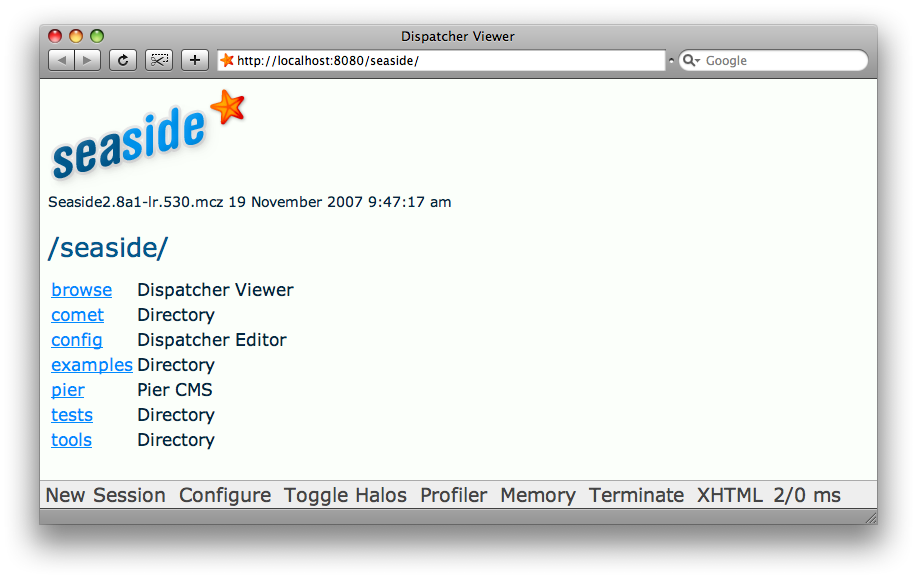
\includegraphics[width=\textwidth]{seasideStartup}
\caption{Seasideの初期画面
}
\figlabel{seasideStartup}
\end{center}
\end{figure}

\dothis{Seasideを開始してWebブラウザのURLを \url{http://localhost:8080/seaside/}にします。}

\noindent
\figref{seasideStartup}のようなページが表示されます。

\noindent
\dothis{\lct{examples{\go}counter}ページをクリックしてください。 (\figref{counter})}


\begin{figure}[htb]
\begin{center}
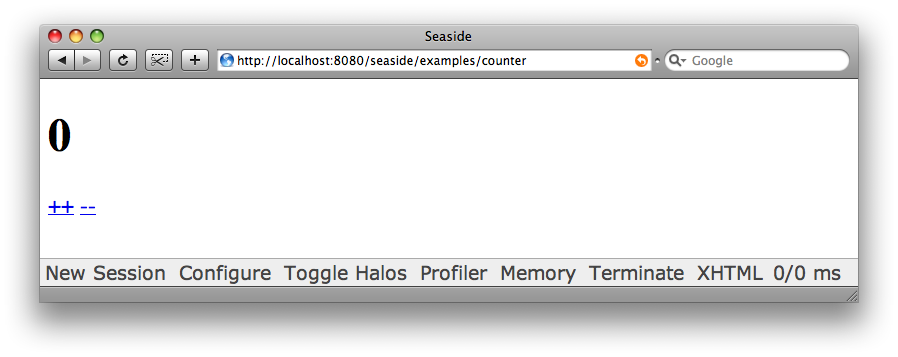
\includegraphics[width=0.8\textwidth]{counter}
\caption{カウンターのアプリケーション}
\figlabel{counter}
\end{center}
\end{figure}

\noindent
これはSeasideアプリケーションのサンプルです。\link{++}や \link{--\,--}のリンクをクリックするとカウンターの値を変えることができます。

\noindent
\dothis{リンクをクリックして値を変えてみましょう。Webブラウザの「戻る」ボタンで前の状態に戻ってから\link{++}のリンクを再びクリックしてみてください。
カウンターは、表示されていた値から増えています。決して「戻る」ボタンを押し始めたときの値からではないのです。}

今度は図\figref{seasideStartup}の\subind{Seaside}{toolbar}の初期画面の下のほうにあるツールバーに注目してみてください。
Seasideは「セッション」の概念をサポートしており、各アプリケーションはユーザごとに状態を管理できるようになっています。
\button{New Session} を押すと、アプリケーションの新たなセッションが始まります。
\button{Configure} ではアプリケーションの各種設定をWebブラウザ経由で行うことができます。

(\button{Configure}の画面を閉じるには、右上の \link{x} リンクをクリックします)。
\button{Toggle Halos} を押すと、Seasideで動作しているアプリケーションの状態が調べられます。
\button{Profiler} と \button{Memory} ボタンはアプリケーション実行時のパフォーマンスに関する詳細な情報を見るためのものです。

\button{XHTML} は生成されたWebページのXHTMLをバリデートするときに使います。対象とするページが外部からアクセス可能になっていないとこの機能は動作しません。W3Cのバリデータを使っているからです。
\index{Seaside!halos}

Seasideのアプリケーションは付け外し可能な「コンポーネント」からできています。フレームワークが提供する\ct{WAComponent}を継承したクラスのインスタンスであるということを除けば、コンポーネントは通常のSmalltalkのオブジェクトです。\pharo のイメージからコンポーネントやクラスを探索できますし、Webブラウザからハローを通じて直接たどっていくこともできます。

\begin{figure}[ht]
\begin{center}
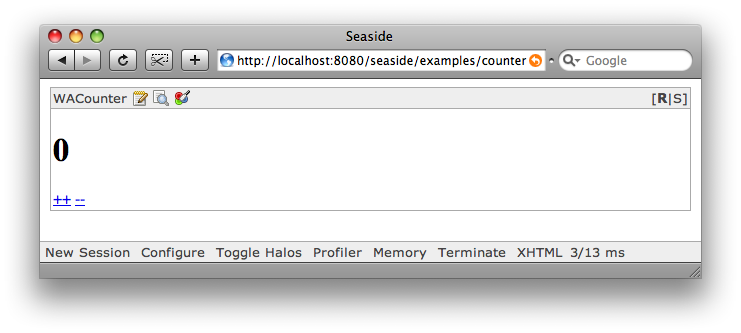
\includegraphics[width=\textwidth]{counterHalos}
\caption{ハロー}
\figlabel{counterHalos}
\end{center}
\end{figure}

\dothis{\button{Toggle Halos}を押してみましょう。\figref{counterHalos}のような画面になるはずです。
左上に\ct{WACounter}と表示されていますが、これは現在のページの構成要素となっているコンポーネントのクラス名を表しています。 
隣には3つのボタンアイコンがあります。
最初の鉛筆のアイコンは、このコンポーネントのクラスブラウザを開くためのものです。2番目の虫眼鏡アイコンでは、現在アクティブになっている\ct{WACounter}のインスタンスのインスペクタを開くことができます。
3番目の色のついた丸のボタンを押すと、コンポーネントについての\ind{CSS} スタイルシートエディタが表示されます。
右上には\link{R} と \link{S}のリンクがあります。それぞれクリックするとコンポーネントが通常表示とソース表示とに切り替わります。
こうしたリンクをすべて試してみましょう。
ソースビューの表示のときにも、\link{++} や \link{{-}{-}}は有効になっています。フォーマットもされているため、Webブラウザでソース表示をしたときよりも見やすいかもしれません。}

Seasideのクラスブラウザやオブジェクト・インスペクタは、サーバが別のマシンで動作していて、画面がなかったり、リモートの環境だったりするときには非常に便利です。
とはいえ、最初にSeasideのアプリケーションを開発するときには、ローカルでサーバを動かすと思います。その場合は\pharo のイメージが提供する普段の開発ツールのほうが使いやすいでしょう。

\begin{figure}[ht]
\begin{center}
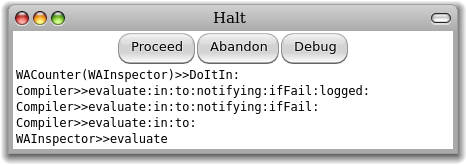
\includegraphics[width=0.7\textwidth]{haltingCounter}
\caption{カウンターアプリケーションをhaltさせる}
\figlabel{haltingCounter}
\end{center}
\end{figure}

%\dothis{Using the object inspector link in the web browser, open an inspector on the underlying Smalltalk counter object and evaluate \ct{self halt}}.
\dothis{Webブラウザのオブジェクト・インスペクタのリンクを使い、カウンターのインスペクタを開けてみて、 \ct{self halt}を実行してみましょう。
Webページはロード中の状態になります。Seasideのイメージのほうに移ってみてください。ノーティファイアが上がっていて (\figref{haltingCounter})、  \ct{WACounter} のオブジェクトが \ct{halt} の実行で止まっていることが確認できます。
さらにデバッガを開いて \button{Proceed} を押してみましょう。Webブラウザに戻るとカウンターは再び動作しています。}

Seasideのコンポーネントは、異なるコンテキストで何度も初期化できます。

\begin{figure}[ht]
\begin{center}
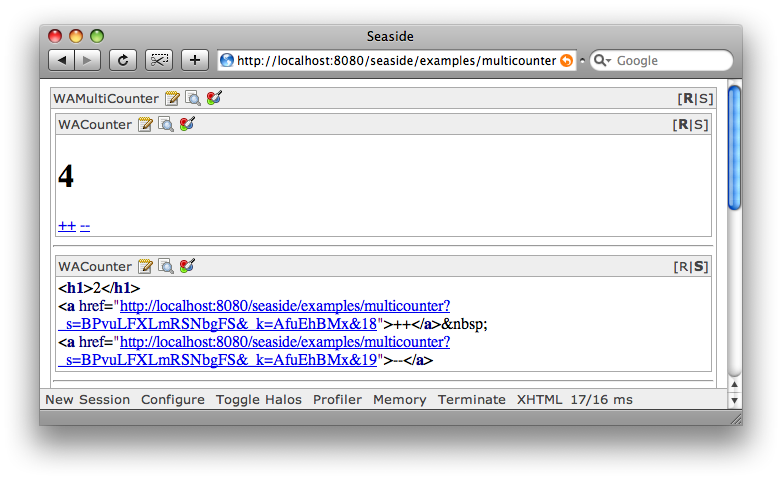
\includegraphics[width=\textwidth]{multiCounterHalos}
\caption{独立したサブコンポーネント}
\figlabel{multiCounterHalos}
\end{center}
\end{figure}

%\dothis{Point your web browser to \url{http://localhost:8080/seaside/examples/multicounter}}.
\dothis{WebブラウザのURLを\url{http://localhost:8080/seaside/examples/multicounter}に指定してみてください。
いくつもの独立したカウンターからなるアプリケーションが立ち上がります。
カウンターをいくつか選んで値を変えてみましょう。「戻る」ボタンを押しても問題なく動作します。
ハローを表示してみると、入れ子になったコンポーネント群からアプリケーションができていることがわかります。クラスブラウザを使って、 \ct{WAMultiCounter}の実装がどうなっているか見てみましょう。
クラスメソッドが3つ(\ct{canBeRoot}、 \ct{description}、 \ct{initialize})、インスタンスメソッドも3つ(\ct{children}、 \ct{initialize}、 \ct{renderContentOn:})定義されていることがわかります。
マルチカウンターのアプリケーションも、単なるコンポーネントです。クラスメソッドの\ct{canBeRoot}で \ct{true}を返し、コンポーネント階層のルートになるための宣言を行っているのです。}
\index{Seaside!multi-counter}

SeasideのWebインターフェースを使うと、アプリケーション(\ie ルートになるコンポーネント)を設定したり、コピーしたり、登録解除したりできます。設定を少しいじってみましょう。

\dothis{Webブラウザで\url{http://localhost:8080/seaside/config}を開きます。ユーザIDとパスワードを入れて、ログインしてください。(デフォルトでは\ct{admin} / \ct{seaside} となっています)。
``examples''の隣にある \link{Configure} をクリックします。 ``Add entry point''のところで、 ``counter2''と名前を入れ、タイプは \emph{Application} のまま \button{Add}ボタンをクリックします( \figref{counter2}を参照)。
次の画面で、 \emph{Root Component} を \clsind{WACounter}にして、 \button{Save} を押し、 \button{Close}で閉じます。
これでカウンターの新しいアプリケーションが \url{http://localhost:8080/seaside/examples/counter2}で起動するようになりました。
同様に、この設定ツール画面を通じて、登録したアプリケーションの解除を行うこともできます。
}
\index{Seaside!configuration}


\begin{figure}[ht]
\begin{center}
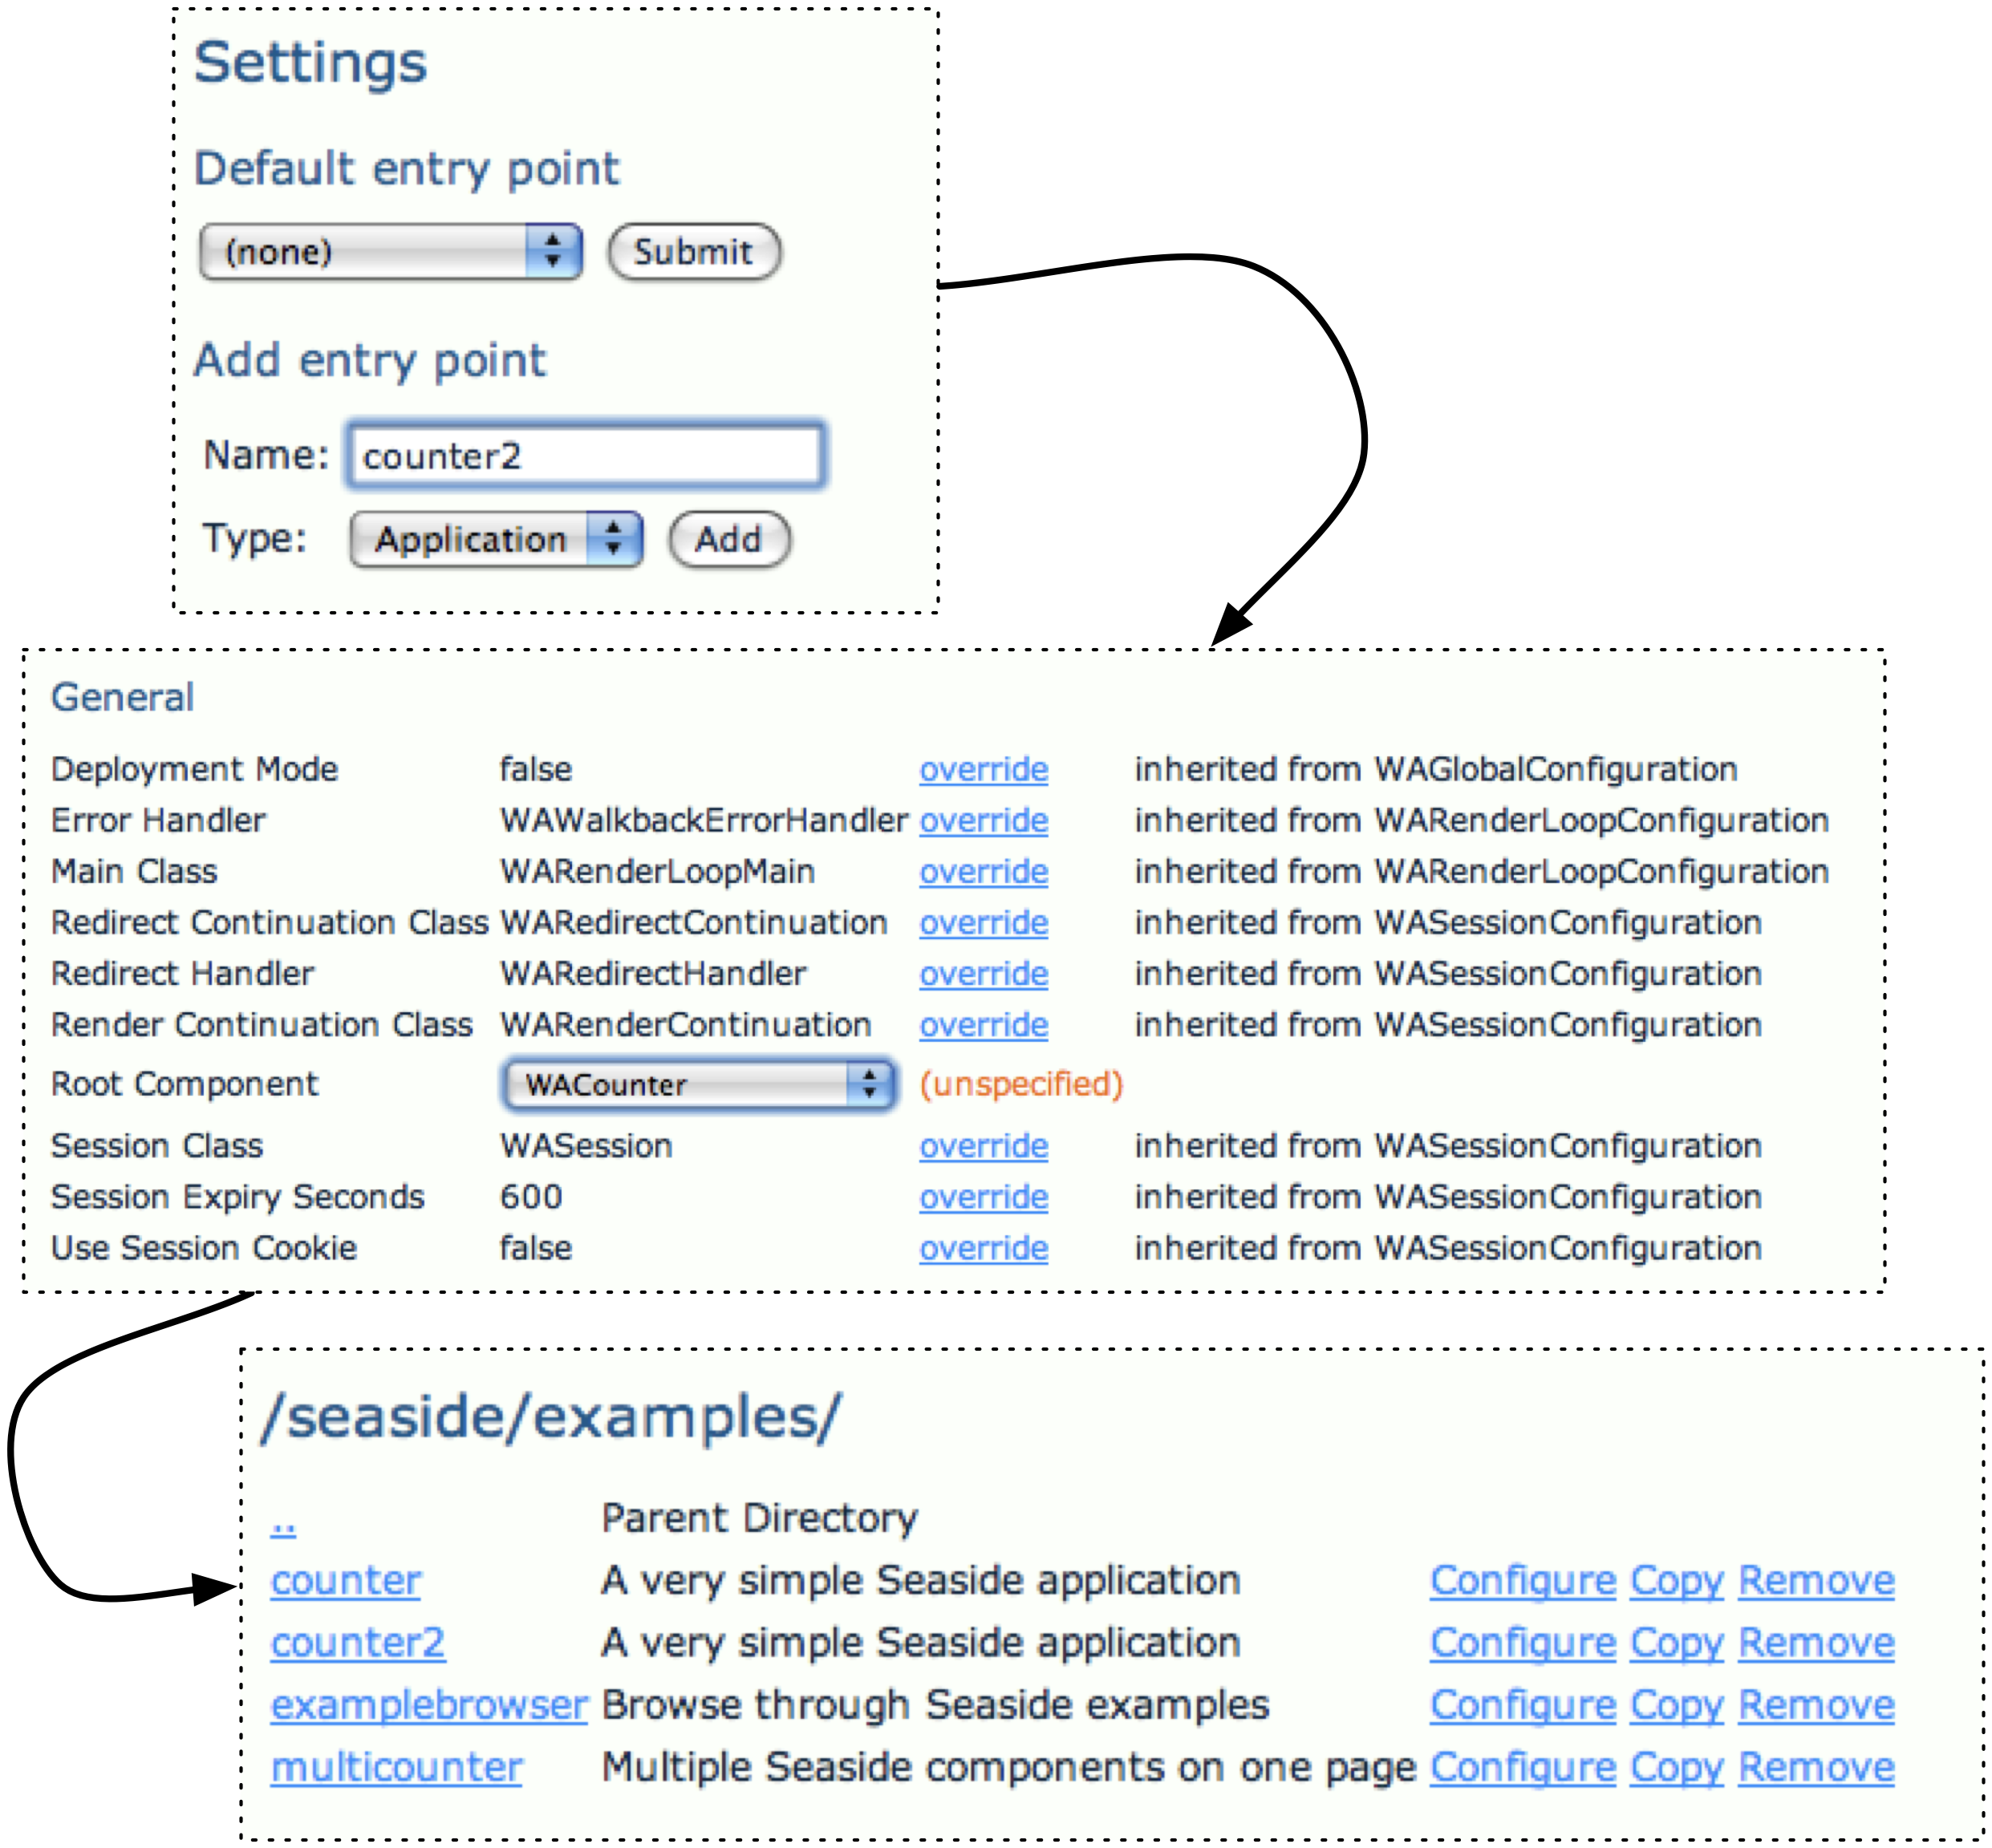
\includegraphics[width=\textwidth]{counter2}
\caption{新たなアプリケーションの設定}
\figlabel{counter2}
\end{center}
\end{figure}

Seasideは2つのモードで動作します。一つは今まで見てきた \emph{開発}モードです。 \emph{デプロイ} モードにすると、画面下のツールバーが非表示となります。
\index{Seaside!deployment mode}
\index{Seaside!development mode}

デプロイモードにするには、全体設定を行うツールのページからアプリケーションを選び、 \link{Configure} をクリックするか、ツールバーに表示されている \link{Configure} をクリックします。
% \ab{How?  I couldn't find this}
どちら場合も、デプロイモードのプルダウンボックスが表示されるので、\emph{true}に設定します。
この設定は新たなセッションを開始したタイミングで有効になります。
Seaside全体でモードを切り替えるには\clsind{WAGlobalConfiguration} \lct{setDeploymentMode}や、\ct{WAGlobalConfiguration setDevelopmentMode}を実行します。
\index{Seaside!deployment mode}
\index{Seaside!development mode}

設定ツール自体もSeasideのアプリケーションです。そのため同じようにWebブラウザから各種の設定ができます。もしも誤って``config'' のアプリケーションを削除してしまった場合は、
\clsind{WADispatcherEditor} \ct{initialize} とすると元に戻ります。

%=================================================================
\section{Seasideのコンポーネント}
\seclabel{components}

%\ab{This section was too long\,---\,18 pages.  It also contained several self-references (``see section 1.3''). So I broke into smaller sections, by promoting some of the subsections and subsubsections.}

前の節で示したように、Seasideのアプリケーションは\emph{\subind{Seaside}{コンポーネント}}から成り立っています。
\emph{Hello World}のコンポーネントを作成し、Seasideの仕組みをさらに詳しく見てみましょう。
コンポーネントを定義するには \clsind{WAComponent}を直接あるいは間接的に継承するようにします(\figref{WACounter})。

\dothis{ \ct{WAComponent}を継承した \ct{WAHelloWorld}クラスを定義してみましょう。}

コンポーネントでは自身の表示の仕方を定める必要があります。
このためには\mthind{WAPresenter}{renderContentOn:}をオーバーライドします。引数として XHTMLの生成方法を知っている\clsind{WAHtmlCanvas}が渡ってくるようになっています。
\index{Seaside!rendering}

\dothis{ \prot{rendering}プロトコルに以下のようにメソッドを定義してみましょう。}
\needlines{2}
\begin{code}{}
WAHelloWorld>>>renderContentOn: html
	html text: 'hello world'
\end{code}

\noindent
次に Seasideに対して、コンポーネントがスタンドアロンのアプリケーションであるという宣言を行います。

\dothis{\ct{WAHelloWorld} のクラス側に以下のメソッドを定義しましょう。}

\begin{code}{}
WAHelloWorld class>>>canBeRoot
	^ true
\end{code}

\noindent
これでほとんどできあがりです。

\dothis{Webブラウザで \url{http://localhost:8080/seaside/config}を開き、 ``hello''のエントリポイントを追加し、ルートのコンポーネントを \ct{WAHelloWorld}に設定します。
そしてURLを\url{http://localhost:8080/seaside/hello} に変えると、 \figref{WAHelloWorld}}のように表示されます!

\begin{figure}[htb]
\begin{center}
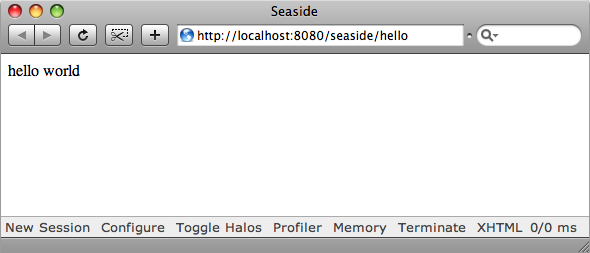
\includegraphics[width=\textwidth]{WAHelloWorld}
\caption{Seasideの``Hello World''}
\figlabel{WAHelloWorld}
\end{center}
\end{figure}

%-----------------------------------------------------------------
\subsection{状態のバックトラックと``Counter''アプリケーション}
%{Simple and nested components}

``hello world''に比べて、「カウンター」のアプリケーションは、ほんの少しだけ難しいものになっています。
\seclabel{backtracking}

\begin{figure}[ht]
\begin{center}
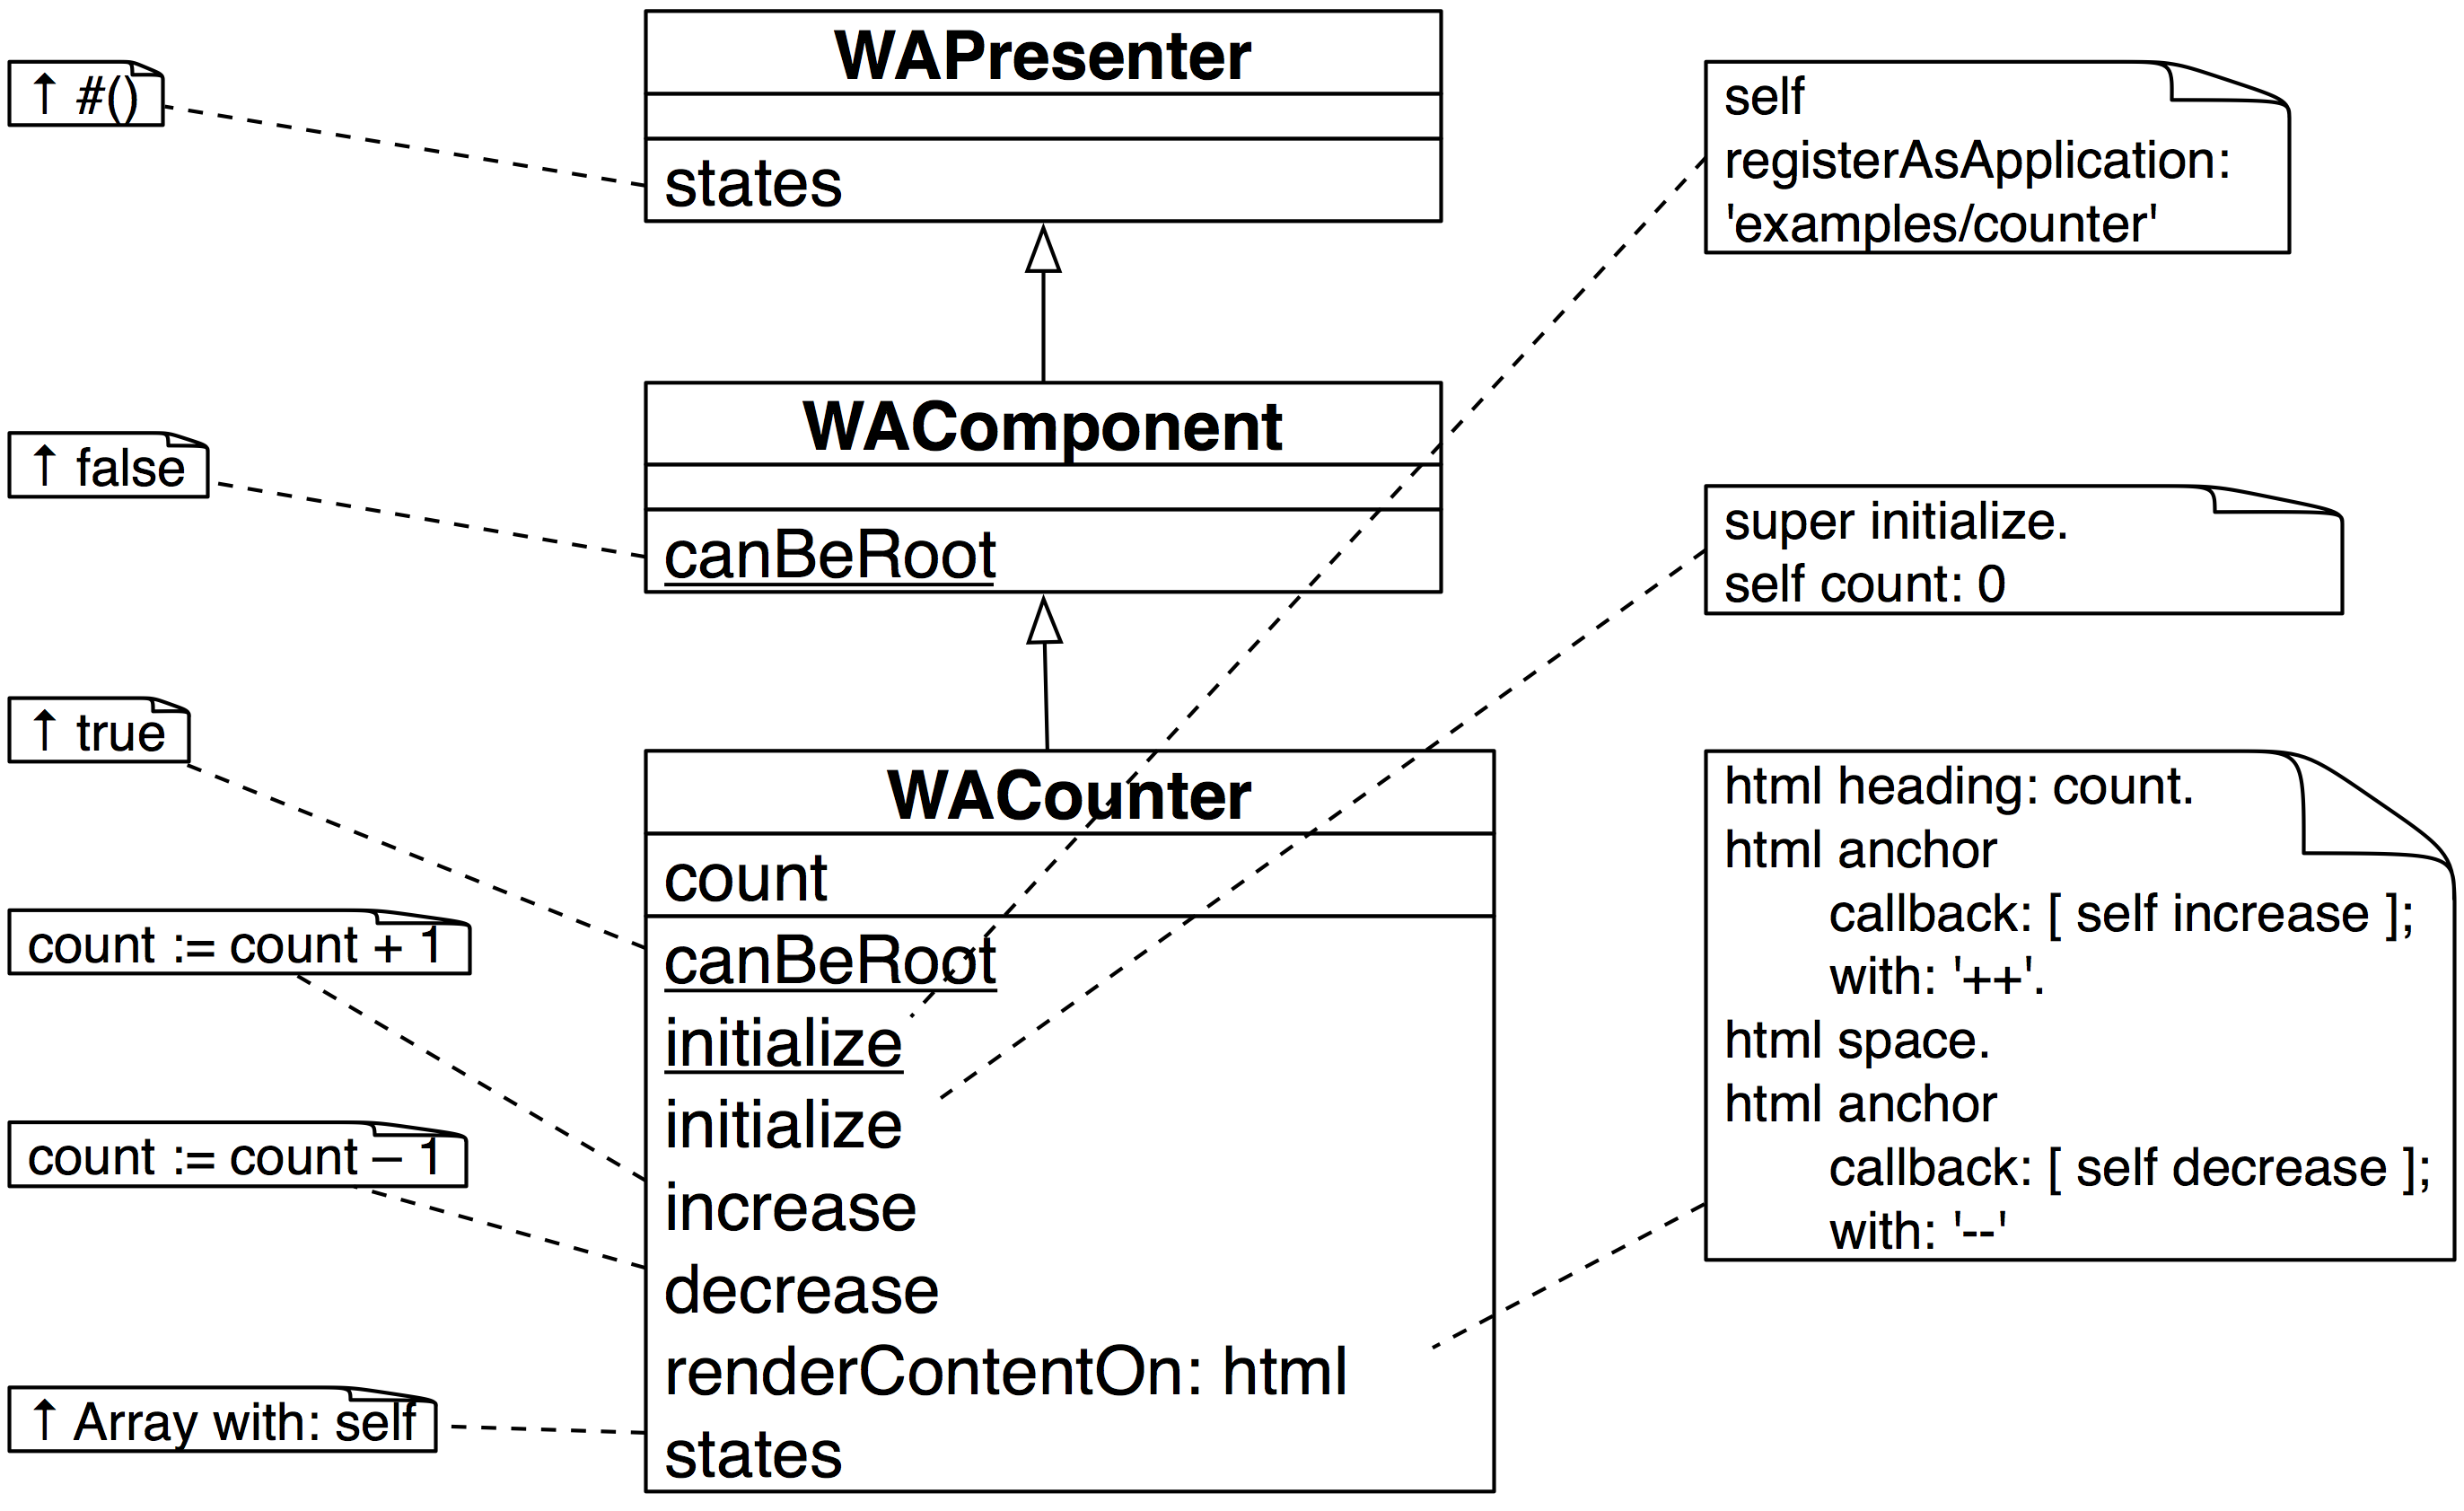
\includegraphics[width=\textwidth]{WACounter}
\caption{\emph{counter}アプリケーションは\ct{WACounter}クラスにより実装されています。  アンダーラインの引いてあるメソッドはクラスメソッドです。}
\figlabel{WACounter}
\end{center}
\end{figure}

 \clsind{WACounter} はスタンドアロンのアプリケーションなので \ct{WACounter class} では  \mthind{WAComponent class}{canBeRoot} を実装して、\ct{true} を返す必要があります。
 アプリケーションとしての登録は、図 \figref{WACounter}にあるように、クラスメソッド \ct{initialize}の中で行っています。

\ct{WACounter} には \ct{increase} と \ct{decrease}メソッドがあります。それぞれWebページで \link{++} 、 \link{--\,--} のリンクをクリックしたときに呼び出されます。カウンターの値を保持するため、インスタンス変数としては \ct{count}が定義してあります。
「戻る」ボタンを押してもカウンターの値がブラウザの値とずれないようにするには、\ct{WACounter} の状態をバックトラックするようにしなければなりません。
Seasideは、バックトラックのためのメカニズムを最初から持っていますが、アプリケーションのどの部分をバックトラックさせるかは開発者が指定する必要があります。

インスタンスメソッドの\ct{states}を実装すると、どの部分をバックトラック対象とするかを定めることができます。
% \ab{note that xspace messes up again, by inserting a space at the start of this line}
\ct{states} では対象とすべきオブジェクト群を配列の形で返すようにします。カウンターアプリケーションの場合、 \ct{Array with: self}としています。こうすると \ct{WACounter} のオブジェクト自身がSeasideにバックトラック対象として登録されることになります。

\paragraph{\emph{注意}}
バックトラック対象のオブジェクトの宣言ではちょっとした注意点があります。
Seasideは配列内のオブジェクトの\emph{copy}を取ることで、過去の状態を保持します。

実際の処理は \clsind{WASnapshot} によって行われます。 \ct{WASnapshot}は \clsind{IdentityDictionary} のサブクラスで、キーとしてバックトラック対象のオブジェクト群、値としてシャローコピーされたオブジェクト群を持っています。
特定のスナップショットに状態を戻す必要があるときには、シャローコピーされた情報を使って、オブジェクトの変数の値を上書きします。
先ほどの\ct{WACounter}の場合、バックトラックの対象は、インスタンス変数\ct{count} の数字だけで良いのではと思うかもしれません。しかし、  \ct{states} メソッドでr\ct{Array with: count} のように書いてもうまく動作しません。
これは\ct{count}の中身が整数で、整数は不変のオブジェクトだからです。
 \ct{increase} や \ct{decrease} メソッドでは、オブジェクトのそのものが \ct{0}から \ct{1} になったり、 \ct{3}から \ct{2}になっているわけではありません。
 \ct{count} 変数の中身が代入されて別の整数になっているのです。整数が増えたり減ったりするたびに、 \ct{count} が指すオブジェクトは 別のものに\emph{成り代わって}います。このため、 \ct{WACounter>>>states}では\ct{Array with: self}と書く必要があるのです。 \mbox{\ct{WACounter}} が以前の状態に戻るときには、各インスタンス変数の値がコピーされた\mbox{\ct{WACounter}}から復元されます。これで \ct{count} の値は正しく戻ることになります。
\index{Seaside!backtracking state}
\index{WAPresenter!states@\ct{states}}

\section{XHTMLのレンダリング}

Webアプリケーションでは、Webページを動的に生成して表示(レンダリング)を行います。 \secref{components}の節で述べたように、Seasideのコンポーネントは、それぞれが自身をレンダリングするようになっています。
仕組みを知るために、カウンターのコンポーネントがどのようにレンダリングを行っているか、見ていきましょう。

\subsection{カウンターのレンダリング}

カウンターのレンダリングは比較的単純です。 \figref{WACounter}のコードを見てください。
カウンターの現在の値がXHMLTの見出しとして表示されます。値の増減の操作はアンカー(リンク)として実装され、コールバックがブロックの形で仕掛けられています。アンカーをクリックすると \ct{increase} や \ct{decrease}がカウンターオブジェクトに対して送られるようになっています。

レンダリングで送るメッセージ群についてはすぐ後で詳しく解説しますが、その前に\subind{Seaside}{マルチカウンター}のほうもどうなっているか見てみましょう。

\subsection{CounterからMultiCounterへ}

まず \figref{WAMultiCounter} で示すように、\ct{WAMultiCounter}もスタンドアロンのアプリケーションなので、 \mthind{WAComponent class}{canBeRoot}を実装して \ct{true}を返すようにしています。

マルチカウンターのコンポーネントは、サブコンポーネントを含んだ \emph{コンポジット} となっています。そのため \ct{children} メソッドを実装して、中に含まれるコンポーネント群を配列の形で返しています。

レンダリングでは、サブコンポーネント群を、水平線で区切りを入れて表示するように書いています。
そのほか初期化を行うためのインスタンスメソッド、クラスメソッドがありますが、基本的にはこれだけで良いのです!

\begin{figure}[bht]
\begin{center}
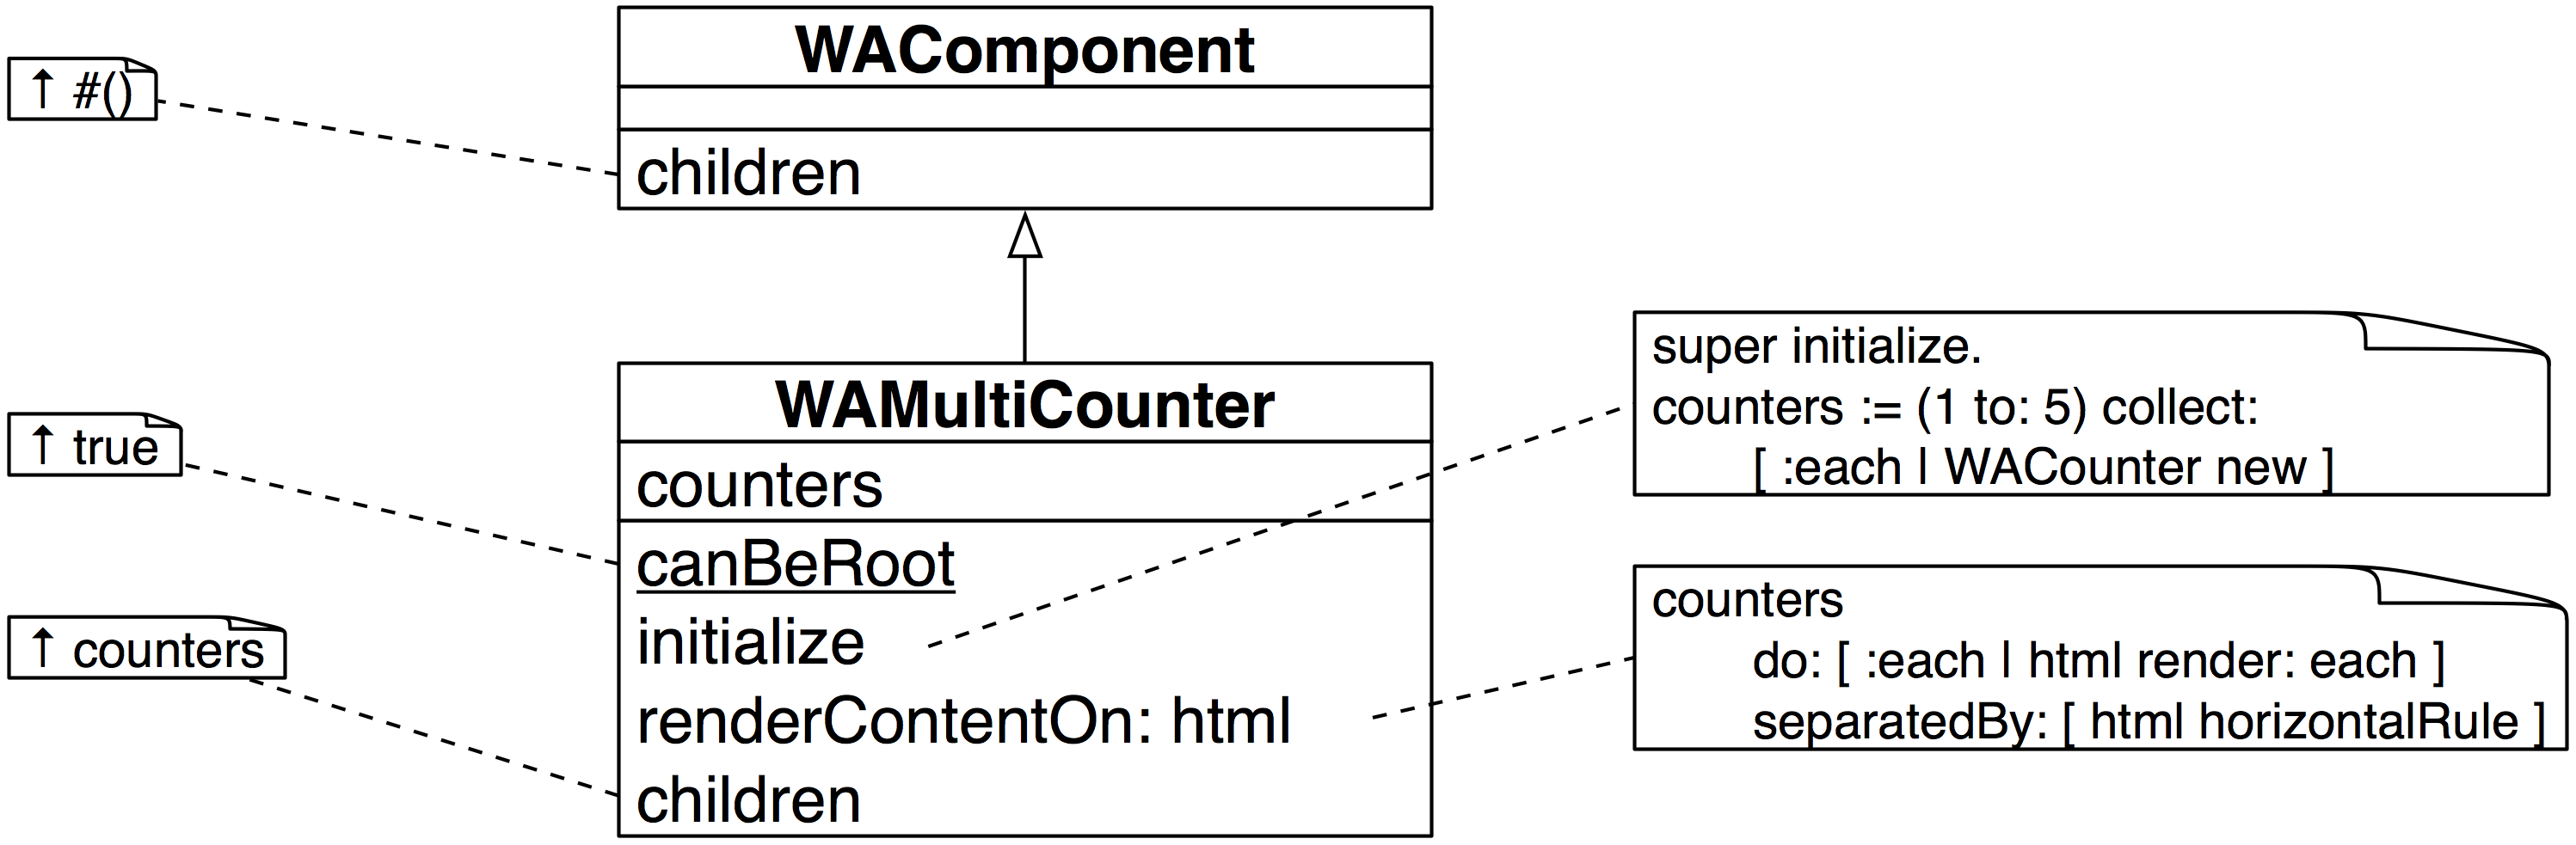
\includegraphics[width=\textwidth]{WAMultiCounter}
\caption{WAMultiCounter}
\figlabel{WAMultiCounter}
\end{center}
\end{figure}

%-----------------------------------------------------------------
\subsection{レンダリングの詳細}

今までの例で見てきたように、SeasideではWebページの生成にテンプレートを使いません。Smalltalkのメッセージ送信で生成するのです。
Seasideのコンポーネントは  \mthind{WAPresenter}{renderContentOn:}をオーバーライドする決まりになっています。このメソッドはコンポーネントのレンダリングのときにフレームワークの側から呼び出されます。
\ct{renderContentOn:} は、引数を一つ取りますが、 \seeindex{canvas}{htmlキャンバス} \emphind{htmlキャンバス}オブジェクトが渡ってくるようになっています。これを使ってコンポーネントはレンダリングを行います。慣習によりキャンバスは \ct{html} という名前になっています。htmlキャンバスはMorphicや別のGUIフレームワークでのキャンバスに似たものです。デバイス固有となる描画処理の詳細を、隠す役割を持っています。

基本的なレンダリングメッセージをいくつか挙げてみます。
\begin{code}{}
html text: 'hello world'.  "テキストを表示"
html html: '&ndash;'.     "XHTMLの直接指定"
html render: 1.              "オブジェクトのレンダリング"
\end{code}

\lct{任意のオブジェクト}を表示するには \ct{render: anObject} を使うことができます。通常はサブコンポーネントの表示で使われます。引数となった \lct{anObject}には \ct{renderContentOn:}のメッセージが内部的に送られます。
これはマルチカウンターの例で使いました ( \figref{WAMultiCounter}を参照)。

\subsection{ブラシの利用}
\seclabel{brushes}

キャンバス上で描画を行うために、たくさんの \emphind{ブラシ} を使うことができます。
XHTMLの各要素(段落、テーブル、リストなど)に対応したブラシがあります。
ブラシやそれに関連する便利メソッドを知るには、\clsind{WACanvas} とそのサブクラスをブラウズすると良いでしょう。
 \ct{renderContentOn:} の引数は、\clsind{WACanvas}を継承した \clsind{WARenderCanvas}のインスタンスになっています。

すでにカウンターとマルチカウンターの例で、以下のブラシを使いました。
\needlines{2}
\begin{code}{}
html horizontalRule.
\end{code}

\begin{figure}[ht]
\begin{center}
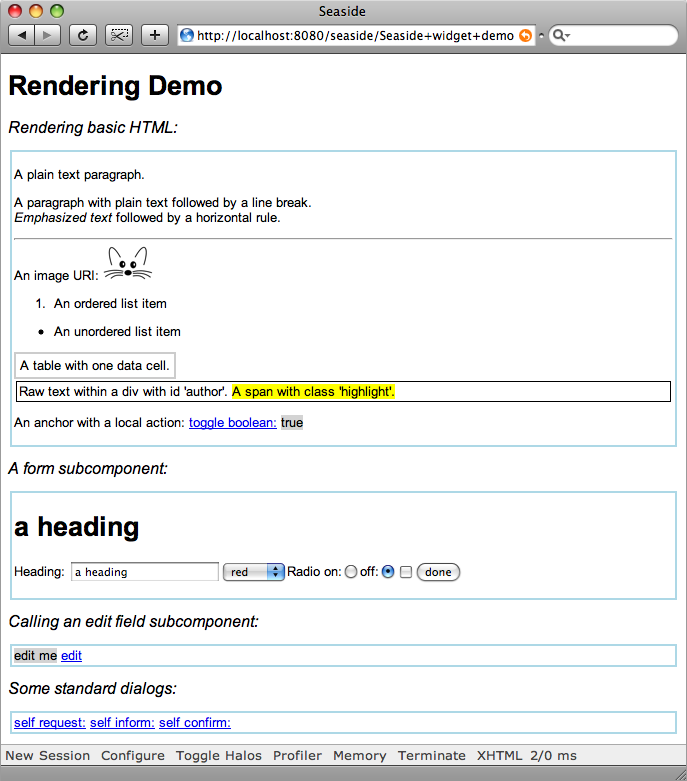
\includegraphics[width=\textwidth]{RenderingDemo}
\caption{レンダリングのデモ}
\figlabel{RenderingDemo}
\end{center}
\end{figure}

図 \figref{RenderingDemo}は、Seasideが提供する基本的なブラシをいろいろと使ってみた例です。 \footnote{
 \mthref{renderdemo}のソースコードは  \url{http://www.squeaksource.com/PharoByExample}プロジェクトの\ct{PBE-SeasideDemo}パッケージ内にあります。} \ct{SeasideDemo} のルートコンポーネントは単にサブコンポーネントの表示を行うだけです。サブコンポーネントは \mthref{renderdemo}を読むとわかりますが、\ct{SeasideHtmlDemo}、 \ct{SeasideFormDemo}、\ct{SeasideEditCallDemo} 、\ct{SeasideDialogDemo}となっています。
 
\needspace{7ex}
\begin{method}[renderdemo]{\lct{SeasideDemo>>renderContentOn:}}
SeasideDemo>>>renderContentOn: html
	html heading: 'Rendering Demo'.
	html heading
		level: 2;
		with: 'Rendering basic HTML: '.
	html div
		class: 'subcomponent';
		with: htmlDemo.
	"render the remaining components ..."
\end{method}

\noindent
コンポーネントはサブコンポーネントを返すというのを覚えているでしょうか。Seasideではレンダリングのたびにサブコンポーネントを再利用します。
\begin{code}{}
SeasideDemo>>>children
	^ { htmlDemo . formDemo . editDemo . dialogDemo }
\end{code}

上記のコードでは \ct{heading} ブラシの使い方が少し違っていることに注意してください。\ct{heading:}は、生成とともに、テキストをメッセージの引数でセットする書き方になっています。次に出てくるのは、\ct{heading}メッセージを送りブラシを生成してから、さまざまなプロパティをカスケードでセットしていくというものです。ブラシはたいていこの2種類の書き方ができるようになっています。

\important{もしも \ind{カスケード}を使って、ブラシに \mthind{WABrush}{with:}を送るなら、 \ct{with:} は必ず\emph{最後に}書く必要があります  message.
\ct{with:} によってブラシのレンダリングが始まるからです。}

\mthref{renderdemo}のメソッドでは、最初の見出しはデフォルトでレベルになります。次の見出しはレベル2を明示的に指定しています。
 サブコンポーネントはXHTMLで\emph{div}の中に囲まれる形になります。divには ``subcomponent''という\ind{CSS}のクラスを付与しています(CSSの使い方については\secref{css}で解説します)。  \ct{with:} メッセージの引数は、文字列とは限りません。この例ではコンポーネントを渡しています。次の例でも出てきますが、レンダリングの操作を記述したブロックでも良いのです。

\ct{SeasideHtmlDemo}コンポーネントは 基本的なブラシをいろいろと使ったデモになっています。コードを見ればだいたい利用の仕方がわかるでしょう。

\begin{code}{}
SeasideHtmlDemo>>>renderContentOn: html 
	self renderParagraphsOn: html.
	self renderListsAndTablesOn: html.
	self renderDivsAndSpansOn: html.
	self renderLinkWithCallbackOn: html
\end{code}

上のように、レンダリングのメソッドが長くなった場合には細かいメソッド群に分割することがよく行われます。

\important{一つのメソッド内に長々とレンダリング処理を書くやり方はお勧めできません。\ct{render*On:}という形でヘルパーメソッドとして分割しましょう。そうしたメソッド群は\prot{rendering} メソッドカテゴリーに置いておくようにします。また、 コンポーネントに\ct{renderContentOn:}を直接送ってはいけません。代わりに\ct{render:}を送るようにしてください。}

さらにコードを見ていきます。

最初の\ct{SeasideHtmlDemo>>>renderParagraphsOn:}ヘルパーメソッドは、XHTMLの段落、通常のテキスト、強調表示されたテキスト、画像の表示の例になっています。

Seasideでは、単純な要素なら単に文字列を指定するだけでレンダリングできますし、複雑なものであればブロックを使います。レンダリングのコードを書くときの指針として覚えておくと良いでしょう。

\begin{code}{}
SeasideHtmlDemo>>>renderParagraphsOn: html 
	html paragraph: 'A plain text paragraph.'.
	html paragraph: [
		html
			text: 'A paragraph with plain text followed by a line break. ';
			break;
			emphasis: 'Emphasized text ';
			text: 'followed by a horizontal rule.';
			horizontalRule;
			text: 'An image URI: '.
		html image
			url: self squeakImageUrl;
			width: '50']
\end{code}

次のヘルパーメソッド\ct{SeasideHtmlDemo>>>renderListsAndTablesOn:}は、リストとテーブルの表示例になっています。 テーブルではネストしたブロックを使い、列と列内のセルを表示します。

\begin{code}{}
SeasideHtmlDemo>>>renderListsAndTablesOn: html 
	html orderedList: [
		html listItem: 'An ordered list item'].
	html unorderedList: [
		html listItem: 'An unordered list item'].
	html table: [
		html tableRow: [
			html tableData: 'A table with one data cell.']]
\end{code}

次の例は、\emph{div}や \emph{span}の要素に、CSSの \emph{class} や \emph{id} 属性を指定するやり方を示しています。もちろん
 \ct{class:} や \ct{id:} といったメッセージは、\emph{div} \emph{span}以外のブラシにも送ることができます。
\ct{SeasideDemoWidget>>>style} のメソッドで、XHTMLの要素が実際にどのようなスタイルで表示されるかを定義しています(\secref{css}を参照)。

\begin{code}{}
SeasideHtmlDemo>>>renderDivsAndSpansOn: html 
	html div
		id: 'author';
		with: [
			html text: 'Raw text within a div with id ''author''. '.
			html span
				class: 'highlight';
				with: 'A span with class ''highlight''.']
\end{code}

最後に、リンクの簡単な例を見てみましょう。アンカー(リンク) にコールバックを設定しています。リンクをクリックするたびに、文字列が``true''と``false''に切り替わりますが、これはインスタンス変数の\ct{toggleValue}の値がコールバックの実行により変化するからです。

\needlines{3}
\begin{code}{}
SeasideHtmlDemo>>>renderLinkWithCallbackOn: html 
	html paragraph: [
		html text: 'An anchor with a local action: '.
		html span with: [
			html anchor
				callback: [toggleValue := toggleValue not];
				with: 'toggle boolean:'].
		html space.
		html span
			class: 'boolean';
			with: toggleValue ]
\end{code}

\important{アプリケーションの状態を変えるような処理は、コールバック内に書くようにします。
レンダリング中に、直接そのようなコードを書くべきではありません。}

%-----------------------------------------------------------------
\subsection{フォーム}

フォームも今までの例と同様のやり方で表示できます。
図\figref{RenderingDemo}の\ct{SeasideFormDemo} コンポーネントのコードを示します。
\index{Seaside!XHTML forms}

\begin{code}{}
SeasideFormDemo>>>renderContentOn: html
	| radioGroup |
	html heading: heading.
	html form: [
		html span: 'Heading: '.
		html textInput on: #heading of: self.
		html select
			list: self colors;
			on: #color of: self.
		radioGroup := html radioGroup.
		html text: 'Radio on:'.
		radioGroup radioButton
			selected: radioOn;
			callback: [radioOn := true].
		html text: 'off:'.
		radioGroup radioButton
			selected: radioOn not;
			callback: [radioOn := false].
		html checkbox on: #checked of: self.
		html submitButton
			text: 'done' ]
\end{code}{}

フォーム要素は複雑なので、ブロックを使ってレンダリングします。状態の変更に関わるコードはすべてコールバック内で書かれており、レンダリング部分には書かれないことに注意してください。

 \mthind{WAAnchorTag}{on:of:}については説明が必要でしょう。
上の例ではテキストフィールドに、自身のインスタンス変数\ct{heading}を対応させるために使われています。
アンカーやボタンもこのメッセージに答えられます。

最初の引数はインスタンス変数の名前です。2番目の引数は変数を保持するオブジェクトを指定します。
通常の名前付けルールで、インスタンス変数のアクセッサー (\ct{heading}) とミューテイター (\ct{heading:})がクラスに定義されていることが前提となっています。

上記のテキストフィールドの例では、デフォルト値の設定や、値を更新するためのコールバックを書く手間を省くのに役立っています。 \ct{on: #heading of: self}を使うことで \ct{heading} 変数の値はユーザの入力に応じて自動的に更新されます。

すぐ後にコンボボックスで\ct{color} 変数を指定した別の例があります。その次のチェックボックスの例では、 \ct{checked} 変数の値が更新されるようになっています。

Seasideの機能テストのコードを見ると、さらにさまざまなフォームの例が見つかります。
%2.8ベース。修正の必要あり(ume) 
% URL -> http://localhost:8080/tests/functional/WAInputPostFunctionalTest
% menu -> WAInputGetFunctionalTest, (WAInputPostFunctionalTest)
 \scat{Seaside-Tests-Functional}のクラスカテゴリを見てみましょう。また、Webブラウザで\url{http://localhost:8080/seaside/tests/alltests}のURLを指定し、
\menu{WAInputTest} を選んで \button{Restart} ボタンを押すと、フォームのほとんどの機能を知ることができます。

Webブラウザの\button{Toggle Halos}ボタンを押せば、対応するソースコードにすぐにアクセスできるというSeasideの機能を、ここで活用してください。

%-----------------------------------------------------------------
\section{CSS: カスケーディング・スタイル・シート}
\seclabel{css}

%\ab{I think that it just needs a few paragraphs telling the reader the key ideas behind CSS, and the new terminology that the CSS folks introduce, before going in to the details of how you define their "thingies".  Now I have forgotten what they call their "thingies" --- I know that there are effectively paragraph styles (divs) and character styles (spans), but I've forgotten what they call them.  So, I think that the text needs to tell the reader, for each thingie, (1) the CSS concept behind the thingie, (2) what it looks like in a CSS style sheet , (3) what it looks like in html, and (4) how to do it in Seaside.   Maybe (3) can be omitted, because it's not needed to use Seaside.}
% \on{I think we do most of that already.}

\ind{CSS}(カスケーディング・スタイル・シート) \footnote{\url{http://www.w3.org/Style/CSS/}}は、Webアプリケーションで、内容と見栄えを分離する標準的な方法になっています。Seasideでは、レンダリングのコードが見栄えを意識して煩雑になるのを、CSSの技術を使って防いでいます。

 \ct{style}というメソッドをコンポーネントに定義することで、使用するスタイルシートを決めることができます。メソッドの中身は、コンポーネントが使うスタイルについて定めた単なるCSSの文字列です。

Webページに配置されるコンポーネントのスタイルシートは結合されて一つになりますが、コンポーネントは自身のスタイルを自ら定義できます。抽象クラスを定義して、アプリケーションで使う共通のスタイルをメソッドとして定義しておくのも良いでしょう。

とはいえデプロイ時には、外部ファイルとしてスタイルシートを用意することも広く行われます。こうするとコンポーネントの機能的な部分と、見栄えの分離がさらに進み、完全に分離されることになります。
( \clsind{WAFileLibrary}クラスを使うと、別途サーバを用意せずに、外部のファイルを利用可能です)。

CSSをよく知っているのでしたら、これで説明は終わりです。念のため、以後は簡単なCSSの紹介を書いておきます。

CSSを使うと、段落やテキストの表示属性を直接Webページに埋め込む代わりに、表示情報を分類分けして、別途スタイルシートに定義できます。段落に該当する要素が \emph{div}で、インラインのテキスト要素は \emph{span} と呼ばれます。
例えば自分で``highlight''といった形で、要素に名前をつけ、ハイライトされるテキストを定義することができます(例を参照のこと)。スタイルシートの中では、ハイライトがどのように表示されるべきかを記述します。

基本的に CSS は、XHTMLの要素をどのようなフォーマットで表示するかについてのルールを記述したものです。ルールは二つの部分から成り立っています。
 \emph{セレクター}と呼ばれる部分では、どの XHTML 要素にルールを適用するかを指定します。 \emph{宣言} の箇所では、要素に適用される属性の値を定めます。

\begin{figure}[tb]
\begin{code}{}
SeasideDemoWidget>>>style
	^ '
body {
	font: 10pt Arial, Helvetica, sans-serif, Times New Roman;
}
h2 {
	font-size: 12pt;
	font-weight: normal;
	font-style: italic;
}
table { border-collapse: collapse; }
td {
	border: 2px solid #CCCCCC;
	padding: 4px;
}
#author {
	border: 1px solid black;
	padding: 2px;
	margin: 2px;
}
.subcomponent {
	border: 2px solid lightblue;
	padding: 2px;
	margin: 2px;
}
.highlight { background-color: yellow; }
.boolean { background-color: lightgrey; }
.field { background-color: lightgrey; }
'
\end{code}
\caption{\lct{SeasideDemoWidget} 共通スタイルシート
\figlabel{democss}}
\end{figure}

\figref{democss} は、\figref{RenderingDemo}で使われているスタイルシートのメソッドを示したものです。
最初のルールは \ct{body}要素で使われるフォントを指定しています。さらに、見出しレベル2 (\ct{h2})、テーブル (\ct{table})、セル (\ct{td})についての定義が続きます。

残りのルールは、特定の``class'' や ``id''を持つ XHTML要素についてです。クラス属性のCSSのセレクターは``\ct{.}''でid 属性のセレクターは``\ct{#}''で始まります。
classと id の違いは、ページ内でid属性の要素は一つしか存在できませんが(\emph{IDのため})、クラス属性の要素は複数あっても良いということです。 \ct{highlight}はクラス属性なので、ページ内に何度出てきてもかまいません。id属性はページ内で \emph{唯一}の要素、例えばメニュー、更新日、作者の名前などで使われます。また、XHTMLの各要素には、複数のクラス属性が指定できます。その場合は指定された順番に沿って、表示の属性が適用されていきます。

% This style sheet expects at most one element to specify the \emph{author} of the web page.

セレクターは組み合わせることができます。 \ct{div.subcomponent} というセレクターは、divで、クラス属性が``subcomponent''の要素のみを選択することになります。

あまり必要になることはありませんが、ネストした要素を指定することも可能です。例えば ``\ct{p span}''は、段落内(p)のspanを選択します。div内のspanにマッチすることはありません。

CSSについては多くの本やWebページがあります。CSSでどれだけのことができるかを知るには、CSS Zen Garden\footnote{\url{http://www.csszengarden.com/}}のサイトを見てみると良いでしょう。CSSのスタイルシートを変えるだけで、同じ内容の文書をまったく異なる見栄えにできるということがわかります。

%-----------------------------------------------------------------
\section{制御フローの管理}

Seaside では、複雑なフローを持つWebアプリケーションを、非常に簡単に開発できるようになっています。二つの基本的な仕組みが提供されています。

\begin{enumerate}
  \item コンポーネントは、\ct{caller call: callee}のように書くことで、他のコンポーネントを\emph{呼び出す}ことができます。呼び出し側は一時的に表示されなくなり、呼ばれた側に制御が移ります。\ct{answer:}によって、制御を元に返すことができます。呼び出し側は通常 \ct{self}ですが、現在表示されているコンポーネントであればどれでもかまいません。

  \item 全体のワークフローは \emphsubind{Seaside}{タスク}の仕組みで定義できます。\clsind{WAComponent}でなく、\clsind{WATask}を継承することで、特別なコンポーネントになります。 \seclabel{task} タスクは内部にコンポーネントを持ちません。
   \ct{renderContentOn:}を実装する代わりに、 \ct{go} メソッドを定義し、コンポーネントを順番に \ct{call:}する形で全体の流れを書いていきます。
  
\end{enumerate}
\index{Seaside!control flow}

%-----------------------------------------------------------------
\subsection{call:とanswer:}

call:とanuswer:は単純なダイアログ形式のUIを実現するために使われます。

 \ct{call:} と \ct{answer:} を使った簡単な例は、図\figref{RenderingDemo}のレンダリングのデモに含まれています。
 \ct{SeasideEditCallDemo} のコンポーネントは、テキストフィールドと \emph{edit}リンクを表示しています。editのリンクにはコールバックが仕掛けられていて、\ct{SeasideEditAnswerDemo}のインスタンスを、テキストフィールドの値で初期化した上で呼び出すようになっています。コールバックではさらに、呼び出したコンポーネントから受け取った値を、テキストフィールドに反映させるようになっています。
 
(以下のコード例では目立たせるために \ct{call:} と \ct{answer:} のメッセージにアンダーラインを引いています)。

\begin{code}{}
SeasideEditCallDemo>>>renderContentOn: html 
	html span
		class: 'field';
		with: self text.
	html space.
	html anchor
		callback: [self text: (self !\underline{call:}! (SeasideEditAnswerDemo new text: self text))];
		with: 'edit'
\end{code}{}

次に表示すべきWebページ全体を意識する部分がまったくない、というところがエレガントです。実行すると \ct{SeasideEditCallDemo} コンポーネントが表示している部分が \ct{SeasideEditAnswerDemo} コンポーネントに置き換わり、ページ全体の表示が行われます。外側のコンポーネントや隣接するコンポーネントはそのままです。

\important{\mthind{WAComponent}{call:} や \mthind{WAComponent}{answer:} はレンダリングの中に直接記述してはいけません。\subind{Seaside}{コールバック}や、タスクの\mthind{WATask}{go}メソッドの中で書くようにします。}

\ct{SeasideEditAnswerDemo} コンポーネントも非常にシンプルです。テキストフィールドの初期値を表示し、送信ボタンのコールバックで、更新されたテキストフィールドの値を返すように書いてあるだけです。

\begin{code}{}
SeasideEditAnswerDemo>>>renderContentOn: html
	html form: [
		html textInput
			on: #text of: self.
		html submitButton
			callback: [ self !\underline{answer:}! self text ];
			text: 'ok'.
		]
\end{code}{}

わずかこれだけでページの遷移が実現できます。

Seaside は適切なコンポーネントに制御を移し、レンダリングを自動的に行ってくれます。Webブラウザの「戻る」ボタンも問題なく動作します。 (ただし副作用をロールバックできるようにするにはもう少しコードが必要になります)。

%-----------------------------------------------------------------
\subsection{便利なメソッド群}

call/answerを使ったやりとりには非常に良く出てくるパターンがあります。そのためSeasideは、\ct{SeasideEditAnswerDemo}のような些細なコンポーネントをわざわざ書かずにすむように、便利なメソッドを提供しています。便利メソッドによって生成されるダイアログを図で示しました(\figref{dialogs})。これらの便利メソッドの動作は \ct{SeasideDialogDemo>>>renderContentOn:}で確認できます。

\begin{figure}[b]
\begin{center}

\includegraphics[width=\textwidth]{dialogs}
\caption{標準ダイアログ}
\figlabel{dialogs}
\end{center}
\end{figure}

\mthind{WAComponent}{request:}では、編集可能なテキストフィールドつきのコンポーネントが開きます。ユーザが入力したテキストが呼び出し側に返るようになっています。ラベルやデフォルト値も指定できます。

\needlines{3}
\begin{code}{}
SeasideDialogDemo>>>renderContentOn: html
	html anchor
		callback: [ self request: 'edit this' label: 'done' default: 'some text' ];
		with: 'self request:'.
...
\end{code}

\mthind{WAComponent}{inform:} では、指定した文字列を表示するコンポーネントが開きます。``ok''ボタンを押すとコンポーネントが閉じ、制御が呼び出し側に戻ります。このコンポーネントは\ct{self}を返すだけです。

\begin{code}{}
...
	html space.
	html anchor
		callback: [ self inform: 'yesBANG' ];
		with: 'self inform:'.
...
\end{code}

\mthind{WAComponent}{confirm:} を使うと``Yes''/``No''の質問ダイアログとなり、ユーザはどちらかを選ぶことになります。真偽値を呼び出し側に返すので、それによって次の動作を決めることができます。

\begin{code}{}
...
	html space.
	html anchor
		callback: [
			(self confirm: 'Are you happy?')
				ifTrue: [ self inform: ':-)' ]
				ifFalse: [ self inform: ':-(' ]
			];
		with: 'self confirm:'.
\end{code}

\clsind{WAComponent}の\prot{convenience}プロトコルには、 \mthind{WAComponent}{chooseFrom:caption:}ような役に立つメソッドがさらに定義してあります。

%-----------------------------------------------------------------
\subsection{タスク}

 \clsind{WATask}を継承すると、\subind{Seaside}{タスク}を定義できます。タスクは自身ではレンダリングを行いません。単に制御フローに沿って他のコンポーネントをcall:していくだけです。 \mthind{WATask}{go}に、制御の流れを書いていきます。

\scat{Seaside-Tests-Functional}クラスカテゴリに定義されている\clsind{WAConvenienceTest} は、タスクの簡単な使用例になっています。動作を確認するには、Webブラウザで \url{http://localhost:8080/seaside/tests/alltests}のURLを開き、 \menu{WAConvenienceTest} を選択して \button{Restart}ボタンを押します。

%URLが古い。該当するクラスも3.0には存在しない。

\begin{code}{}
WAConvenienceTest>>>go
	[ self chooseCheese.
	  self confirmCheese ] whileFalse.
	self informCheese
\end{code}

このタスクでは3つのコンポーネントの呼び出しを順次行っています。まず\mthind{WAComponent}{chooseFrom: caption:}の便利メソッドで、\clsind{WAChoiceDialog}のダイアログが開きます。ここでユーザーは好きなチーズを選択します。

\begin{code}{}
WAConvenienceTest>>>chooseCheese
	cheese := self
		chooseFrom: #('Greyerzer' 'Tilsiter' 'Sbrinz')
		caption: 'What''s your favorite Cheese?'.
	cheese isNil ifTrue: [ self chooseCheese ]
\end{code}

% \alex{Is there a situation where cheese may be nil? Maybe if a browser authorizes an empty selection...}

次に \clsind{WAYesOrNoDialog} でユーザーの選択を確認します(ダイアログは\mthind{WAComponent}{confirm:}で生成されたものです)。

\begin{code}{}
WAConvenienceTest>>>confirmCheese
	^self confirm: 'Is ', cheese,  ' your favorite cheese?'
\end{code}

最後に便利メソッド \mthind{WAComponent}{inform:})によって、\clsind{WAFormDialog} が呼び出されます。

\begin{code}{}
WAConvenienceTest>>>informCheese
	self inform: 'Your favorite cheese is ', cheese, '.'
\end{code}

生成されるダイアログを図 \figref{chooseCheese}に示します。

\begin{figure}[ht]
\begin{center}
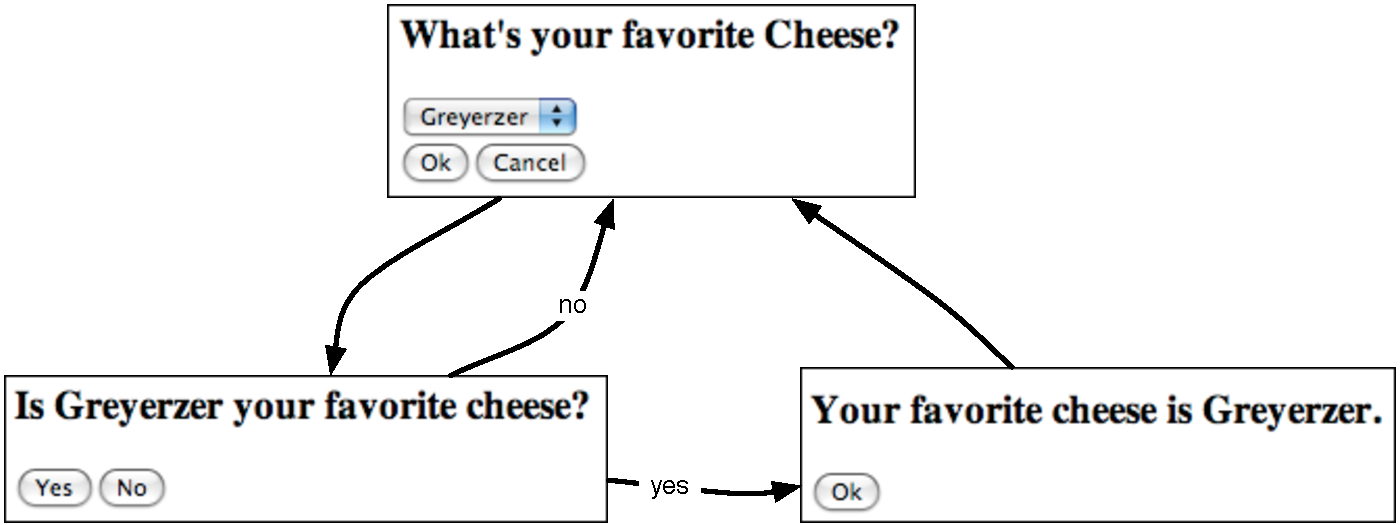
\includegraphics[width=\textwidth]{chooseCheese}
\caption{単純なタスクの例}
\figlabel{chooseCheese}
\end{center}
\end{figure}

%-----------------------------------------------------------------
\subsection{トランザクション}
% 3.0で未サポートとなった機能。訳す?

 \secref{backtracking} の節で、 Seasideではバックトラック対象となるオブジェクトを登録することで、コンポーネントの状態をWebページごとに記録できるという話をしました。コンポーネント側で必要なのは、 \ct{states} メソッドを定義し、バックトラック対象のオブジェクトを配列の形で返すことだけでした。

しかし時にはバックトラックをしたくないときもあります。ユーザーが行った操作を、意図せず取り消してしまうことを\emph{防ぎたい}ときがあるのです。これは「ショッピングカート問題」などと呼ばれます。ユーザーがショッピングカートの精算を済ませた後は、Webブラウザのボタンで戻って、カートに商品を追加できてしまってはまずいのです。

Seasideでは、一連の操作をひとまとめにしてタスク内で\emph{トランザクション}として定義することにより、この問題を解決します。トランザクション内ではバックトラックができますが、トランザクションが終了すると戻ることはできません。トランザクションを越えて戻ろうとしても、前のページは \emph{無効}になります。無効なページの表示時にSeasideが警告を出し、直近の有効なページへと自動的にリダイレクトします。

\begin{figure}[ht]
\begin{center}
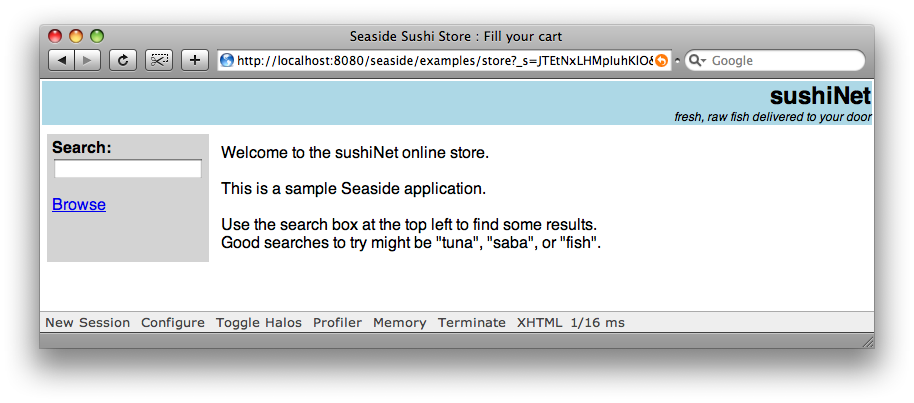
\includegraphics[width=\textwidth]{sushiStore}
\caption{寿司屋デモ}
\figlabel{sushiStore}
\end{center}
\end{figure}

\emphsubind{Seaside}{寿司屋デモ} は、Seasideの多くの特徴を示すサンプルアプリケーションです。もちろんトランザクションも使われています。
このサンプルはSeasideに含まれており、Webブラウザで\url{http://localhost:8080/seaside/examples/store}のURLを指定すると起動します。\footnote{もしも同梱されていない場合はSqueakSourceのページ(\url{http://www.squeaksource.com/SeasideExamples/})からロードできます。 }

寿司屋デモのワークフローは以下のようになっています。
\begin{enumerate}[itemsep=0pt]
  \item サイトを訪れる
  \item 寿司をブラウズ、または検索する
  \item ショッピングカートに寿司を追加する
  \item 注文を開始する
  \item カートの内容を確認する
  \item 届け先の住所を入力する
  \item 住所を確認する
  \item 支払い情報を入力する
  \item 寿司を待つ
\end{enumerate}

 \subind{Seaside}{ハロー}を表示してみると、トップレベルのコンポーネントは \clsind{WAStore}となっていることがわかります。自身はタイトルバーの表示を行っているだけで、\clsind{WAStoreTask}のインスタンスである \ct{task}にレンダリングを委譲しています。

\begin{code}{}
WAStore>>>renderContentOn: html
	"... render the title bar ..."
	html div id: 'body'; with: task
\end{code}

ワークフローの順番を定義しているのが\clsind{WAStoreTask}です。一度サブミットした情報を、ユーザーが戻って変更できないようにしていることが重要です。

\dothis{\,いくつか寿司を購入した後で、カートの中にさらに寿司を追加するため、Webブラウザの「戻る」ボタンを押してみましょう。``That page has expired.''と出て追加できません。}

Seasideでは、プログラマがワークフローの特定部分をトランザクションとして定義できるようになっています。トランザクションが終了すると、ユーザはそこに戻って操作をやり直すことはできません。
トランザクションを定義するには、\mthind{WAComponent}{isolate:}メッセージをタスクに送ります。引数で
トランザクション部分ブロックで指定します。寿司屋デモでは以下のようにしています。

\begin{code}{}
WAStoreTask>>>go
	| shipping billing creditCard |
	cart := WAStoreCart new.
	self isolate:
		[[self fillCart.
		self confirmContentsOfCart]
			whileFalse].

	self isolate:
		[shipping := self getShippingAddress.
		billing := (self useAsBillingAddress: shipping)
					ifFalse: [self getBillingAddress]
					ifTrue: [shipping].
		creditCard := self getPaymentInfo.
		self shipTo: shipping billTo: billing payWith: creditCard].

	self displayConfirmation.
\end{code}

2つのトランザクションが定義されています。最初のトランザクションは、カートに寿司を入れて内容を確認する部分です。( \ct{fillCart} 等のヘルパーメソッドは、内部でサブコンポーネントを生成したり呼び出したりしています)。

%原文ではセッションを開始しない限り、とあるが、どちらにせよ「戻る」ことはできない
一度カートの確認を終えてしまうと、戻ることはできません。2番目のトランザクションは、住所と支払い方法を入れる部分です。支払い方法を確定するまでは、このトランザクション内で戻ることもできます。
トランザクションを終えると、戻ろうとしても常に警告が出て失敗します。

トランザクションをネストすることもできます。 \clsind{WANestedTransaction}で簡単なデモを見ることができます。
% 3.0には同梱されていない
最初の \ct{isolate:}のブロック内に、さらに別の \ct{isolate:}ブロックが含まれています。

\begin{code}{}
WANestedTransaction>>>go
	self inform: 'Before parent txn'.
	self isolate:
			[self inform: 'Inside parent txn'.
			self isolate: [self inform: 'Inside child txn'].
			self inform: 'Outside child txn'].
	self inform: 'Outside parent txn'
\end{code}

\dothis{\url{http://localhost:8080/seaside/tests/alltests}を開いて \menu{WATransactionTest} のメニューを選び 、\button{Restart}ボタンを押してみましょう。親側と子側のトランザクション内で\button{OK}ボタンやブラウザの\button{戻る}ボタンを使い、行ったり来たりしてみましょう。トランザクション終了後は、戻って\button{OK}ボタンを押しても、エラーが出て終了後のページに必ずリダイレクトされます。}

%=================================================================
\section{サンプルアプリ作成によるチュートリアル}

% ON: Should take about two hours

ここではSeasideのアプリケーションを一から作成してみることにします。 \footnote{二、三時間はかかります。すべてのソースコードを見たい場合はSqueakSourceのプロジェクト \url{http://www.squeaksource.com/PharoByExample}から入手できます。 \scat{PBE-SeasideRPN}のパッケージを選んでロードします。クラス名を少し変えてあるので、すべて読み込んでも、本書に従ってアプリケーションを作っていくことができます。}
RPN (逆ポーランド記法) 計算機をSeasideのアプリケーションとして作ることにしましょう。単純なスタックマシンを実装して、モデル部分で使うことにします。

この計算機アプリでは二種類の表示方法を提供します。一つ目はスタックの先頭の値のみを表示するタイプで、もう一つはスタックの内容をすべて表示するタイプです。

図\figref{stackMachine}は、二つの表示方法を切り替える様子ですす。

\begin{figure}[ht]
\begin{center}
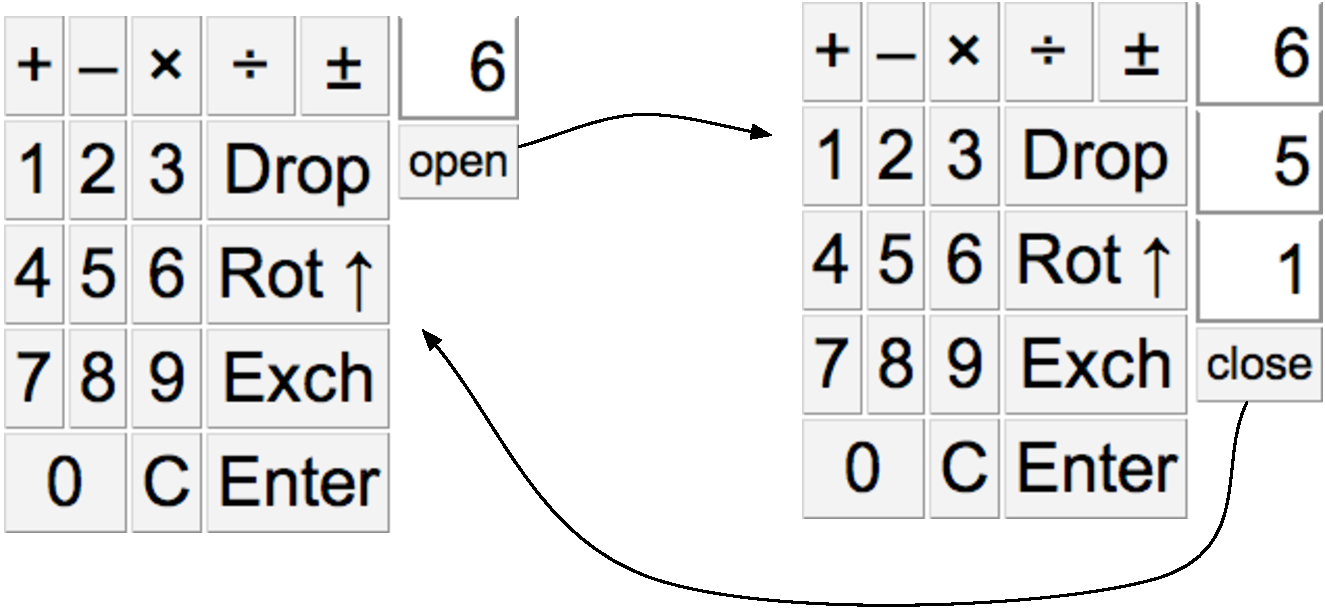
\includegraphics[width=\textwidth]{stackMachine}
\caption{スタックマシンを使ったRPN計算機}
\figlabel{stackMachine}
\end{center}
\end{figure}

スタックマシンの実装を、テストを書きながら始めていきましょう。

\dothis{\ct{contents}というインスタンス変数を持つ\ct{MyStackMachine}というクラスを定義してください。\ct{OrderedCollection}で初期化します。}

\begin{code}{}
MyStackMachine>>>initialize
	super initialize.
	contents := OrderedCollection new.
\end{code}

スタックマシンは\ct{push:}や\ct{pop}をサポートしなければなりません。またスタックの\lct{先頭}を見る機能や、積んだ値に対して加減乗除ができる機能も必要でしょう。

\dothis{スタック操作のテストを書いてから実装してみましょう。以下はテストのサンプルです。}

\needlines{4}
\begin{code}{}
MyStackMachineTest>>>testDiv
	stack
		push: 3;
		push: 4;
		div.
	self assert: stack size = 1.
	self assert: stack top = (4/3).
\end{code}

加減乗除では、事前にスタックに値が二つ積まれているかをチェックするヘルパーメソッドが必要でしょう。条件が整っていない場合はエラーとなるようにします。\footnote{事前条件を指定するには \ct{Object>>>assert:} を使うと良いでしょう。不正な状態でスタックマシンを使おうとしているときには\ct{AssertionFailure}が起こるというわけです。}
これができてしまえば、各メソッドの実装はほぼ一行か二行ですみます。

デバッグしやすくするため、 \ct{MyStackMachine>>>printOn:}も実装しておくと良いでしょう。インスペクタを使って、スタックマシンの状態を観察できるようにします。
(ヒント:  \ct{contents}に表示を委譲してしまうのが楽です)。
\index{Object!printOn:@\ct{printOn:}}

\dothis{ \ct{dup} (先頭の値をコピーしてプッシュする)、 \ct{exch} (スタックの上位二つの値を入れ替える)、 \ct{rotUp} (スタックの内容を上下逆にする\,---\,先頭の要素が最後になる)、を\ct{MyStackMachine} に実装し、スタックマシンを完成させましょう。}

スタックマシンの実装がすんだら、次はいよいよSeaside上に RPN計算機を作っていきます。

クラスを5つ定義することにします:
\begin{itemize}
  \item \ct{MyRPNWidget}\,---\,RPN計算機のコンポーネントで共通に使う振る舞いやCSSを定義するための、抽象クラスです。  \ct{WAComponent}のサブクラスで、以下の4つのクラスのスーパークラスになります。
  
  \item \ct{MyCalculator}\,---\,ルートコンポーネントです。クラスメソッドでアプリケーションの登録を行います。サブコンポーネントを生成し、レンダリングを行わせます。またバックトラック用に状態の登録も行います。
  
  
  \item \ct{MyKeypad}\,---\,計算機のキーパッドを表示します。
  \item \ct{MyDisplay}\,---\,スタックの先頭の値と、詳細なビューに切り替えるためのボタンを表示します。
  \item \ct{MyDisplayStack}\,---\,スタックの詳細なビューと、元のビューに戻るためのボタンを表示します。\lct{MyDisplay}のサブクラスです。

\end{itemize}

\dothis{\ct{MyCalculator}クラスカテゴリに\ct{MyRPNWidget}を定義してみましょう。アプリケーションで共通に使う \ct{style} メソッドを書くようにします。}

アプリケーション用にCSSを定義します。もっと凝ってみてもかまいません。
\begin{code}{}
MyRPNWidget>>>style
	^ 'table.keypad { float: left; }
td.key {
	border: 1px solid grey;
	background: lightgrey;
	padding: 4px;
	text-align: center;
}
table.stack { float: left; }
td.stackcell {
	border: 2px solid white;
	border-left-color: grey;
	border-right-color: grey;
	border-bottom-color: grey;
	padding: 4px;
	text-align: right;
}
td.small { font-size: 8pt; }'
\end{code}

\dothis{ルートコンポーネント\ct{MyCalculator}を定義して、アプリケーションとして登録しましょう(クラスメソッド \ct{canBeRoot} と \ct{initialize} を実装します)。
 \ct{MyCalculator>>>renderContentOn:} では、クラス名の表示などの簡単なレンダリングを書いて、Webブラウザで表示されるかを確認してみましょう。}

\ct{MyCalculator} では、 \ct{MyStackMachine}、\ct{MyKeypad} 、\ct{MyDisplay}のインスタンスを保持することにします。

\dothis{
\lct{MyRPNWidget}のサブクラスとして \ct{MyKeypad}と \ct{MyDisplay}を定義しましょう。コンポーネントはどれもスタックマシンのインスタンスを使うので、インスタンス変数 \ct{stackMachine} と初期化用のメソッド \ct{setMyStackMachine:} を \ct{MyRPNWidget}に用意します。 \ct{MyCalculator}には
 \ct{keypad} と \ct{display} のインスタンス変数を定義し、 \ct{MyCalculator>>>initialize}で初期化することにします。(\lct{super initialize}を送るのを忘れないように!)}

\dothis{
さらにinitializeメソッドでは、stackMachineをkeypadとdisplayに渡すように書いておきます。
レンダリングメソッド \ct{MyCalculator>>>renderContentOn:} の実装は、単にkeypadとdisplayに委譲するだけです。サブコンポーネントを正しく表示するには、\ct{MyCalculator>>>children} を実装して、keypadとdisplayによる配列を返すようにしなければなりません。keypadとdisplayにもレンダリングメソッドを作りますが、中身は空にしておきます。まずはcalculatorがちゃんとサブコンポーネントを表示しているかを確認してみましょう。
}

%\ab{Too long!}

次はdisplayのレンダリングメソッドの中身を書き、スタックの先頭を表示できるようにします。

\dothis{ レンダリングでは、``keypad''というCSSクラス名のテーブルを書き、行には``stackcell''というclassのセルを一つだけ入れることにします。また、スタックが空の場合、先頭に0をpushするようにしておきます。(\ct{MyKeypad>>>ensureMyStackMachineNotEmpty}というメソッドを定義して使うことにします)。さらに``keypad''のクラス名で
セルのデータとしてスタックの値をレンダリングするように書きます。ハロを表示させてみると\figref{firstStackDisplay}のようになるはずです。
}

\begin{figure}[ht]
\begin{center}
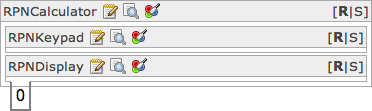
\includegraphics[width=0.8\textwidth]{firstStackDisplay}
\caption{スタックの先頭を表示}
\figlabel{firstStackDisplay}
\end{center}
\end{figure}

今度はスタックとやりとりするためのUIを書いていくことにしましょう。

\dothis{
まず以下のヘルパーメソッドを定義することにします。UIを簡単にかけるようにするためです。
}

\needlines{3}
\begin{code}{}
MyKeypad>>>renderStackButton: text callback: aBlock colSpan: anInteger on: html 
	html tableData
		class: 'key';
		colSpan: anInteger;
		with: 
				[html anchor
					callback: aBlock;
					with: [html html: text]]
\end{code}


\begin{code}{}
MyKeypad>>>renderStackButton: text callback: aBlock on: html 
	self 
		renderStackButton: text
		callback: aBlock
		colSpan: 1
		on: html
\end{code}

これらのメソッドは、キーパッドのボタンを表示しコールバックを定義するために使います。ボタンの中には複数のカラムを占めるものもありますが、基本はカラムを一つ使うことにします。

\dothis{
以下のように二つのヘルパーメソッドを使ってキーパッドのレンダリングを書いてみましょう。
(ヒント: 数値キーと ``Enter'' キーから初めて、計算用のキーは後からつけると楽です)。
}

\needlines{4}
\begin{code}{}
MyKeypad>>>renderContentOn: html 
  self ensureStackMachineNotEmpty.
  html table
    class: 'keypad';
    with: [
      html tableRow: [
          self renderStackButton: '+' callback: [self stackOp: #add] on: html.
          self renderStackButton: '&ndash;' callback: [self stackOp: #min] on: html.
          self renderStackButton: '&times;' callback: [self stackOp: #mul] on: html.
          self renderStackButton: '&divide;' callback: [self stackOp: #div] on: html.
          self renderStackButton: '&plusmn;' callback: [self stackOp: #neg] on: html ].
        html tableRow: [
          self renderStackButton: '1' callback: [self type: '1'] on: html.
          self renderStackButton: '2' callback: [self type: '2'] on: html.
          self renderStackButton: '3' callback: [self type: '3'] on: html.
          self renderStackButton: 'Drop' callback: [self stackOp: #pop]
          	colSpan: 2 on: html ].
"などなど"
        html tableRow: [
          self renderStackButton: '0' callback: [self type: '0'] colSpan: 2 on: html.
          self renderStackButton: 'C' callback: [self stackClearTop] on: html.
          self renderStackButton: 'Enter'
          	callback: [self stackOp: #dup. self setClearMode]
			colSpan: 2 on: html ]]
\end{code}

キーパッドがブラウザできちんと表示されるか確認しましょう。当然ですが、クリックしてみてもまだ計算機としては動作しません。

\dothis{
 \ct{MyKeypad>>>type:} を実装して、タイプした数字がスタックの先頭に反映されるようにしましょう。
入力された値は文字列で得られるので、スタックの値を文字列にして連結し、整数にしてからスタックに戻す必要があります。具体的には以下のようなコードになります。
}

\begin{code}{}
MyKeypad>>>type: aString
	stackMachine push: (stackMachine pop asString, aString) asNumber.
\end{code}
数値キーを打つと、表示が更新されるようになりました。
(\ct{MyStackMachine>>>pop} でポップした値を返すようにきちんと実装していないと、動作しません!)

\dothis{次に\ct{MyKeypad>>>stackOp:}を書くことにしましょう。以下のようにすれば良いでしょう。}

\begin{code}{}
MyKeypad>>>stackOp: op
	[ stackMachine perform: op ] on: AssertionFailure do: [ ].
\end{code}

ポイントはすべての操作が成功するわけではないと言うことです。例えば二つの数値がスタックに積まれていないと、加算できません。当面は単にエラーを無視するように書いておきます。もっと機能を充実させたい場合は、エラーハンドリングのブロックに、ユーザに注意を促すように書いていくことができます。

\dothis{逆ポーランド記法の計算機はこれで一応動くものになりました。
数値キーをいくつか打ってみて、\menu{Enter}キーで値をプッシュしてみましょう。  \menu{+}を押して2つの値が足されることを確認してください。}

数値の入力が予想した動きと若干違うのではないでしょうか。\emph{新たな}数値を入力しているのか、既存の数値を更新しているのかをモードによって区別できないとまずいようです。

\dothis{ \ct{MyKeypad>>>type:}を修正し、モードに応じて動作を変えるようにしてみましょう。 \ct{mode}というインスタンス変数を定義して、3つの値を取るようにします。数値を入力しているときは\lct{\#typing}です。計算ボタンを押した後は、\lct{\#push}モードとなり、入力していた値を強制的にプッシュするようにします。\menu{Enter}を押した後は、\lct{\#clear}となり、次の入力の前にスタックの先頭をクリアします。
 \ct{type:}メソッドを書き直したのが以下のコードです。
}

%モードを設定する部分のコードを載せていないのですごくわかりにくい

\begin{code}{}
MyKeypad>>>type: aString
	self inPushMode ifTrue: [
		stackMachine push: stackMachine top.
		self stackClearTop ].
	self inClearMode ifTrue: [ self stackClearTop ].
	stackMachine push: (stackMachine pop asString, aString) asNumber.
\end{code}
\mb{better with "stackMachine dup" instead of "stackMachine push:
  stackMachine top}"

前よりは入力が便利になりましたが、スタックの先頭の値を見ることができない点がまだ不満です。

\dothis{
\ct{MyDisplay}のサブクラスとして \ct{MyDisplayStack} を定義しましょう。
\ct{MyDisplay}のレンダリングメソッドにボタンの描画を追加して、コールバックで \ct{MyDisplayStack}のインスタンスをcall:するようにします。HTMLのアンカーを使って、以下のように書けるでしょう。
}

\begin{code}{}
html anchor
	callback: [ self call: (MyDisplayStack new setMyStackMachine: stackMachine)];
	with: 'open'
\end{code}
\mb{if the user got a stackmachine ivar, I'm sure he will define
  setStackMachine and not setMyStackMachine}

コールバックが呼ばれると、\ct{MyDisplay} コンポーネントの表示は、一時的に \ct{MyDisplayStack}コンポーネントへと切り替わり、スタックのすべての情報を表示するようになります。\ct{self answer}によって、このコンポーネントが終了して閉じると、制御はもとの\ct{MyDisplay}へと戻ります。

\dothis{
\ct{MyDisplayStack}のレンダリングメソッドを定義して、スタックのすべての内容を表示するようにしましょう。(スタックマシンの\ct{contents}の値を返すアクセッサーを用意するか、 \ct{MyStackMachine>>>do:}を定義して、スタックの値をイテレートできるようにすると良いでしょう)。``close''ボタンもつけることにします。コールバックでは単に\ct{self answer}を実行するだけです。
}

\begin{code}{}
html anchor
	callback: [ self answer];
	with: 'close'
\end{code}

これで\emph{open} と \emph{close}で表示を切り替えられるようになりました。

とはいえ、まだ考慮していなかったこともあります。いくつか操作をしてみた後で、Webブラウザの「戻る」ボタンで戻って、操作をしてみるとどうなるでしょうか。(例えば\menu{open} でスタックの全体を表示させ、\menu{1}、 \menu{Enter}と2回入力し、\menu {+}を押します。この時点でスタックの表示は``2''と``1''となっているはずです。ここで「戻る」ボタンを押してみましょう。スタックは``1''を3つ表示した状態になり、\menu {+}を押すと、``3''が表示されます。つまりバックトラックが動作していないのです。

\dothis{
\ct{MyCalculator>>>states}メソッドを実装し、スタックマシンの\ct{contents}を返すようにしましょう。今度はちゃんとバックトラックが効いています。
}

さて、これで動くアプリケーションができあがりました。乾杯!

%=================================================================
\section{AJAXの利用}

% Original text by Lukas Renggli

\ind{AJAX} (Asynchronous \ind{JavaScript} and \ind{XML}) はクライアント側でJavaScriptを活用することで、、Webアプリケーションをさらにインタラクティブにする技術です。

よく知られたJavaScriptのライブラリとしては \ind{Prototype} (\url{http://www.prototypejs.org}) と \ind{script.aculo.us} (\url{http://script.aculo.us})があります。
Prototypeは、JavaScriptを簡潔に書けるようにするためのフレームワークです。
script.aculo.us は、Prototype上に、アニメーションや、ドラッグ\&ドロップなどをサポートする機能を追加したものです。 Seasideでは ``Scriptaculous''というパッケージを通じて、これらのフレームワークを利用することができます。

Seasideのインストールイメージには、Scriptaculousパッケージが最初から入っています。
最新のバージョンは \url{http://www.squeaksource.com/Seaside}から入手可能です。
\url{http://scriptaculous.seasidehosting.st}でデモを見ることができます。イメージにScriptaculousが入っていれば、\url{http://localhost:8080/javascript/scriptaculous}でも、デモを試せます。

ScriptaculousパッケージではSeasideではおなじみのアプローチが取られています。Smalltalkのオブジェクトを使ってアプリケーションをモデリングすれば、JavaScriptのコードが自動生成されます。

簡単な例として、クライアント側でJavaScriptを使うことで、RPN計算機をより自然なUIに変えていきましょう。
今までは、キーを打つたびにページ全体がリフレッシュされていました。ページはそのままで、クライアントが操作した部分のみが更新されるようにしたいと思います。

\dothis{JavaScriptから表示部分を特定するには、idを振る必要があります。計算機のレンダリングメソッドを以下のように変えましょう。\footnote{チュートリアルの例を自分で実装していない場合は、\url{http://www.squeaksource.com/PharoByExample}から、PBE-SeasideRPNパッケージをロードして、コードを修正していけば良いでしょう。クラスの接頭辞は本書と違い、\ct{My*}ではなく\ct{RPN*}になっています。}}

\begin{code}{}
MyCalculator>>>renderContentOn: html
	html div id: 'keypad'; with: keypad.
	html div id: 'display'; with: display.	
\end{code}

\mb{'keyboard' below should be renamed 'keypad'}
\dothis{キーパッドを押した時に再描画されるようにするには、キーパッド側で表示コンポーネントを知る必要があります。インスタンス変数 \ct{display}を \ct{MyKeypad}に追加します。初期化用のメソッドとして\ct{MyKeypad>>>setDisplay:}を用意し、 \ct{MyCalculator>>initialize}で初期化しましょう。これでボタンにJavaScriptのコードを割り当てることができるようになります。\ct{MyKeypad>>>renderStackButton:callback:colSpan:on:} を以下のように変えましょう。}

\begin{code}{}
MyKeypad>>>renderStackButton: text callback: aBlock colSpan: anInteger on: html 
	html tableData
		class: 'key';
		colSpan: anInteger;
		with: [
			html anchor
				callback: aBlock;
				onClick:				"handle Javascript event"
					(html updater
						id: 'display';
						callback: [ :r |
							aBlock value.
							r render: display ];
						return: false);
				with: [ html html: text ] ]
\end{code}

\mthind{WATagBrush}{onClick:}で \ind{JavaScript}のイベントハンドラを指定しています。
\ct{html updater} によって \ct{SUUpdater}のインスタンスが返ってきます。これはJavaScriptのAjax.Updaterオブジェクト(\url{http://www.prototypejs.org/api/ajax/updater})に該当するSmalltalkのオブジェクトです。
このオブジェクトはAJAXリクエストの送信を行い、返ってきたテキストを使い特定部分の更新を行います。
\ct{id:} によって、updaterにXHTMLのどのDOM要素を更新すべきかを指定しています。この例の場合は'display'のidが振られたdiv要素になります。
\ct{callback:} で、ユーザがボタンを押した時のコールバックをブロックの形で指定します。ブロックの引数\ct{r}は、新たに生成されるレンダラで、これを使ってdisplayのコンポーネントの表示を行います。
(コード上はメソッドの引数となっているhtmlレンダラにもアクセスできますが、コールバックのブロックが評価されるときには無効になっているので注意してください)。コールバック内ではdisplayのコンポーネントをレンダリングする前に、 \ct{aBlock} を評価しています。適切な処理を外から渡して行わせるためです。

\ct{return: false} では、リンクに設定されていた元々のコールバックを呼ばないようにJavaScript側に指定しています。元のコールバックが呼ばれると、ページ全体がリフレッシュされてしまうからです。リンクの \ct{callback:}部分を削除して、コールバックを設定しないようにもできますが、JavaScriptが無効になっていても動作するように、あえてこのようにしています。

\dothis{計算機の数値キーを押してみて、まだページ全体のリフレッシュが行われてしまうことを確認してみてください。(WebページのURLがボタンを押すたびに変わります)。}

クライアント側のJavaScriptの振る舞いを実装したのですが、まだ無効なままです。JavaScriptのイベント処理を有効にしましょう。

\dothis{
計算機の下のツールバーに表示されている \link{Configure} リンクをクリックしてください。
``Add Library:''の部分で \ct{SULibrary}を選び、 \button{Add}ボタンを押して\button{Close}で閉じれば完了です。}

% 要動作確認!

ライブラリを手で追加する代わりに、プログラム的に行うこともできます。Seasideにアプリケーションを登録する際に以下のようにして指定します。

\begin{code}{}
MyCalculator class>>>initialize
	(self registerAsApplication: 'rpn')
		addLibrary: SULibrary
\end{code}

\begin{figure}[ht]
\begin{center}
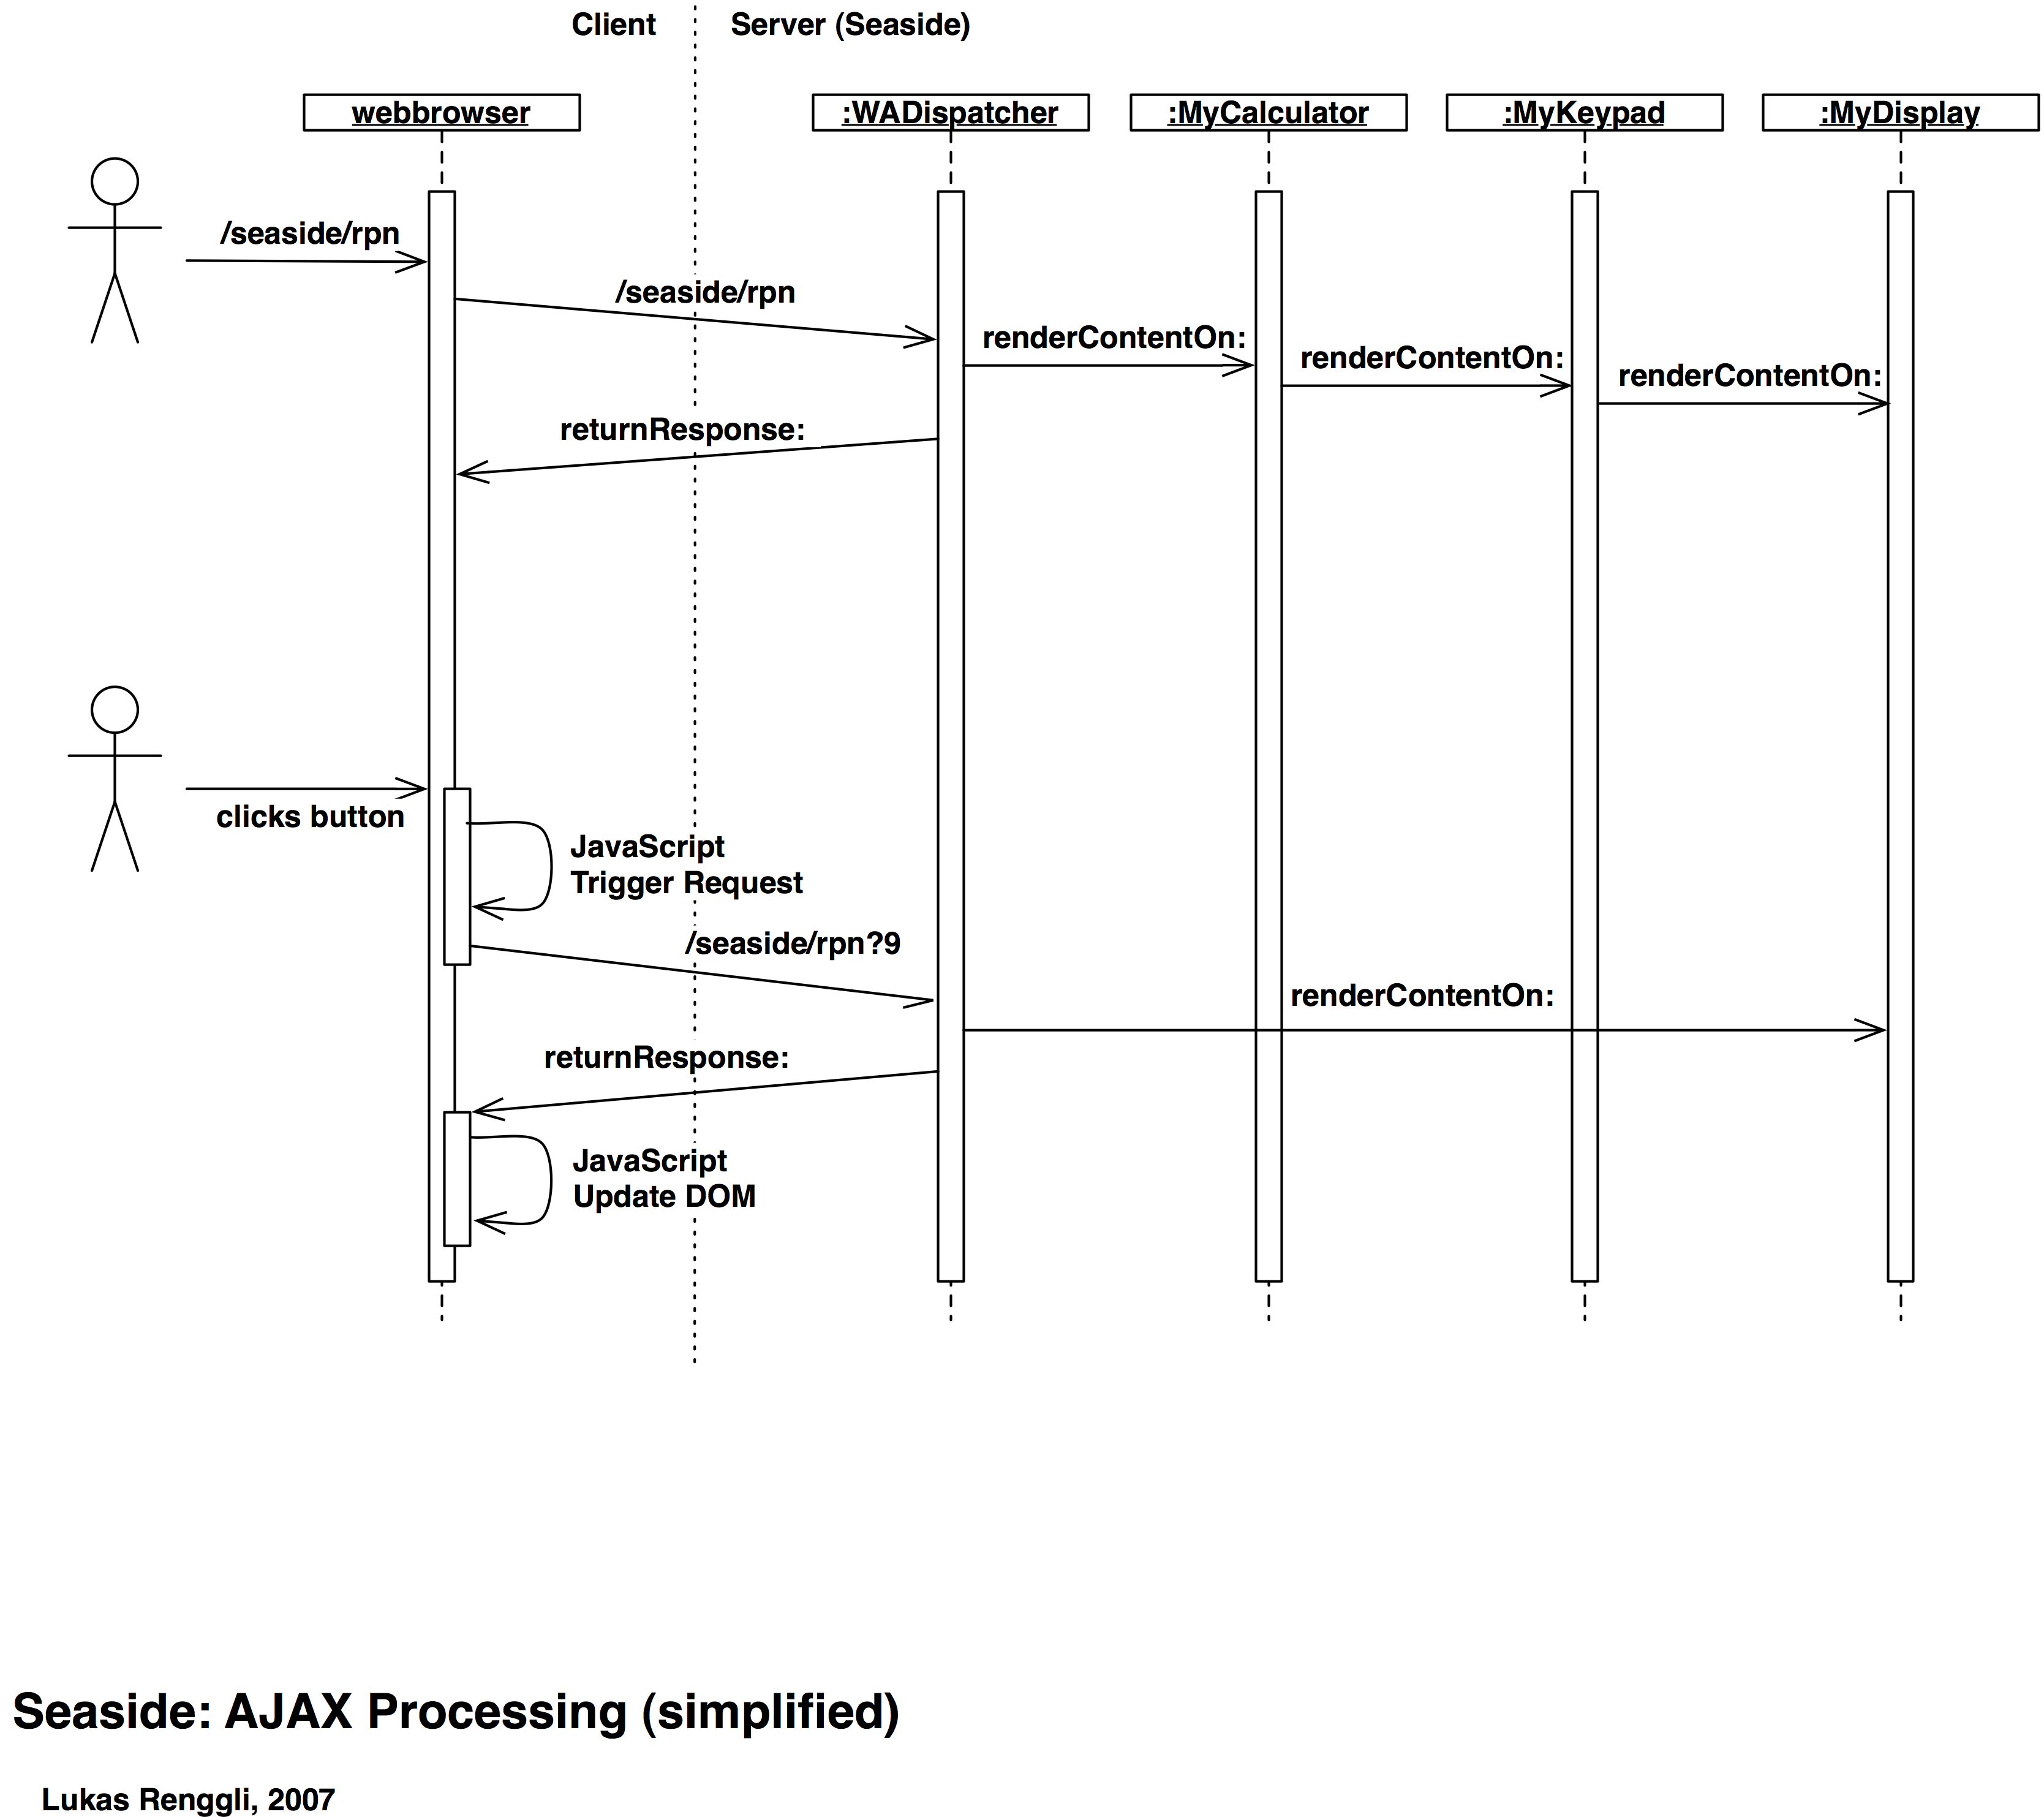
\includegraphics[width=\textwidth]{ajax-processing}
\caption{SeasideでのAJAXの処理(簡略化したもの)}
\figlabel{ajax-processing}
\end{center}
\end{figure}

\dothis{もう一度RPN計算機を試してみましょう。前よりも自然な形で操作できます。キーボタンを押すたびにURLが変わらなくなりました。}

動作は確認できましたが、\emph{仕組みがどうなっているのか}気になるかもしれません。図 \figref{ajax-processing}で、AJAXなしの場合と、有効にした場合とで、RPN計算機のメッセージの流れを示しました。
AJAX の場合は、基本的にレンダリング処理をとばして、displayコンポーネント\emph{のみ}の更新を行います。
JavaScriptはリクエストの送信と、対応するDOM要素の更新の両方を受け持っています。
生成されるJavaScriptのソースを見てみましょう。

\begin{code}{}
new Ajax.Updater(
	'display',
	'http://localhost/seaside/RPN+Calculator',
	{'evalScripts': true,
	  'parameters': ['UNDERSCOREs=zcdqfonqwbeYzkza', 'UNDERSCOREk=jMORHtqr','9'].join('&')});
return false
\end{code}

より高度なサンプルについては \url{http://localhost:8080/javascript/scriptaculous}を見ると良いでしょう。

\paragraph{\emph{Tips}}
サーバ側のデバッグは通常のSmalltalkのデバッガを使うことができます。クライアント側のデバッグはFireFox (\url{http://www.mozilla.com})を入れて、FireBug (\url{http://www.getfirebug.com/}) プラグインを有効にしておくと便利です。

%=================================================================
\section{この章のまとめ}

% item 3 3.0では当てはまらず
% item 5 3.0では当てはまらず
% item 7 3.0ではObsolete
% item 19 3.0では当てはまらず

\begin{itemize}
  \item Seasideを始めるには``Seaside One-Click Experience''イメージを \url{http://seaside.st}からダウンロードするのがもっとも簡単です。
  \item \ct{WAKom startOn: 8080} でサーバを開始、 \ct{WAKom stop}で終了です。
  \item 管理用のIDとパスワードは\ct{WADispatcherEditor initialize}で初期化できます。
  \item \menu{Toggle Halos} をクリックすると、コンポーネントのソースコードやオブジェクトの状態、CSSやXHTMLを見ることができます。
  \item \ct{WAGlobalConfiguration setDeploymentMode} で開発用のツールバーを隠せます。
  \item Seasideのアプリケーションはコンポーネントからできています。コンポーネントとは\ct{WAComponent}を継承したクラスのインスタンスのことです。
  \item SeasideのWeb管理ツールからアプリケーションとして登録できるコンポーネントを、ルートコンポーネントと呼びます。クラスメソッドの \ct{canBeRoot} を実装してtrueを返すようにします。initializeのクラスメソッドで、 \ct{self registerAsApplication:} を自身に送ることで、登録することもできます。引数は \emph{アプリケーションのパス}になります。 \ct{description} をオーバーライドするとWeb上のコンフィギュレーションエディタにアプリケーションの説明を表示させることも可能です。
  \item 状態をバックトラックできるようにするには、コンポーネントで \ct{states} メソッドを定義して、復元したいオブジェクトの配列を返すように実装する必要があります。ユーザが「戻る」ボタンを押しても状態が正常に保たれます。
  \item コンポーネントは\ct{renderContentOn:}を実装することで、自身をWebページ内に表示させることができます。引数としてXHTMLレンダリング用の\emph{キャンバス}が渡ってきます(通常は\ct{html}という名前になっています)。
  \item コンポーネントは、自身が含むサブコンポーネントを \ct{self render:} \emph{subcomponent}で表示させることができます。
  \item XHTMLは \emph{brushes}にメッセージを送ることで生成されます。キャンバスに対して、 \ct{paragraph} や \ct{div}などのメッセージを送ると、XHTML要素に対応したブラシが返ってきます。
  \item ブラシに\ct{with:}を含んだメッセージを連続して送るときは、必ず \ct{with:}が最後になるようにします。\ct{with:}によってXHTML生成が終わり、その結果がレンダリングされるからです。
  \item 状態を操作するアクションはコールバックの中で書くようにします。レンダリングメソッド内でコンポーネントの状態を変えてはいけません。
  \item ブラシに\ct{on:} \emph{instance variable} \ct{of:} \emph{object}を送ることで、フォームの要素やリンクに対し、インスタンス変数の値を簡単に結びつけることができます。
  \item スタイルシートの文字列を返す、\ct{style}メソッドを実装すると、コンポーネントが使うCSSを、クラス階層中に定義できます。(通常デプロイ時には、外部のCSSを固定のURLで参照させるようにします)。
  \item 制御フローは、\ct{x call: y}のように書くことで表せます。この場合、\ct{x}のコンポーネントは \ct{y}のコンポーネントへと置き換えられます。 \ct{y} は \ct{answer:} で制御をxに戻すことができます。\ct{call:}のレシーバはたいていは \ct{self}ですが、それ以外のコンポーネントであってもかまいません。
  \item 制御フローは \emph{タスク}として表すこともできます。タスクは\ct{WATask}のサブクラスとして定義します。 \ct{go}メソッドの中に、ワークフローを、連続した\ct{call:}のメッセージ送信として書いていきます。
  \item ユーザと簡単なやりとりを行うため、\ct{WAComponents}の便利メソッドとして、\ct{request:}、 \ct{inform:}、 \ct{confirm:}、\ct{chooseFrom:caption:} が用意されています。
  \item ユーザが「戻る」ボタンを押して以前の状態にアプリケーションを戻してしまうのを防ぐには、\ct{isolate:}を使います。ブロックでワークフローを分割することで、ブロックを越えて過去の状態に戻ることができなくなります。
\end{itemize}
%-----------------------------------------------------------------

%=================================================================
\ifx\wholebook\relax\else 
   \bibliographystyle{jurabib}
   \nobibliography{scg}
   \end{document}
\fi
%=================================================================
